\subsection{Experiments Configuration Details}

The baseline experiment configuration parameters are presented in Table~\ref{tab:baseline_config}. The simulation parameters were selected based on the observation of simulations. For instance, in most simulations, no more than one type of agent survives after \~80 steps; thus, we select the maximum simulation step as 80. The initial agent amount and moral types are designed considering the cost of the LLM token and the balance between these moral types. For the agent parameters, most of them were selected according to the common sense of the relative relationships of different parameters, such as age vs. minimum age for reproduction, and HP vs. offspring initial HP, etc. For the resource parameters, they are mainly selected to match some agent parameters rationally, such as agent physical ability vs. prey HP and physical ability. The number of resources, HP per resource, and respawn frequency are determined based on different levels of resource abundance for 8 agents to survive and reproduce.

The framework can run on macOS and Linux systems. All experiments were conducted on a computing infrastructure equipped with an NVIDIA GeForce RTX 4090 GPU and a 13th Gen Intel(R) Core(TM) i9-13900KF. The system has 128 GB of RAM and operates on Ubuntu 22.04.5 LTS. All the used software libraries and frameworks are included in the configuration file of our code base. We also used macOS (M2 chip) to develop the framework and run experiments.

To investigate the factors that affect the evolution and agent interaction mechanisms, we conducted several experiments with various settings and evaluation metrics, including evolutionary games with different settings, validation of agent behavior-morality alignment, and mini-games of team forming and HP sharing. 

\begin{table*}[htbp]
\centering
\small
\begin{tabular}{lp{1.2cm}p{6.5cm}}
\hline
\textbf{Parameter} & \textbf{Value} & \textbf{Description} \\
\hline
\multicolumn{3}{l}{\textbf{Simulation Parameters}} \\
\hline
Max time steps & 80 & Total number of time steps the simulation will run. \\
Social interaction steps & 2 & Number of steps designated for social rounds. \\
Other agent moral type visibility & Visible & Whether agents can observe others' moral types. \\

\hline
\multicolumn{3}{l}{\textbf{Agent Parameters}} \\
\hline
Initial Agent Count & 8 & Total number of agents at initialization. \\
Agent type distribution &  & Proportions of each behavioral archetype. \\
-- Universal group morality & 25\% &  \\
-- Reciprocal group morality & 25\% &  \\
-- Kin-focused morality & 25\% &  \\
-- Reproductive selfishness & 25\% &  \\
Steps of recent activities perceivable & 15 & Number of previous steps an agent can perceive. \\
Initial HP & 20 & Initial health points of agents. \\
Max HP & 40 & Maximum health points of agents. \\
Initial age & 10 & Initial age of agents. \\
Max age & 20 & Maximum age of agents. \\
Min HP for reproduction & 12 & Minimum HP threshold for reproduction. \\
HP cost for reproduction & 10 & HP cost for reproduction action. \\
Minimum age for reproduction & 4 & Minimum age threshold for reproduction. \\
Offspring initial HP & 3 & Initial HP of newly created offspring. \\
Physical ability (mean, std) & 6, 0 & Mean and standard deviation of agent ability. \\
Physical scaling (slope, intercept) & 5, 0.1 & Slope and intercept for ability-based interactions. \\
\hline
\multicolumn{3}{l}{\textbf{Resource Parameters}} \\
\hline
Plant: Initial quantity & 4 & Starting number of edible units per plant. \\
Plant: Capacity & 3 & Maximum capacity for plant nodes. \\
Plant: Respawn delay & 10 steps & Turns required before depleted plants respawn. \\
Plant: Nutrition & 3 & HP restored per unit consumed. \\
Prey: Initial quantity & 4 & Initial number of prey in the environment. \\
Prey: HP (mean, std) & 5, 1 & Mean and standard deviation of prey health points. \\
Prey: Physical ability & 4 & Physical ability value of prey. \\
Prey: Respawn rate & 0.1 & Probability of new prey spawning per step. \\
Prey: Max quantity & 6 & Maximum number of prey allowed in environment. \\
Prey: Difficulty & 2 & Abstract scaling factor for prey behavior/resistance. \\
Resource abundance & 2 & Global multiplier for resource density. \\
\hline
\multicolumn{3}{l}{\textbf{LLM Parameters}} \\
\hline
Provider & OpenAI & LLM provider name. \\
Model & GPT-4.1-mini-2025-04-14 & Identifier for the chat model used. \\
Max retries & 10 & Number of retries for failed LLM actions. \\
Reflection round & Enabled & Whether two-stage prompting is used. \\
\hline
\end{tabular}
\caption{This table shows the configuration parameters, their descriptions, and the values used for baseline experiments. Other experiments change only their appropriate parameters: for resource scarcity, we change the resource abundance to 1x; for high communication cost, we change the social interaction steps to 1; for moral type observability, we change the visibility of other agents' moral types to be invisible.}
\label{tab:baseline_config}
\end{table*}


\subsection{Additional Results of Evolutionary Games}
Based on the main baseline experiment mentioned in the main paper, other experiments change only their appropriate parameters: for resource scarcity, we change the resource abundance to 1x; for high communication cost, we change the social interaction steps to 1; for moral type observability, we change the visibility of other agents' moral types to be invisible. And we also tested scenarios where only one type of morality exists in the simulation.
In this section, we present the simulation results from several perspectives.

\subsubsection{Population and selected agents' HP curve}
Besides the main baseline experiments, we conducted simulations with various environment settings.
This section visualizes the dynamics of agent populations and their proportion over time, as well as selected agents' health points (HP) across each simulation setting. 
For each simulation scenario, the figures include:
1) Population Trends: Line plots showing the ratio and count of agent types (e.g., survival, extinction) over time. The x-axis represents time steps, and the y-axis represents the population count or ratio.
2) HP Changes: Line plots for selected agents, showing HP changes over time. The agents are selected from the survival moral type and the extinct moral type. Legends indicate actions (e.g., hunting, resting) that cause HP gain or loss.

% \textbf{Baseline experiment}

\begin{figure}[H]
    \centering
    \begin{subfigure}[t]{0.5\textwidth}
        \centering
        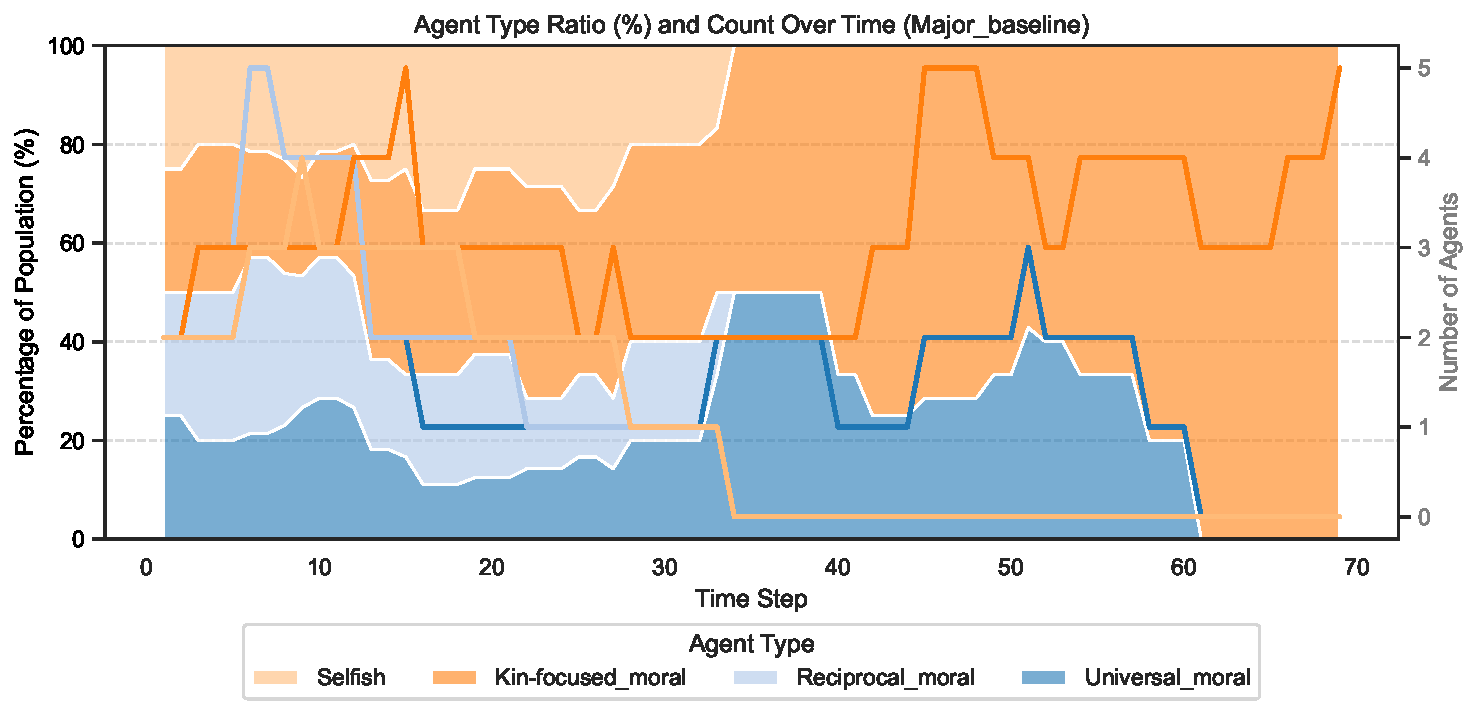
\includegraphics[width=\linewidth]{appendix_figures/populations/population_Major_baseline.pdf}
        \caption{Agent type ratio and count over time}
    \end{subfigure}
    \hfill
    
    \begin{subfigure}[t]{0.48\textwidth}
        \centering
        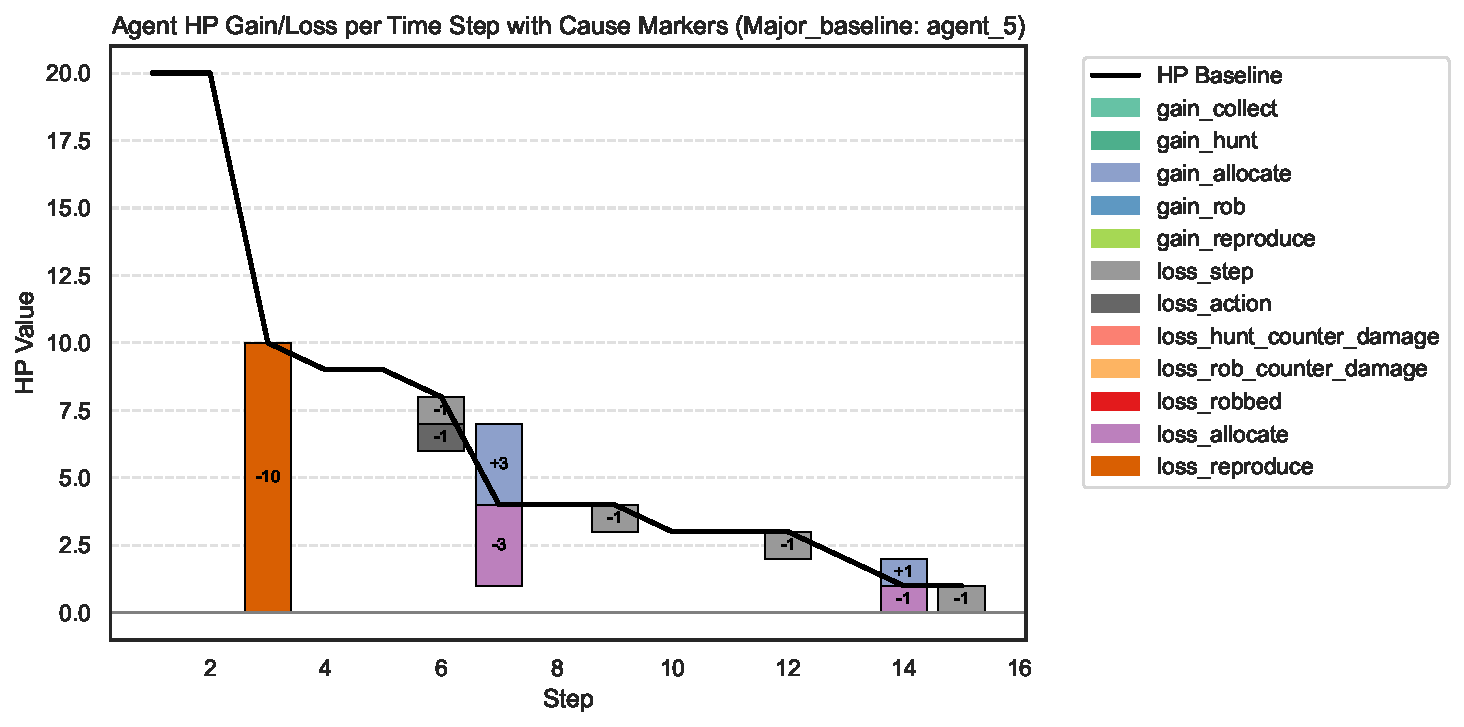
\includegraphics[width=\linewidth]{appendix_figures/HP/hp_change_Major_baseline_agent_5.pdf}
        \caption{HP and causes of an agent from a survival type}
    \end{subfigure}
    \hfill
    \begin{subfigure}[t]{0.48\textwidth}
        \centering
        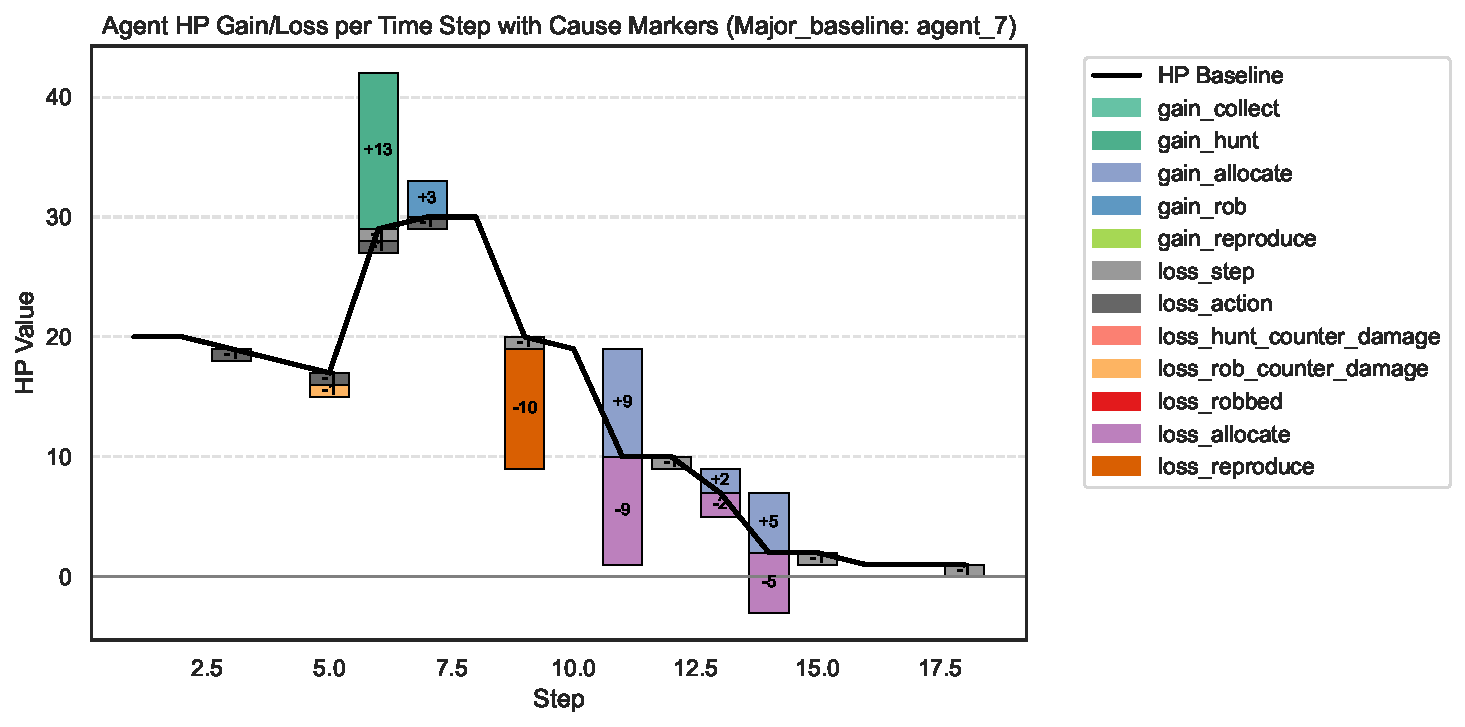
\includegraphics[width=\linewidth]{appendix_figures/HP/hp_change_Major_baseline_agent_7.pdf}
        \caption{HP and causes of an agent from an extinct type}
    \end{subfigure}
    \caption{Agent type ratio and count, and two example agent HP over time (Case: major baseline)}
    \label{fig:main_pop}
\end{figure}


\textbf{Resource Scarcity}
We manipulate resource parameters (quantity, spawning rates, nutritional yield, and acquisition difficulty of plants and prey) through an integrated abundance variable that proportionally adjusts these parameters. For this experiment, we simulate an abundant and a scarce setting of the resources to see how that triggers the evolution of different moral types. 

When the resource is abundant, as shown in Figure~\ref{fig:abundant_pop}, the evolution trends of all types of agents are fairly similar, especially in the early period. This reflects that abundant resource brings enough support for each agent to survive. However, in the end, the selfish and reciprocal agents dominate the world, indicating that their focus on self-interest helps them keep occupying resources.

\begin{figure}[H]
    \centering
    \begin{subfigure}[t]{0.5\textwidth}
        \centering
        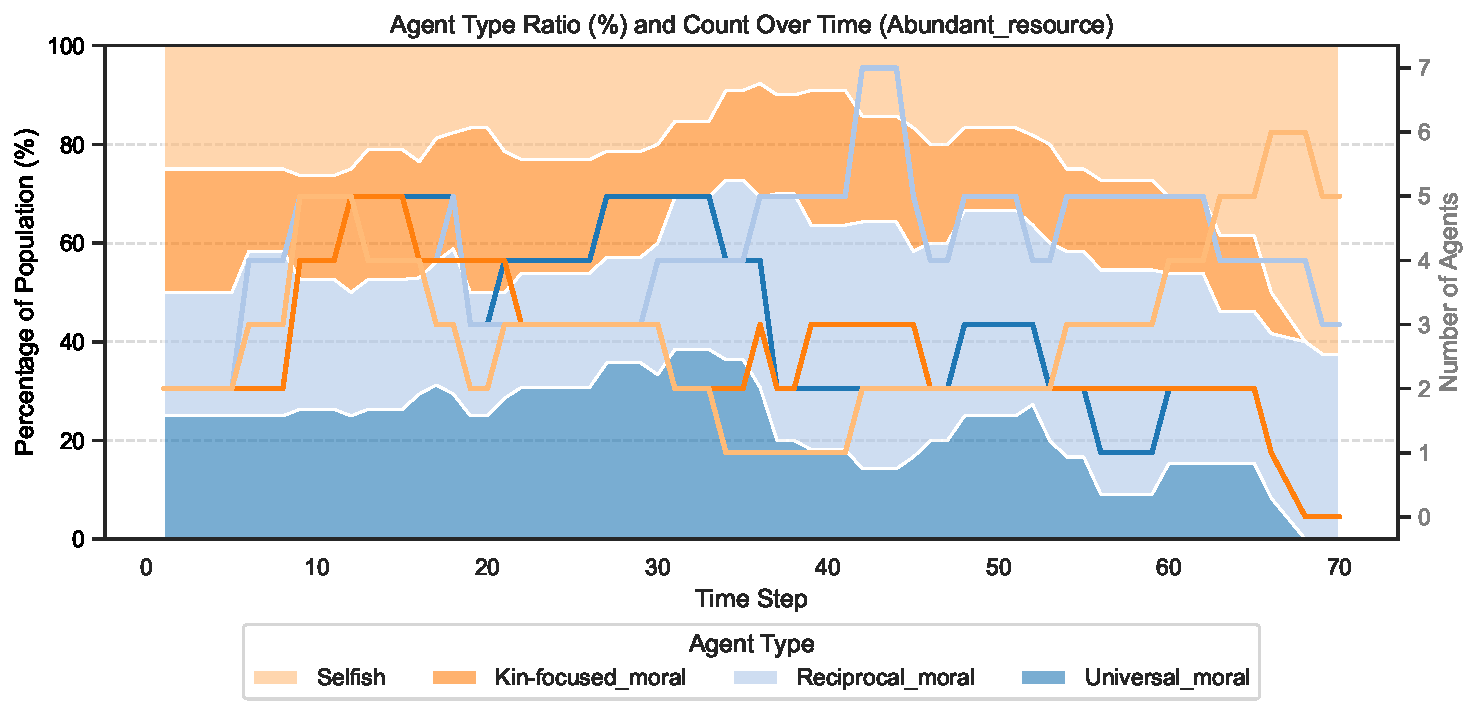
\includegraphics[width=\linewidth]{appendix_figures/populations/population_Abundant_resource.pdf}
        \caption{Agent type ratio and count over time}
    \end{subfigure}
    \hfill
    
    \begin{subfigure}[t]{0.48\textwidth}
        \centering
        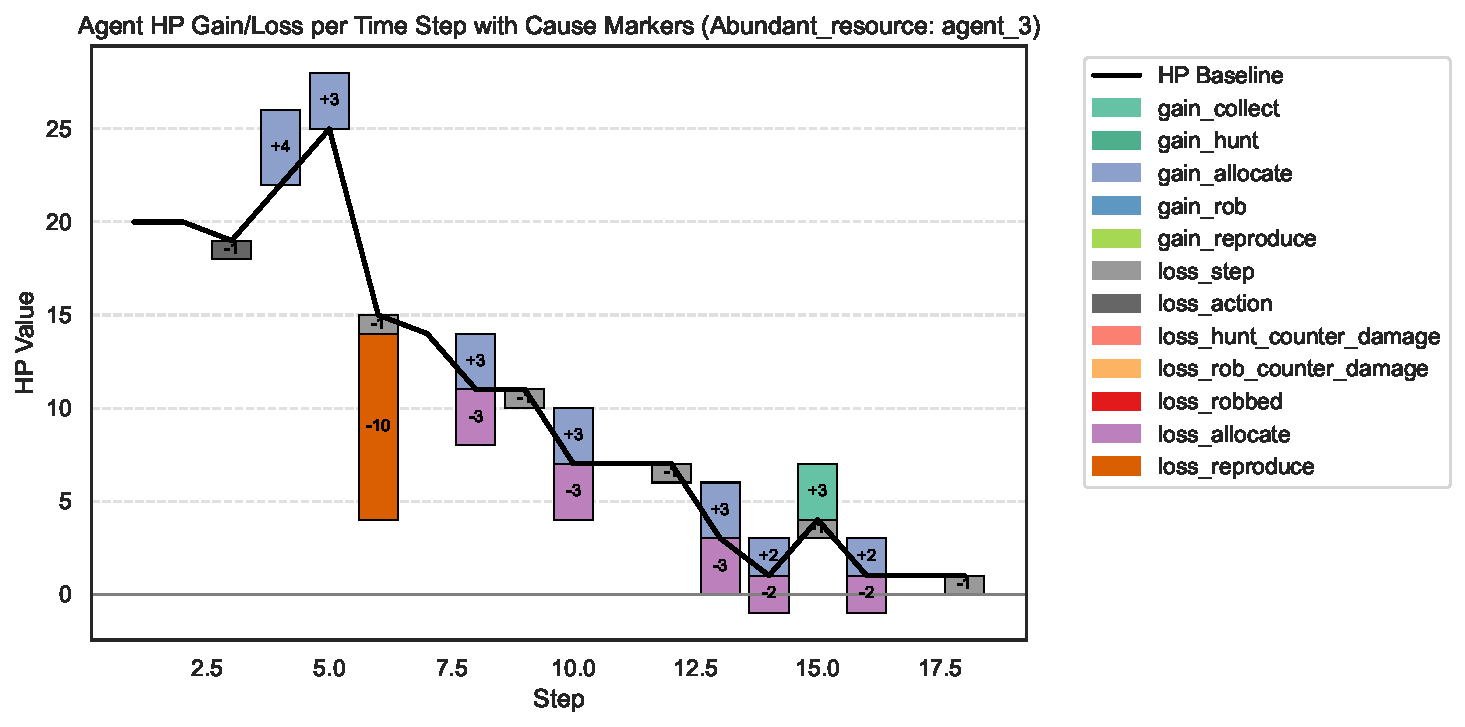
\includegraphics[width=\linewidth]{appendix_figures/HP/hp_change_Abundant_resource_agent_3.pdf}
        \caption{HP and causes of an agent from a survival type}
    \end{subfigure}
    \hfill
    \begin{subfigure}[t]{0.48\textwidth}
        \centering
        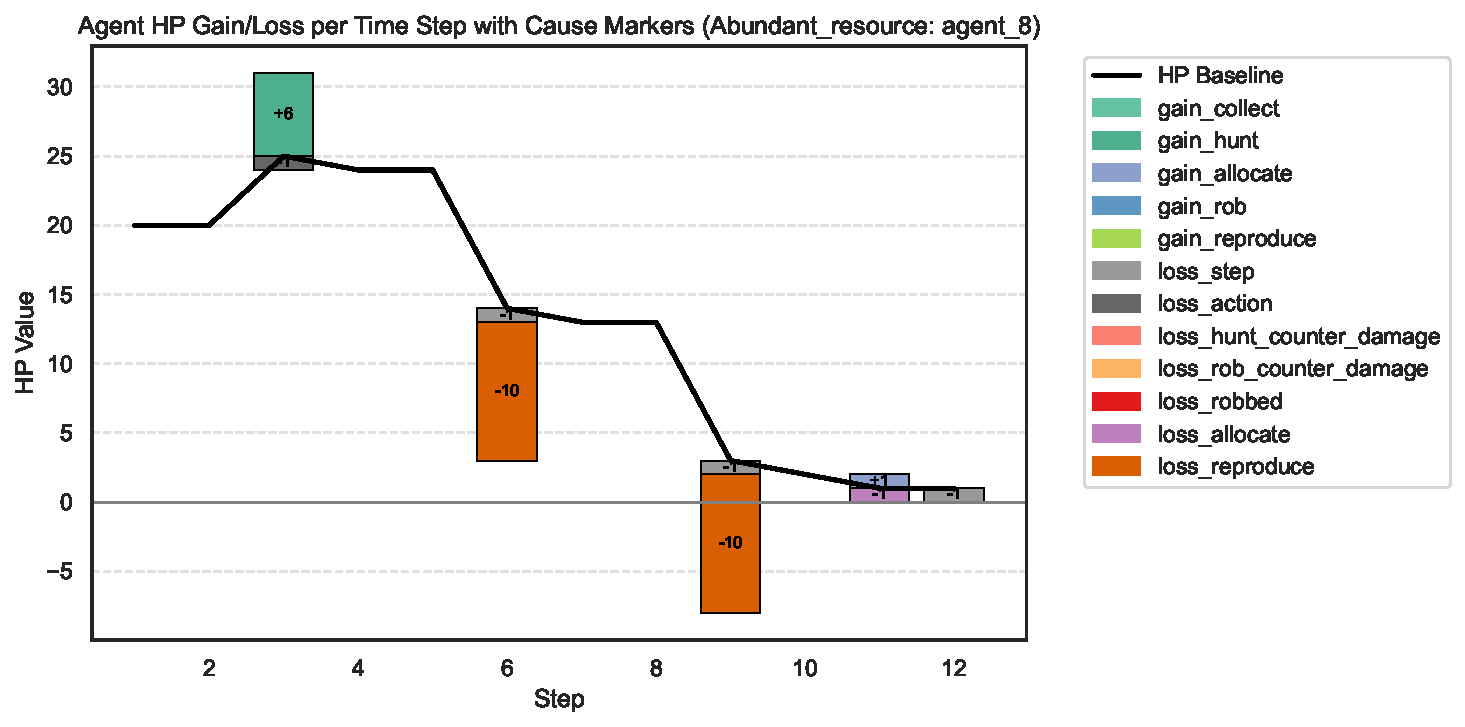
\includegraphics[width=\linewidth]{appendix_figures/HP/hp_change_Abundant_resource_agent_8.pdf}
        \caption{HP and causes of an agent from an extinct type}
    \end{subfigure}
    \caption{Agent type ratio and count, and two example agent HP over time (Case: abundant resource)}
    \label{fig:abundant_pop}
\end{figure}

When the resource is scarce, as shown in Figure~\ref{fig:scarce_pop}, the experiment sees a draw among kin-focused, reciprocal, and selfish, with selfish eventually winning. But looking into the close dynamics, it actually shows that more moral agents are actually more competitive in the process, but the selfish agents moved fast and took a lot of resources at the beginning, getting a head lead that eventually leads to their survival. These experiments show the complexity in the competition - many factors are involved, and unnoticed ones can be fatal.

\begin{figure}[H]
    \centering
    \begin{subfigure}[t]{0.5\textwidth}
        \centering
        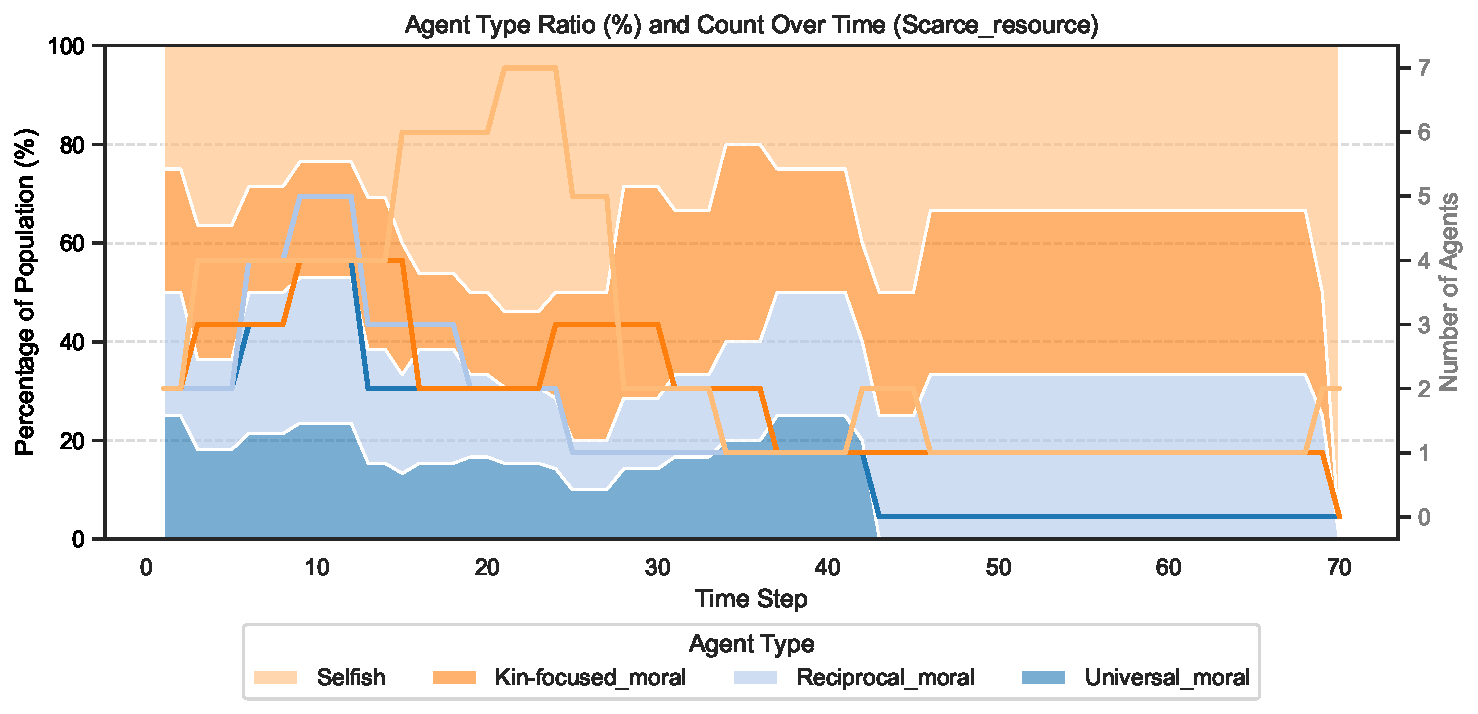
\includegraphics[width=\linewidth]{appendix_figures/populations/population_Scarce_resource.pdf}
        \caption{Agent type ratio and count over time}
    \end{subfigure}
    \hfill
    \begin{subfigure}[t]{0.48\textwidth}
        \centering
        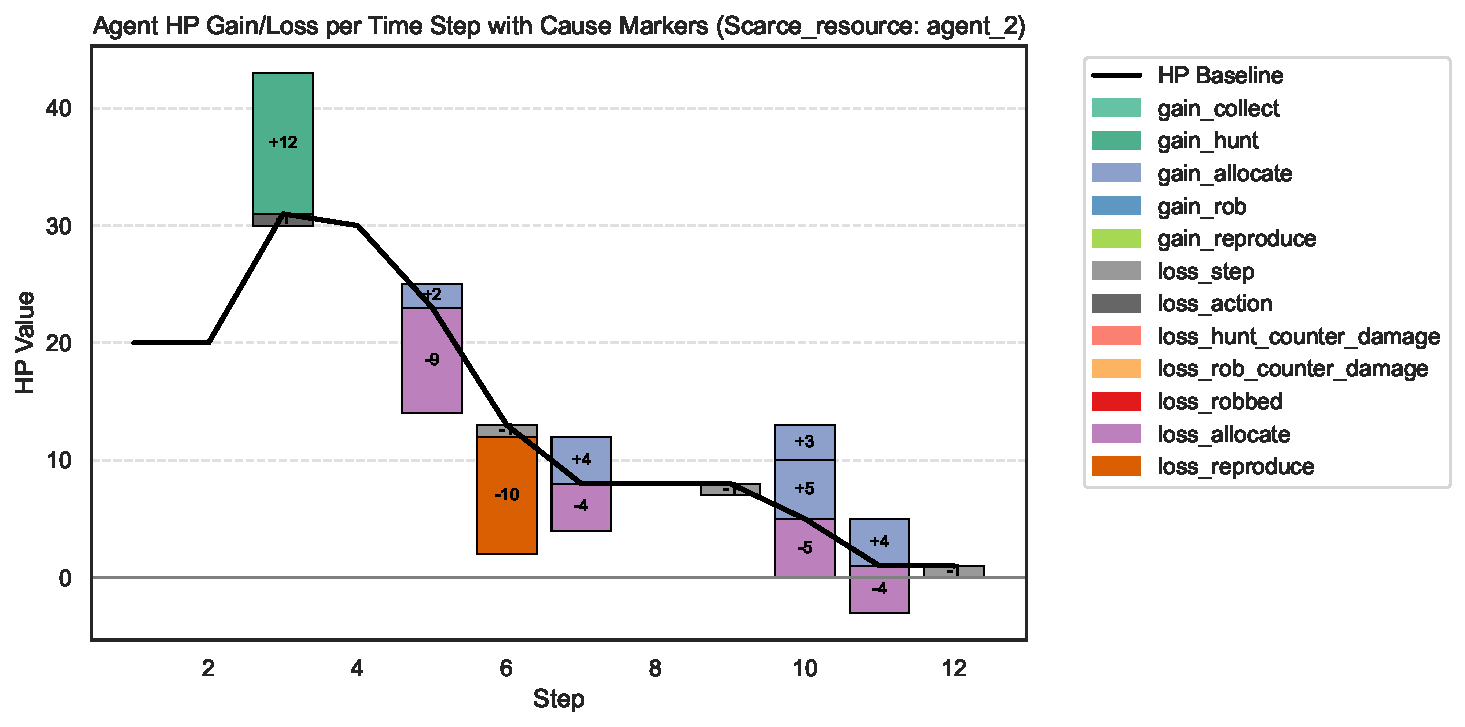
\includegraphics[width=\linewidth]{appendix_figures/HP/hp_change_Scarce_resource_agent_2.pdf}
        \caption{HP and causes of an agent from a survival type}
    \end{subfigure}
    \hfill
    \begin{subfigure}[t]{0.48\textwidth}
        \centering
        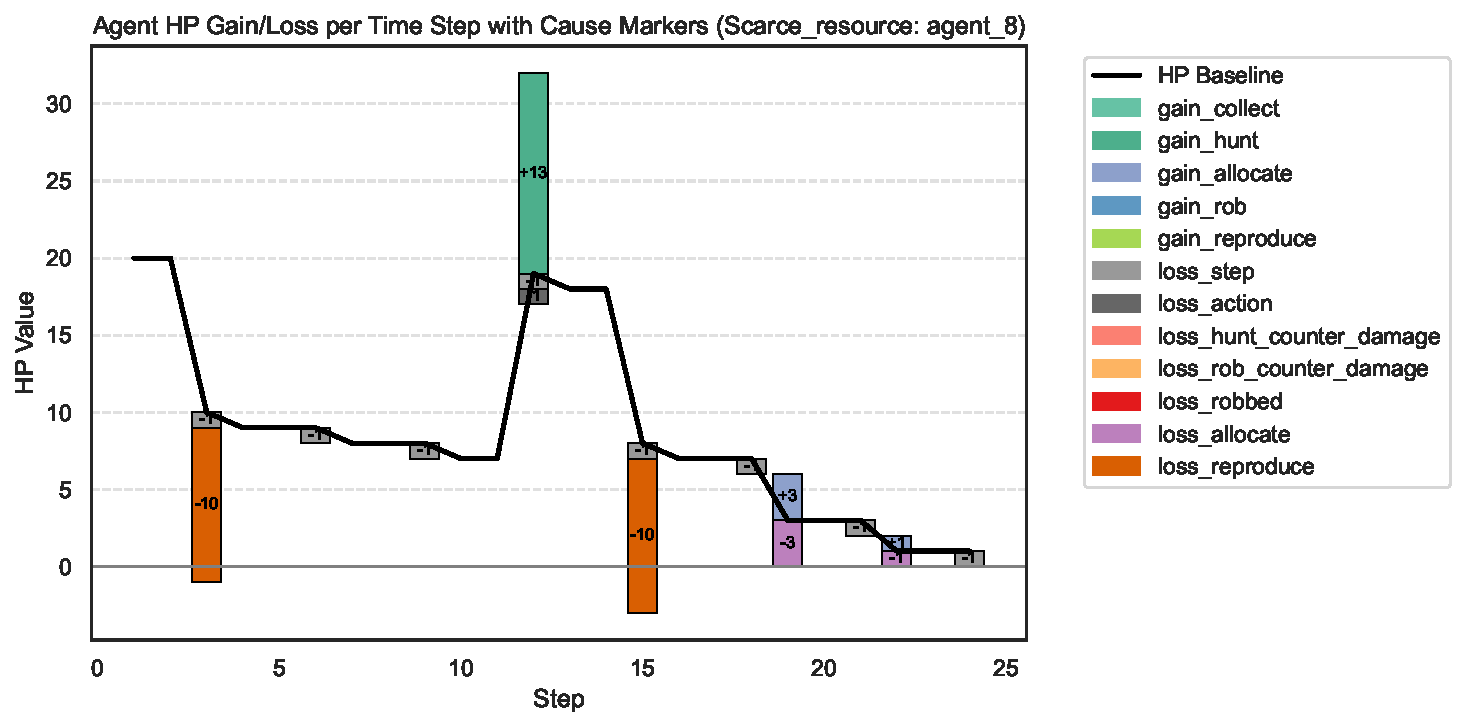
\includegraphics[width=\linewidth]{appendix_figures/HP/hp_change_Scarce_resource_agent_8.pdf}
        \caption{HP and causes of an agent from an extinct type}
    \end{subfigure}
    \caption{Agent type ratio and count, and two example agent HP over time (Case: scarce resource)}
    \label{fig:scarce_pop}
\end{figure}


\textbf{Moral Type Observability}
The ability to accurately identify others' moral dispositions represents a critical cognitive capability affecting cooperation dynamics. When moral types are directly observable, agents can avoid misattributing intentions and form more stable cooperative relationships. We investigate how this observability capability influences which moral types achieve evolutionary dominance under otherwise identical conditions. As shown in Figure \ref{fig:invisible_pop} (b), the kin and universal moral agents stay in the end while others die out early. Reciprocal moral agents did not survive because he was mistaken as selfish agents due to misjudgment. This shows that the ability to let others know your true moral type is critical for the survival of moral agents.

\begin{figure}[H]
    \centering
    \begin{subfigure}[t]{0.5\textwidth}
        \centering
        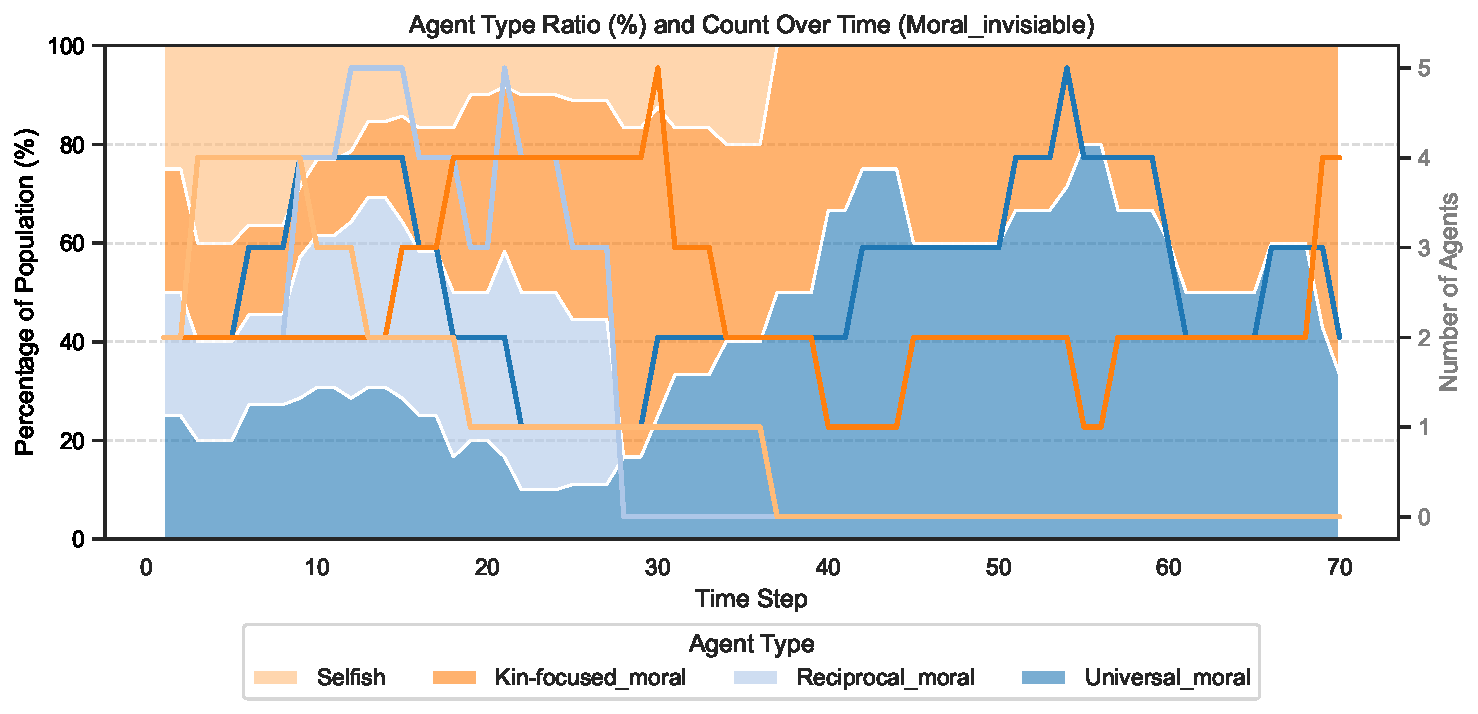
\includegraphics[width=\linewidth]{appendix_figures/populations/population_Moral_invisiable.pdf}
        \caption{Agent type ratio and count over time}
    \end{subfigure}
    \hfill
    
    \begin{subfigure}[t]{0.48\textwidth}
        \centering
        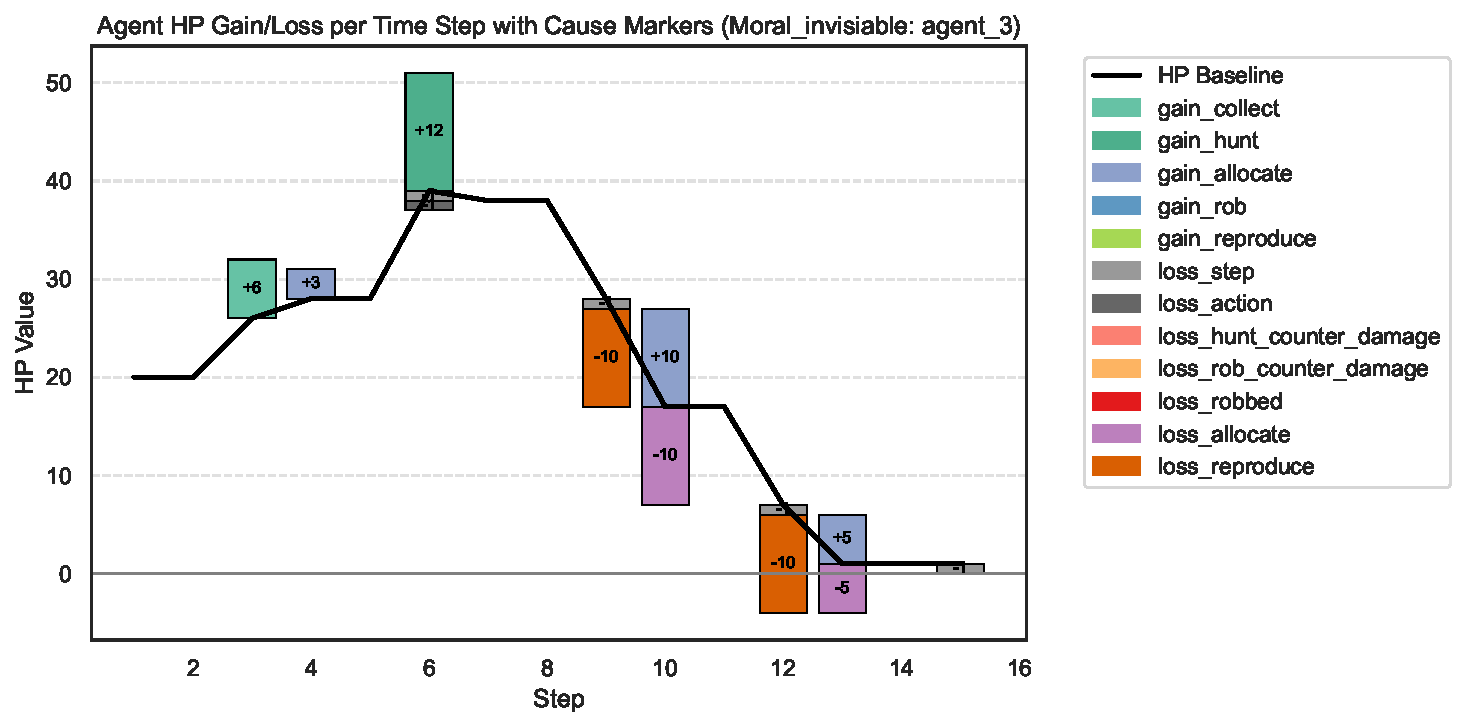
\includegraphics[width=\linewidth]{appendix_figures/HP/hp_change_Moral_invisiable_agent_3.pdf}
        \caption{HP and causes of an agent from a survival type}
    \end{subfigure}
    \hfill
    \begin{subfigure}[t]{0.48\textwidth}
        \centering
        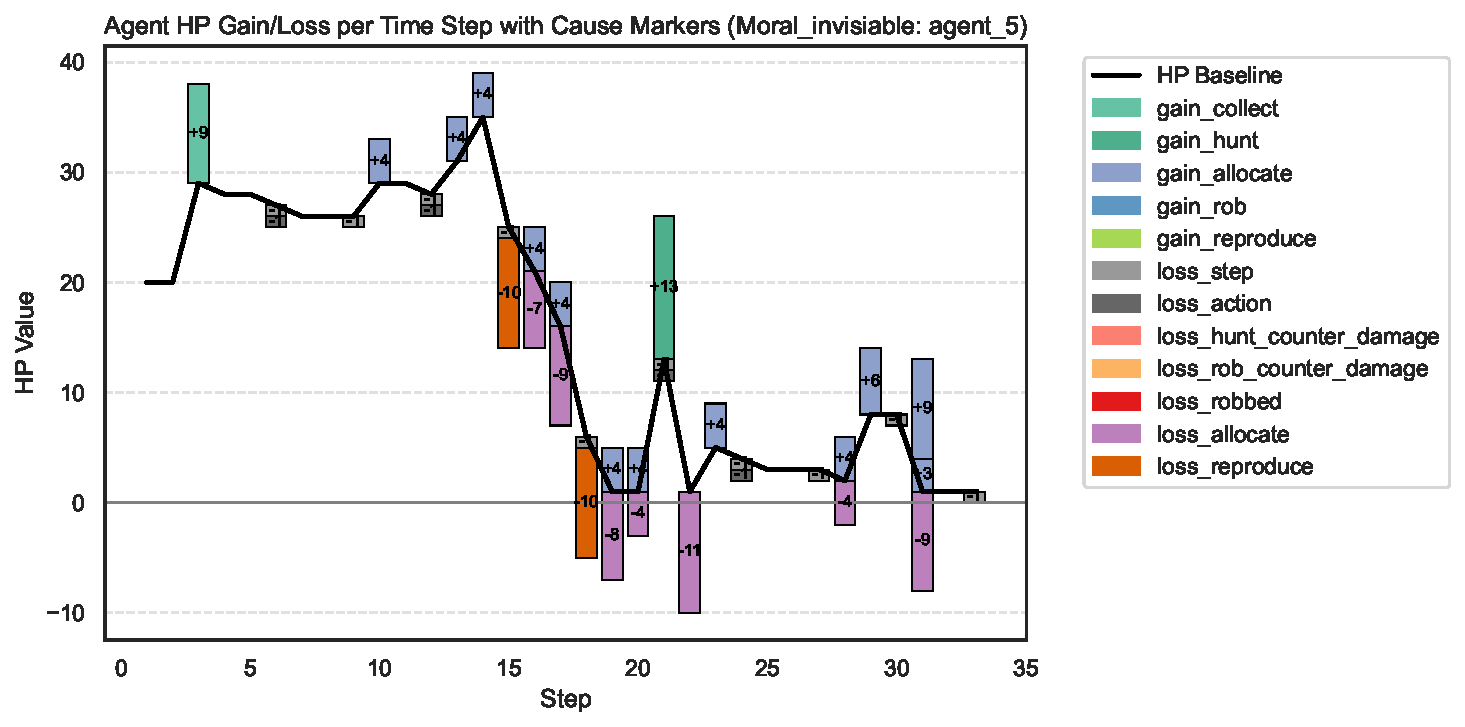
\includegraphics[width=\linewidth]{appendix_figures/HP/hp_change_Moral_invisiable_agent_5.pdf}
        \caption{HP and causes of an agent from an extinct type}
    \end{subfigure}
    \caption{Agent type ratio and count, and two example agent HP over time (Case: moral invisible)}
    \label{fig:invisible_pop}
\end{figure}

\textbf{Social Interaction Cost}
To model the differential temporal scales of social versus productive activities, we implement adjustable time costs for social interactions. Our framework allows varying numbers of social interaction rounds (communication, fighting) before agents can undertake resource acquisition or reproduction. This mechanism enables flexible control over the relative investment required for social engagement versus production. 
This experiment investigates a high social interaction cost by allowing only 1 social interaction round before production, making the communication extremely hard. As we can see in Figure \ref{fig:cost_pop} (c), the selfish agents clearly dominate the population. The reason is that the high communication cost makes the collaboration extremely hard, so moral agents spend more time getting together to take productive actions. Meanwhile, selfish agents just go take actions directly, obtaining an advantage.

\begin{figure}[H]
    \centering
    \begin{subfigure}[t]{0.5\textwidth}
        \centering
        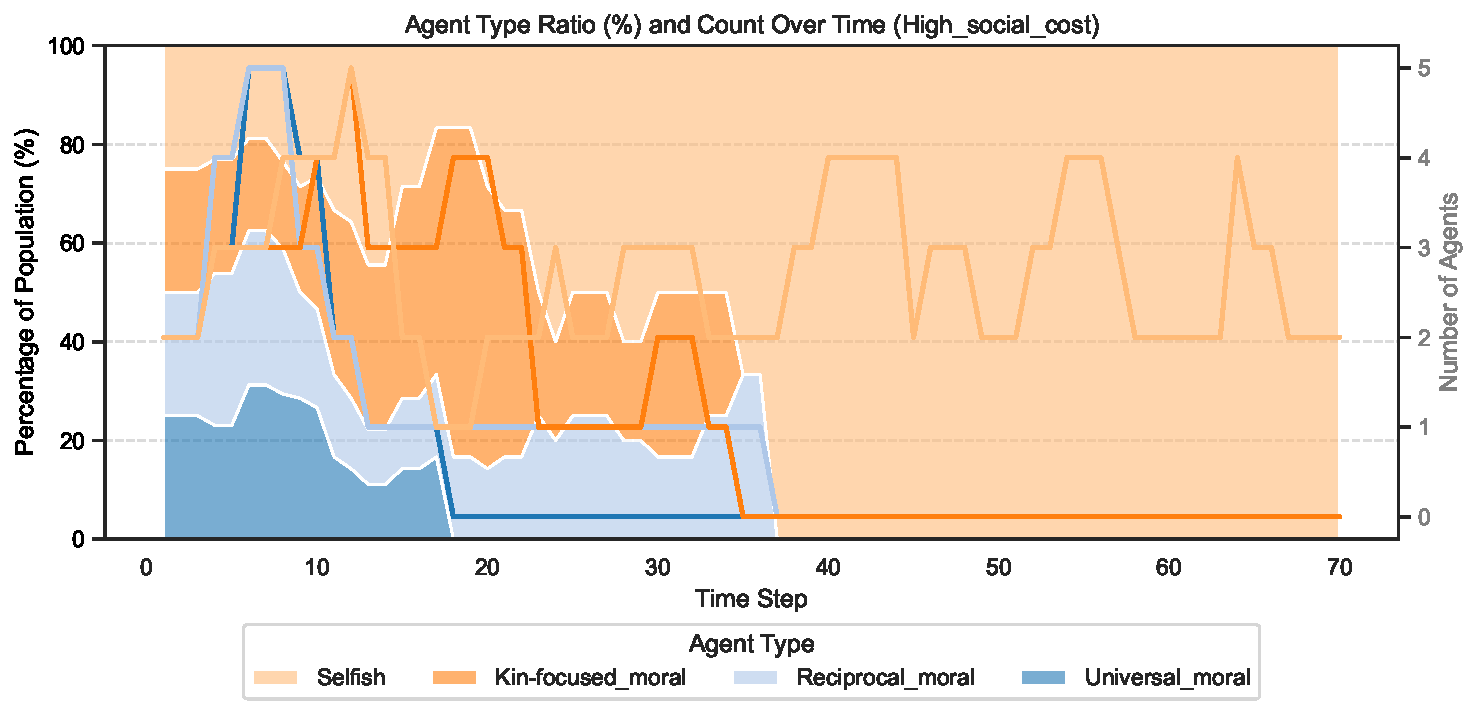
\includegraphics[width=\linewidth]{appendix_figures/populations/population_High_social_cost.pdf}
        \caption{Agent type ratio and count over time}
    \end{subfigure}
    \hfill
    
    \begin{subfigure}[t]{0.48\textwidth}
        \centering
        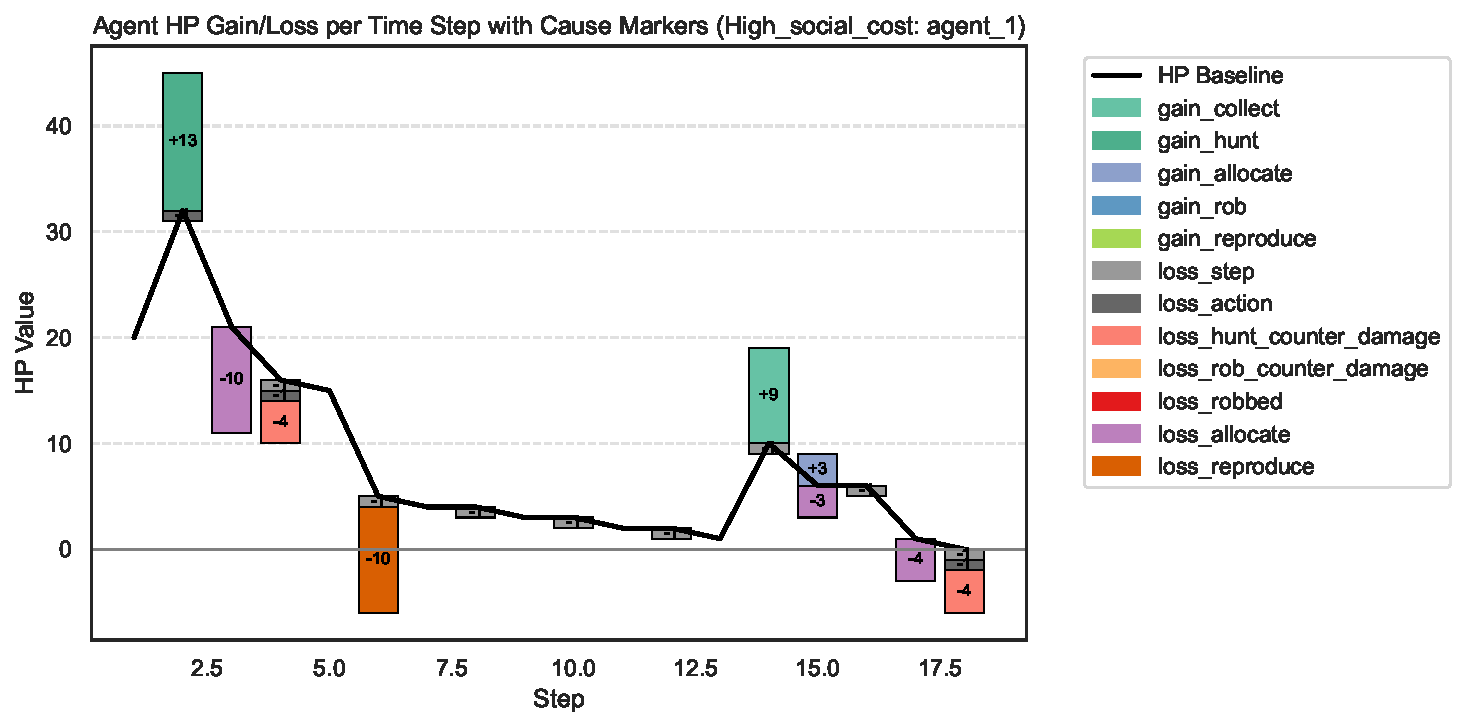
\includegraphics[width=\linewidth]{appendix_figures/HP/hp_change_High_social_cost_agent_1.pdf}
        \caption{HP and causes of an agent from a survival type}
    \end{subfigure}
    \hfill
    \begin{subfigure}[t]{0.48\textwidth}
        \centering
        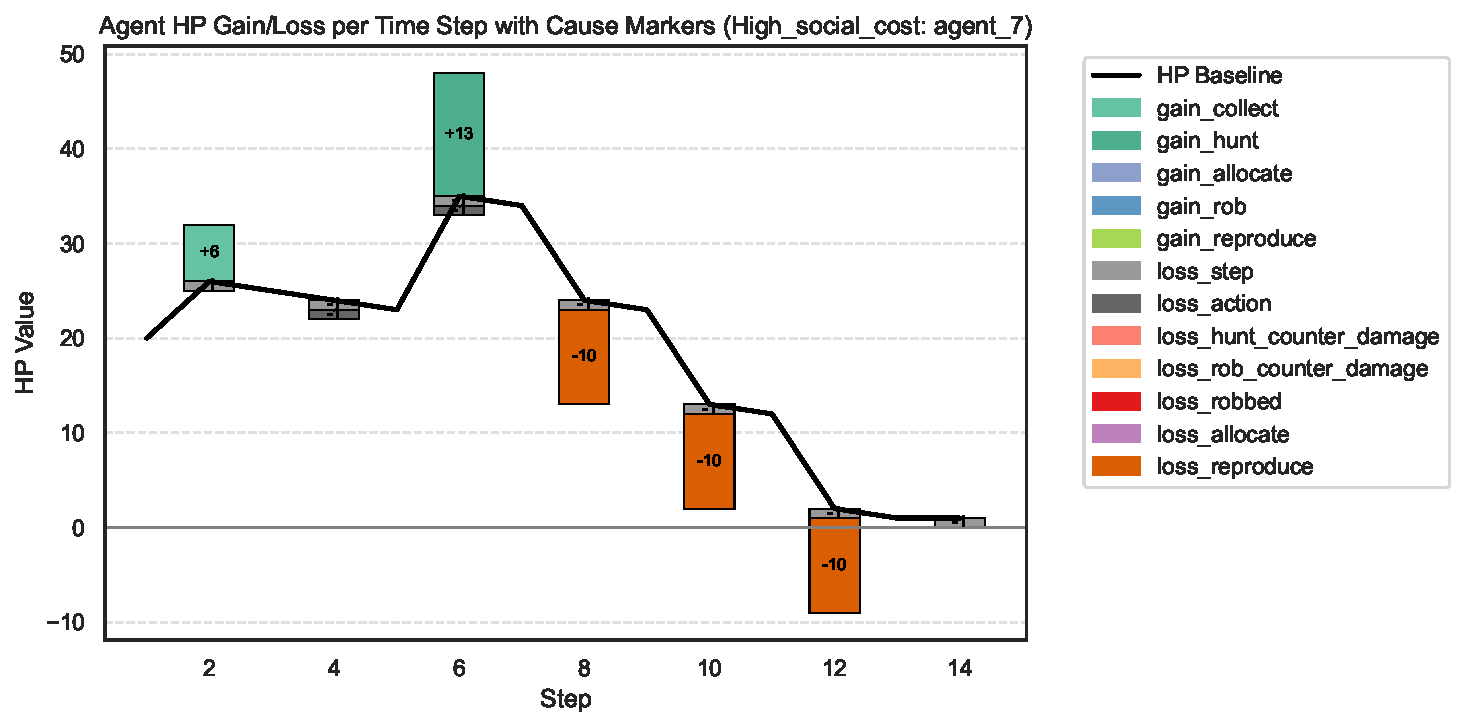
\includegraphics[width=\linewidth]{appendix_figures/HP/hp_change_High_social_cost_agent_7.pdf}
        \caption{HP and causes of an agent from an extinct type}
    \end{subfigure}
    \caption{Agent type ratio and count, and two example agent HP over time (Case: high social cost)}
    \label{fig:cost_pop}
\end{figure}

\textbf{Single Morality Scenarios}

Besides the simulations with various environment settings, we also conducted four experiments, where each experiment only had one single type of morality, with the baseline environment settings.

From the agent dynamics shown in Figure~\ref{fig:universal_pop},~\ref{fig:reciprocal_pop},~\ref{fig:kin_pop}, and~\ref{fig:selfish_pop}, agents have a high-reproduction period no matter morality types. After the first boom, universal moral agents and kin-focused agents maintain a relatively stable population, indicating that the resources are allocated fairly in general, but not high enough to reproduce. The reciprocal agents experience several oscillations, which may be because there are always agents gaining lots of resources when available to reproduce. Selfish agents are almost extinct after the boom, since they do not tend to collaborate to hunt when the plants are not available.
\begin{figure}[H]
    \centering
    \begin{subfigure}[t]{0.4\textwidth}
        \centering
        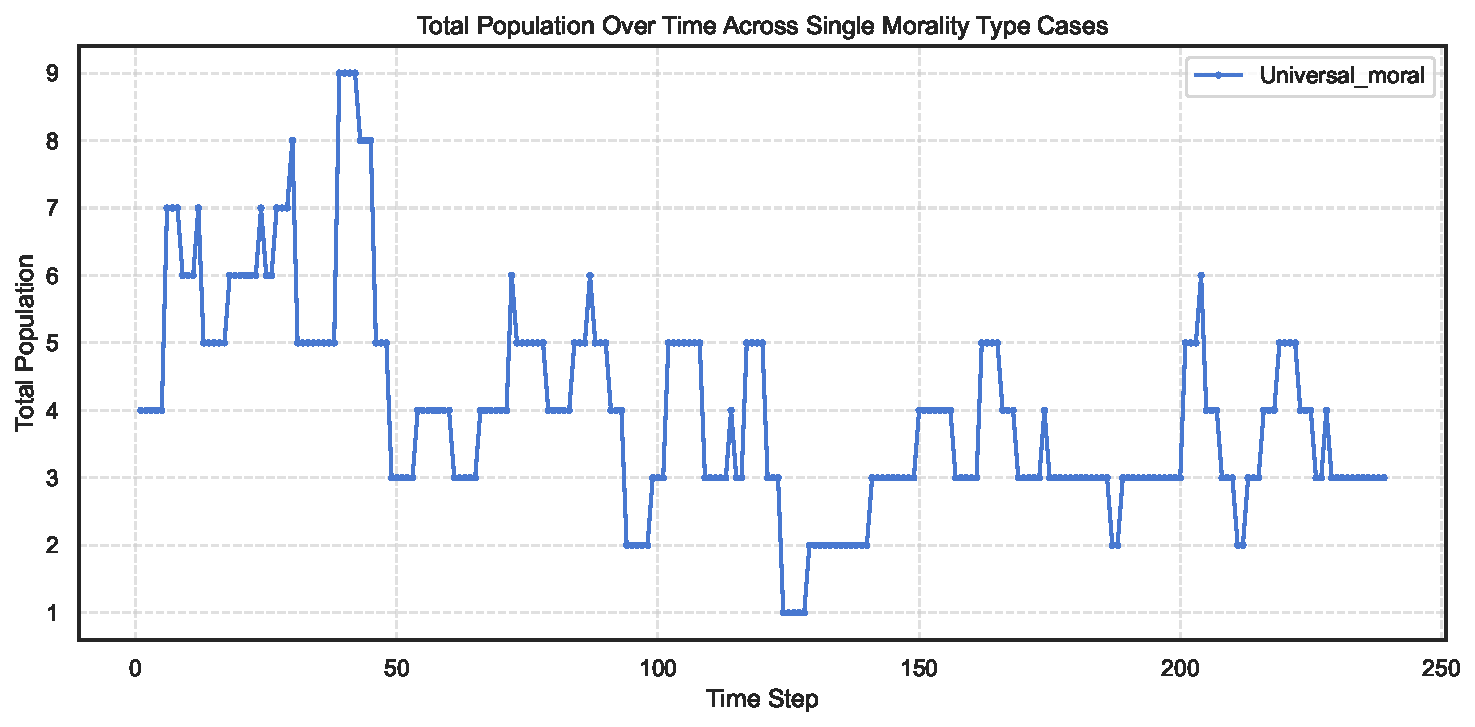
\includegraphics[width=\linewidth]{appendix_figures/populations/population_single_type_Universal_moral.pdf}
        \caption{Agent total count over time}
    \end{subfigure}
    \hfill
    
    \begin{subfigure}[t]{0.48\textwidth}
        \centering
        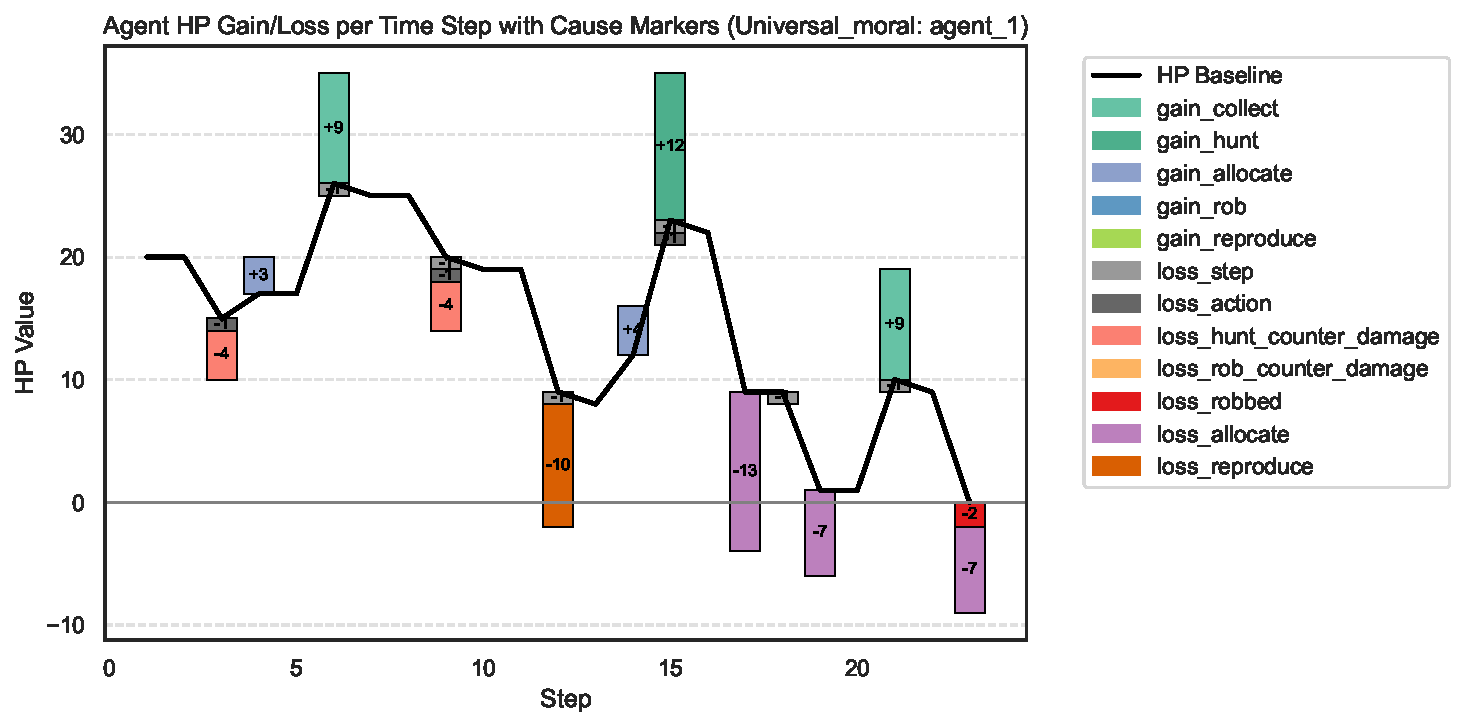
\includegraphics[width=\linewidth]{appendix_figures/HP/hp_change_Universal_moral_agent_1.pdf}
        \caption{HP and causes of an agent from a survival type}
    \end{subfigure}
    \hfill
    \begin{subfigure}[t]{0.48\textwidth}
        \centering
        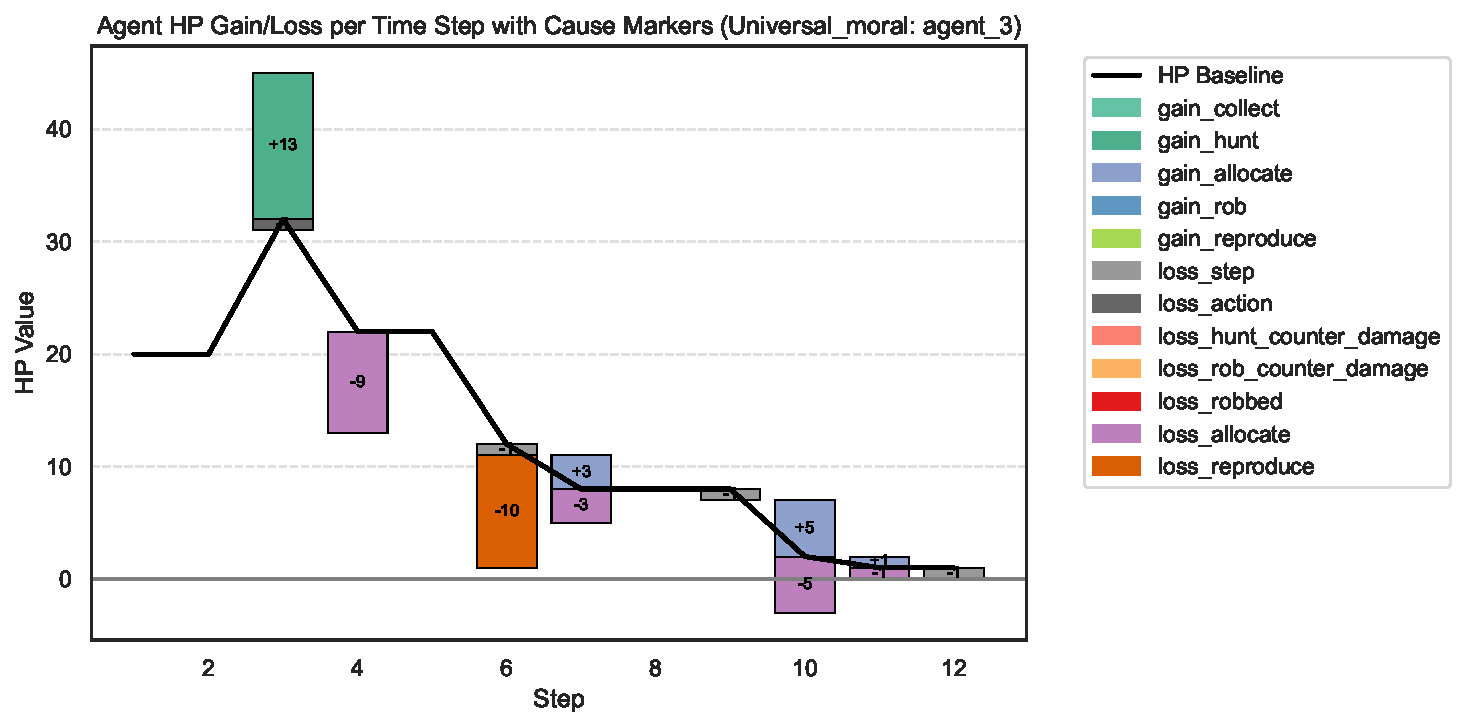
\includegraphics[width=\linewidth]{appendix_figures/HP/hp_change_Universal_moral_agent_3.pdf}
        \caption{HP and causes of an agent from an extinct type}
    \end{subfigure}
    \caption{Agent type ratio and count, and two example agent HP over time (Case:  universal type}
    \label{fig:universal_pop}
\end{figure}

\begin{figure}[H]
    \centering
    \begin{subfigure}[t]{0.4\textwidth}
        \centering
        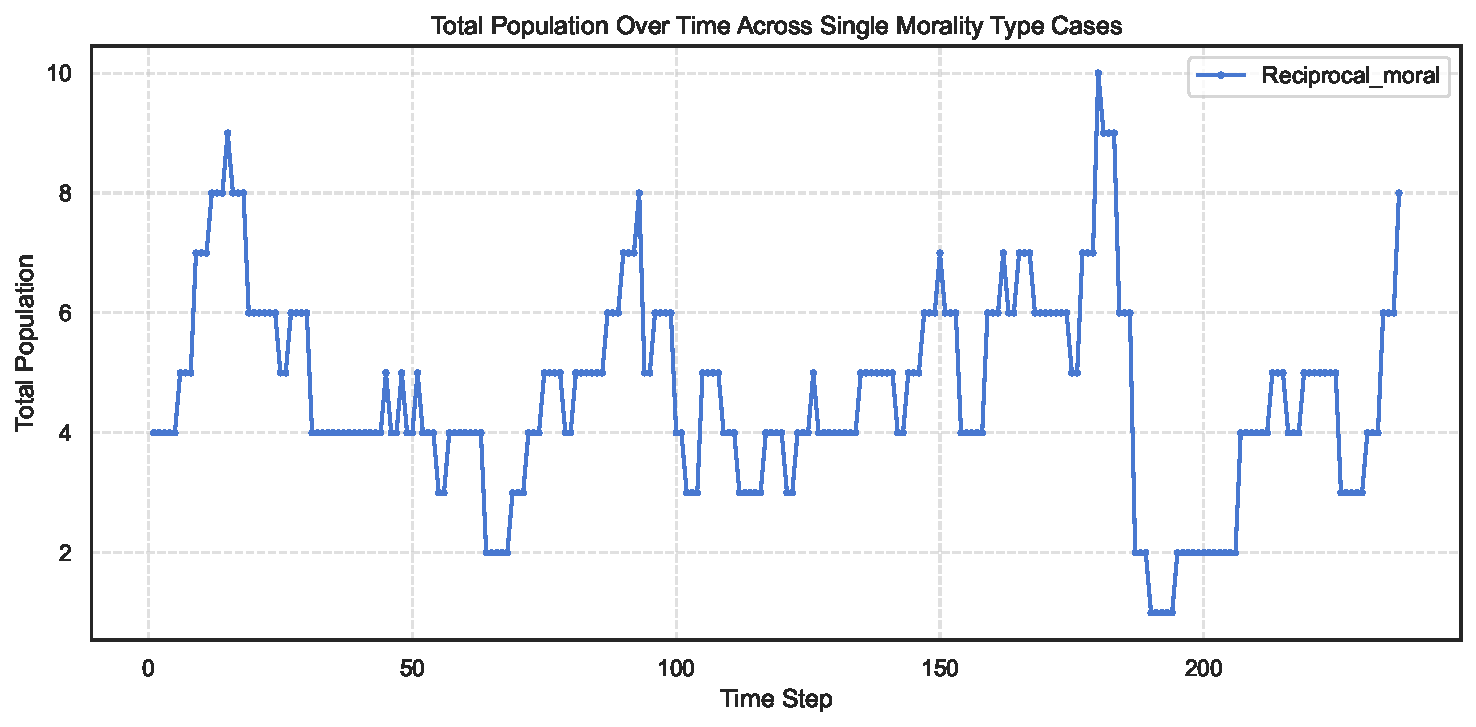
\includegraphics[width=\linewidth]{appendix_figures/populations/population_single_type_Reciprocal_moral.pdf}
        \caption{Agent total count over time}
    \end{subfigure}
    \hfill
    
    \begin{subfigure}[t]{0.48\textwidth}
        \centering
        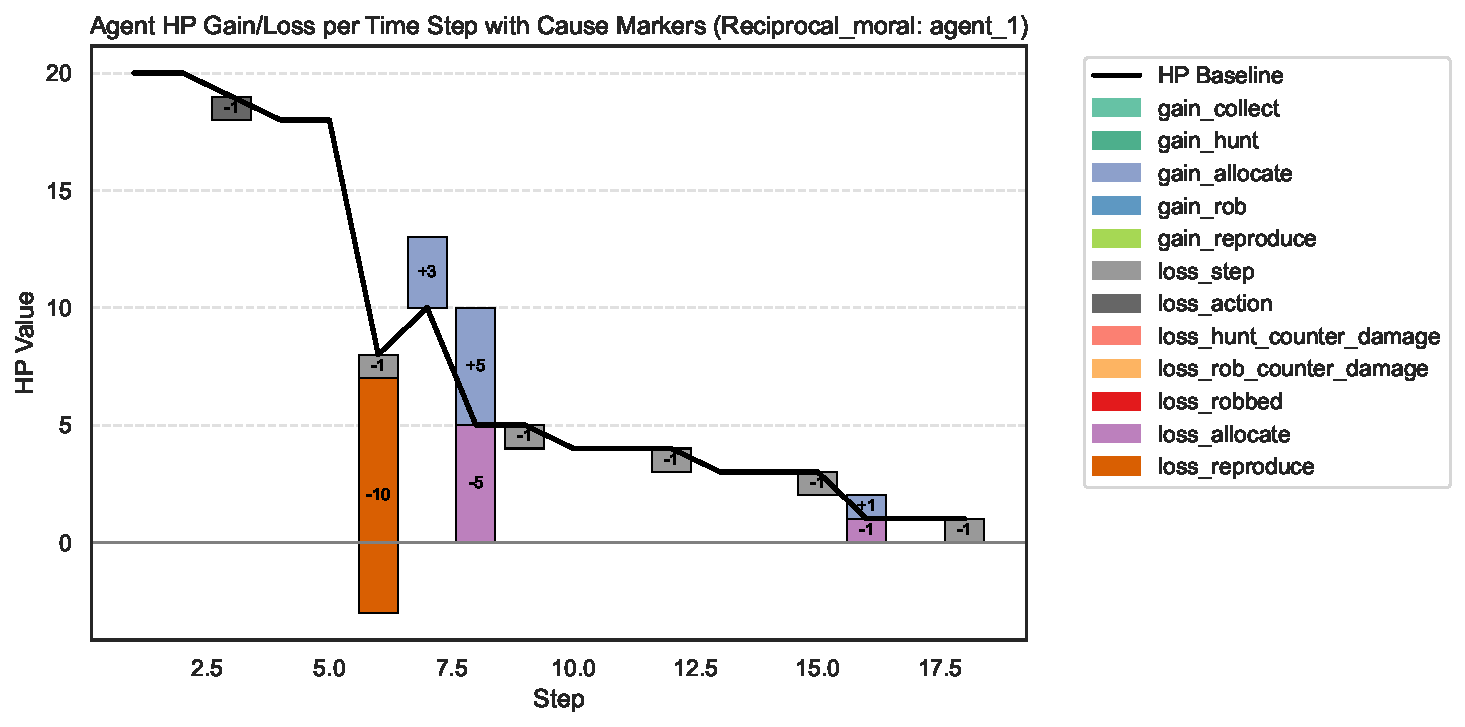
\includegraphics[width=\linewidth]{appendix_figures/HP/hp_change_Reciprocal_moral_agent_1.pdf}
        \caption{HP and causes of an agent from a survival type}
    \end{subfigure}
    \hfill
    \begin{subfigure}[t]{0.48\textwidth}
        \centering
        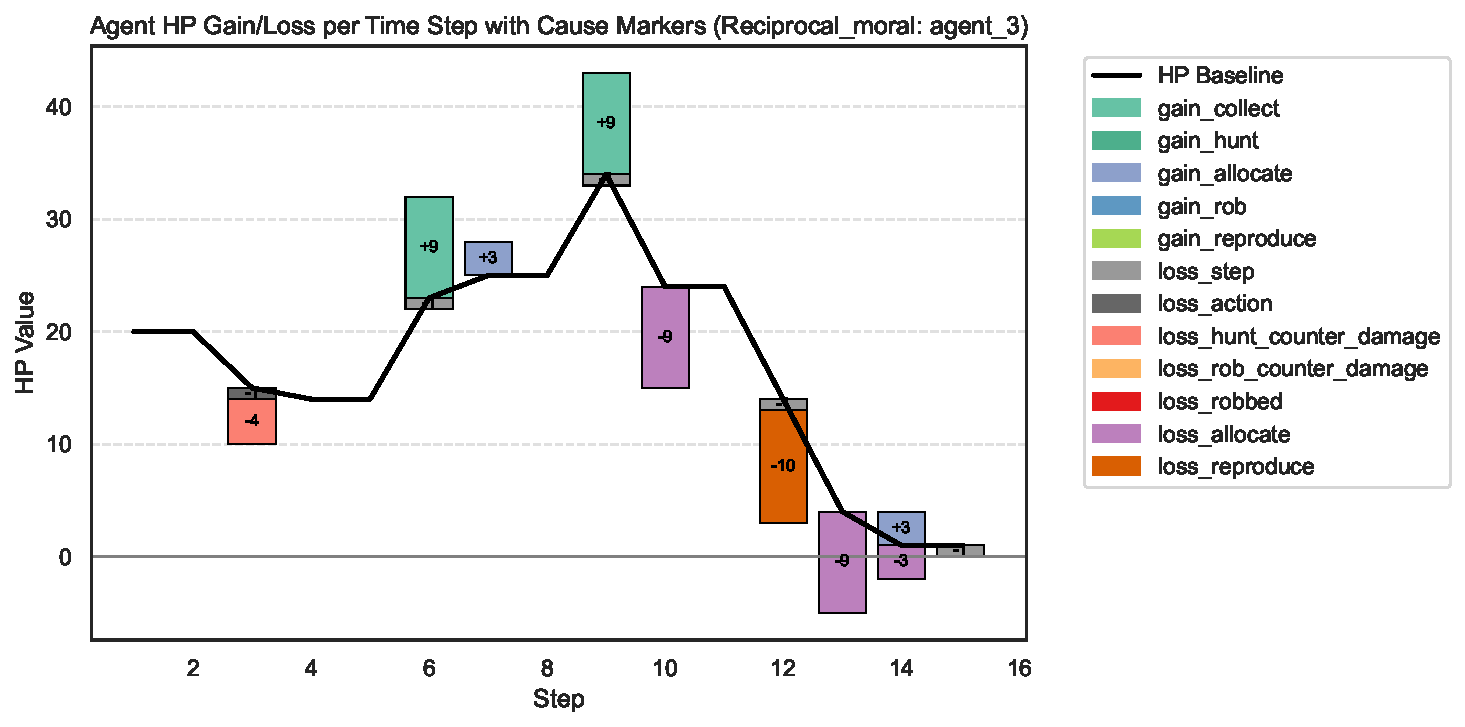
\includegraphics[width=\linewidth]{appendix_figures/HP/hp_change_Reciprocal_moral_agent_3.pdf}
        \caption{HP and causes of an agent from an extinct type}
    \end{subfigure}
    \caption{Agent type ratio and count, and two example agent HP over time (Case:  reciprocal type)}
    \label{fig:reciprocal_pop}
\end{figure}

\begin{figure}[H]
    \centering
    \begin{subfigure}[t]{0.4\textwidth}
        \centering
        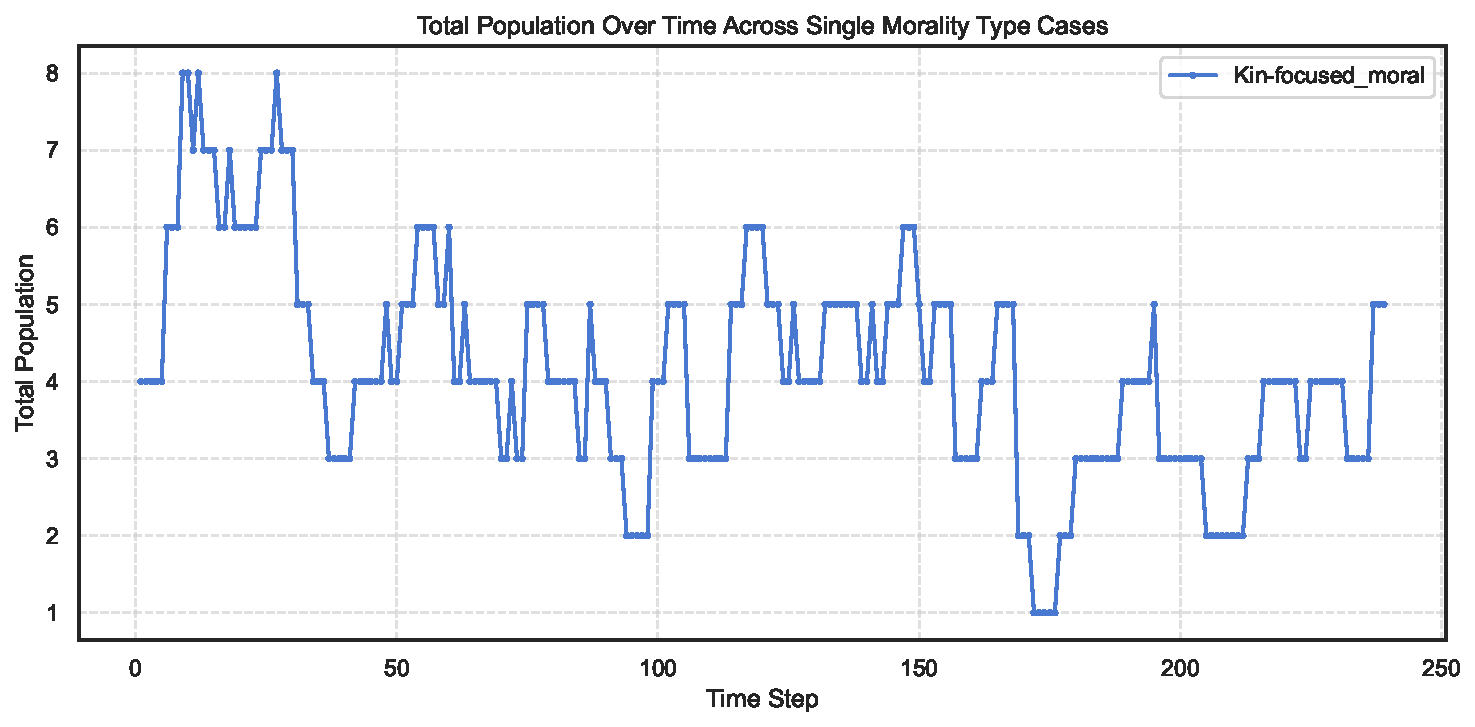
\includegraphics[width=\linewidth]{appendix_figures/populations/population_single_type_Kin-focused_moral.pdf}
        \caption{Agent total count over time}
    \end{subfigure}
    \hfill
    
    \begin{subfigure}[t]{0.48\textwidth}
        \centering
        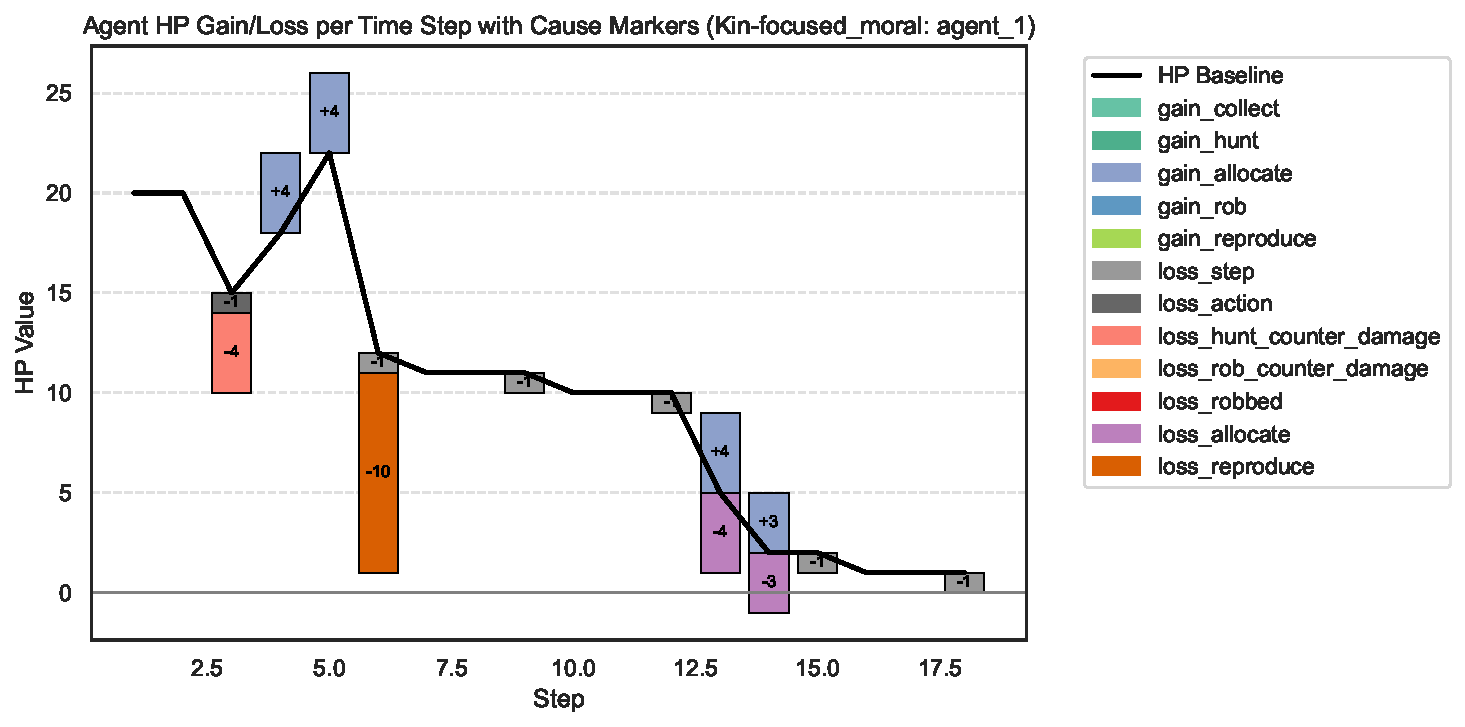
\includegraphics[width=\linewidth]{appendix_figures/HP/hp_change_Kin-focused_moral_agent_1.pdf}
        \caption{HP and causes of an agent from a survival type}
    \end{subfigure}
    \hfill
    \begin{subfigure}[t]{0.48\textwidth}
        \centering
        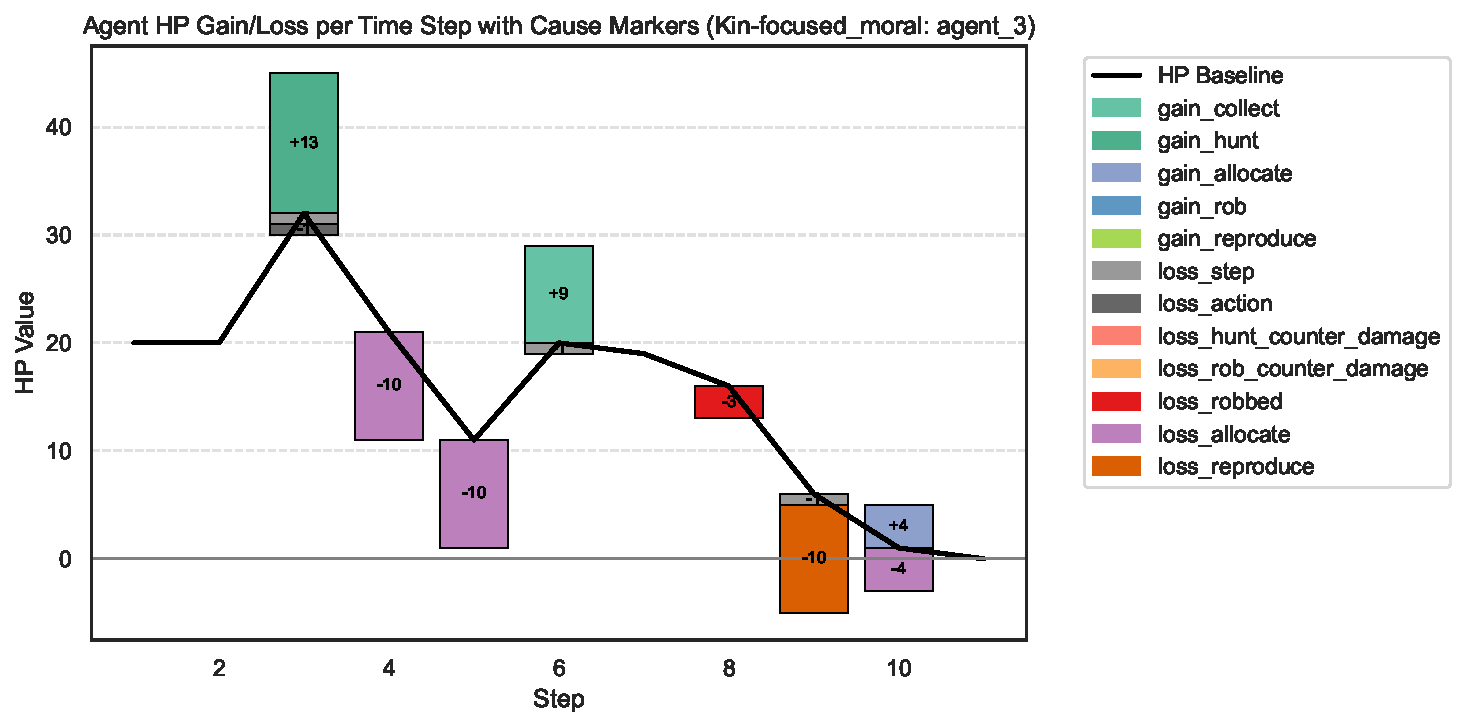
\includegraphics[width=\linewidth]{appendix_figures/HP/hp_change_Kin-focused_moral_agent_3.pdf}
        \caption{HP and causes of an agent from an extinct type}
    \end{subfigure}
    \caption{Agent type ratio and count, and two example agent HP over time (Case:  kin type)}
    \label{fig:kin_pop}
\end{figure}

\begin{figure}[H]
    \centering
    \begin{subfigure}[t]{0.4\textwidth}
        \centering
        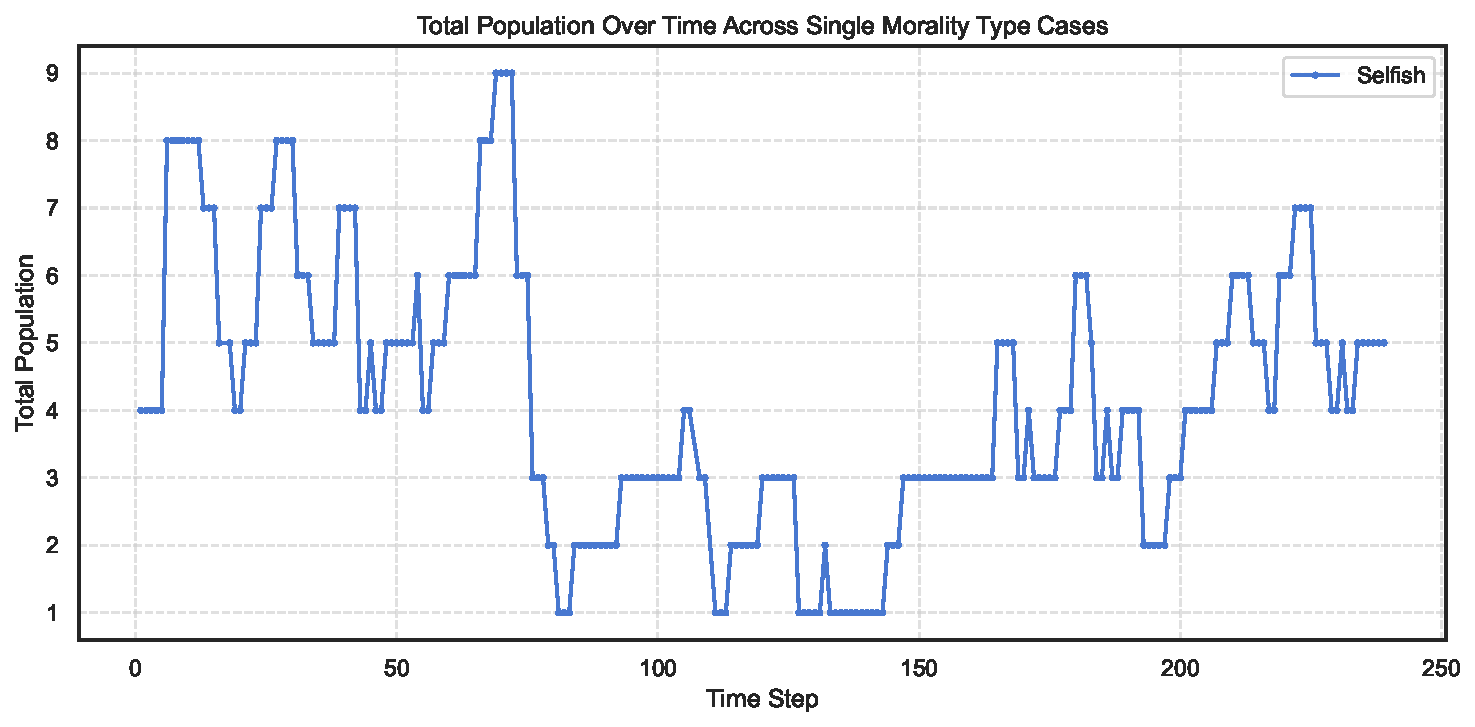
\includegraphics[width=\linewidth]{appendix_figures/populations/population_single_type_Selfish.pdf}
        \caption{Agent total count over time}
    \end{subfigure}
    \hfill
    
    \begin{subfigure}[t]{0.48\textwidth}
        \centering
        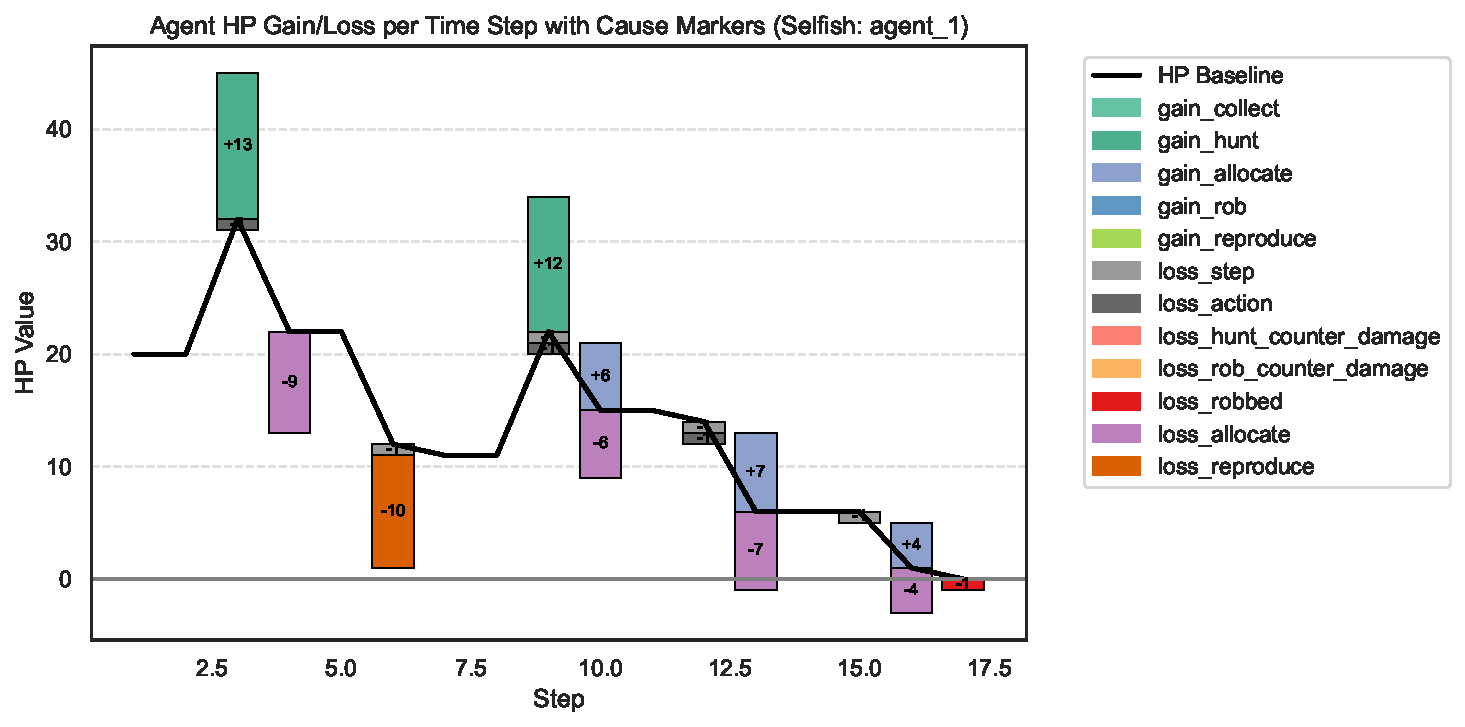
\includegraphics[width=\linewidth]{appendix_figures/HP/hp_change_Selfish_agent_1.pdf}
        \caption{HP and causes of an agent from a survival type}
    \end{subfigure}
    \hfill
    \begin{subfigure}[t]{0.48\textwidth}
        \centering
        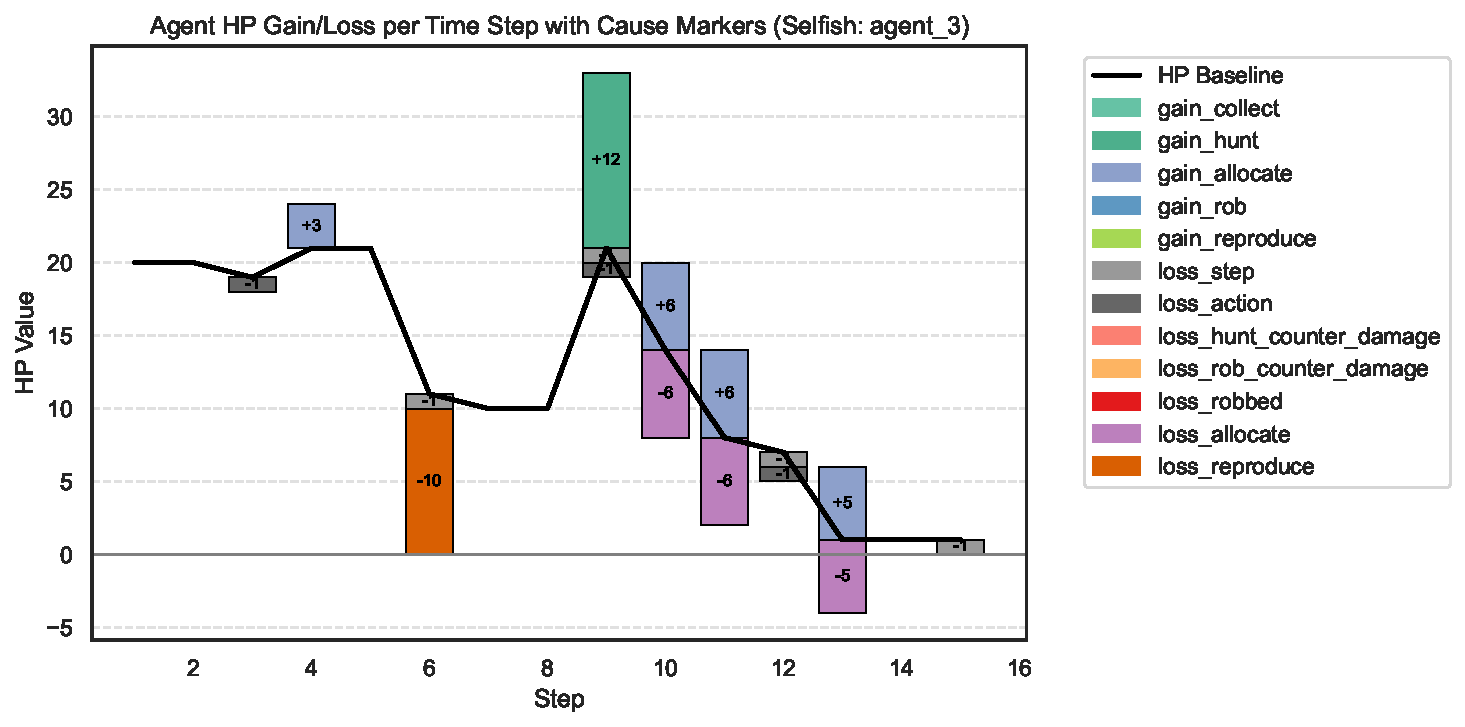
\includegraphics[width=\linewidth]{appendix_figures/HP/hp_change_Selfish_agent_3.pdf}
        \caption{HP and causes of an agent from an extinct type}
    \end{subfigure}
    \caption{Agent type ratio and count, and two example agent HP over time (Case:  selfish type)}
    \label{fig:selfish_pop}
\end{figure}

\subsubsection{Agents' lifespan}

The lifespan distributions of agents are visualized in Figures~\ref{fig: lifespan_main} to \ref{fig: lifespan_single}. Each figure is a histogram where the x-axis represents lifespan (in time steps), and the y-axis represents the frequency of agents. The bars indicate the count of agents with specific lifespans.

By comparing different settings with the baseline experiments, we could draw several conclusions, which are probably naive, but they validate our simulation:
\begin{itemize}
    \item Abundant resources increase the lifespan of agents, especially for selfish agents;
    \item Scarce resources give a higher variation of lifespan
    \item High social cost makes selfish agents difficult to pass the baby period
    \item Invisible morality balances the lifespan of the different moral agents
\end{itemize}


\begin{figure}[H]
    \centering
        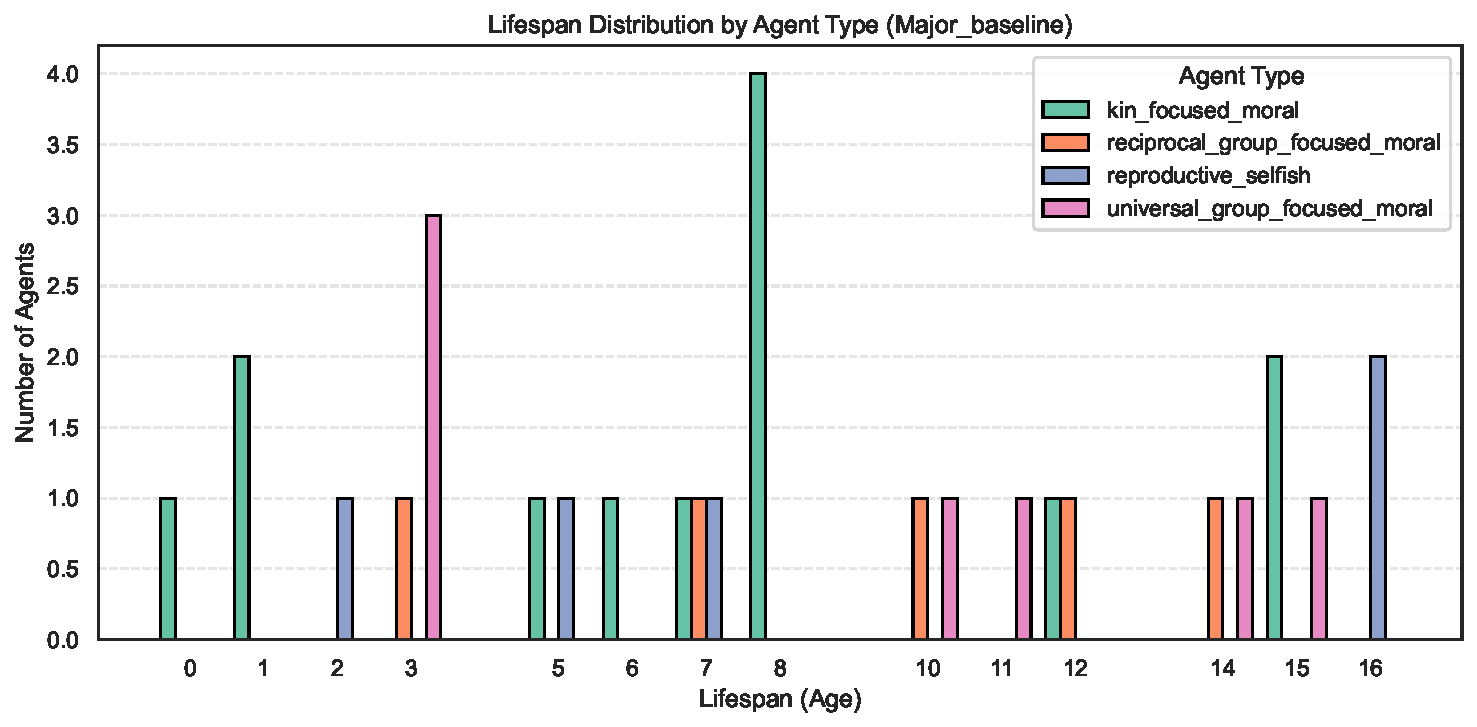
\includegraphics[width=0.85\columnwidth]{appendix_figures/lifespan/lifespan_distribution_Major_baseline.pdf}
        \caption{Lifespan Distribution by Agent Type (Case: Major baseline)}
        \label{fig: lifespan_main}
\end{figure}
    
\begin{figure}[H]
        \centering
        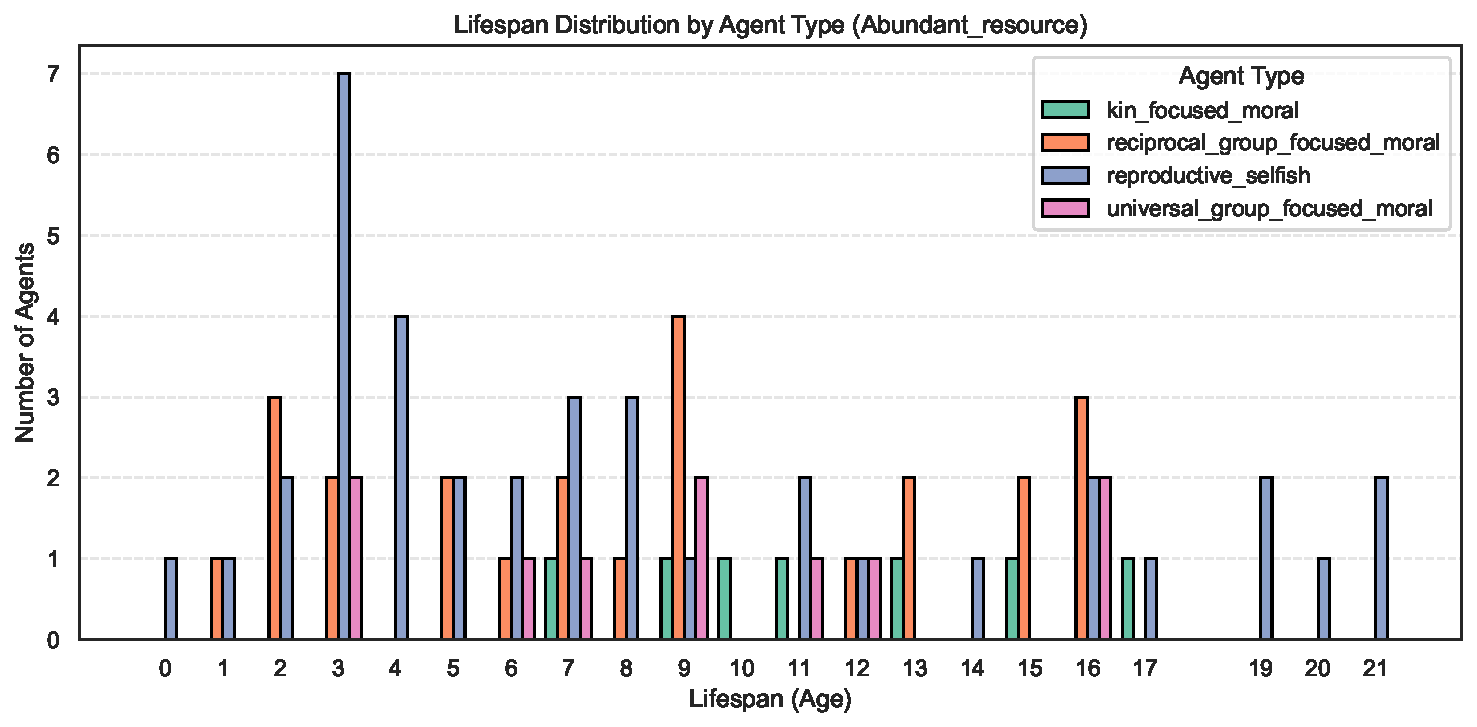
\includegraphics[width=0.85\columnwidth]{appendix_figures/lifespan/lifespan_distribution_Abundant_resource.pdf}
        \caption{Lifespan Distribution by Agent Type (Case: Abundant resource)}
        \label{fig: lifespan_abundant}
\end{figure}
    
\begin{figure}[H]
    \centering
        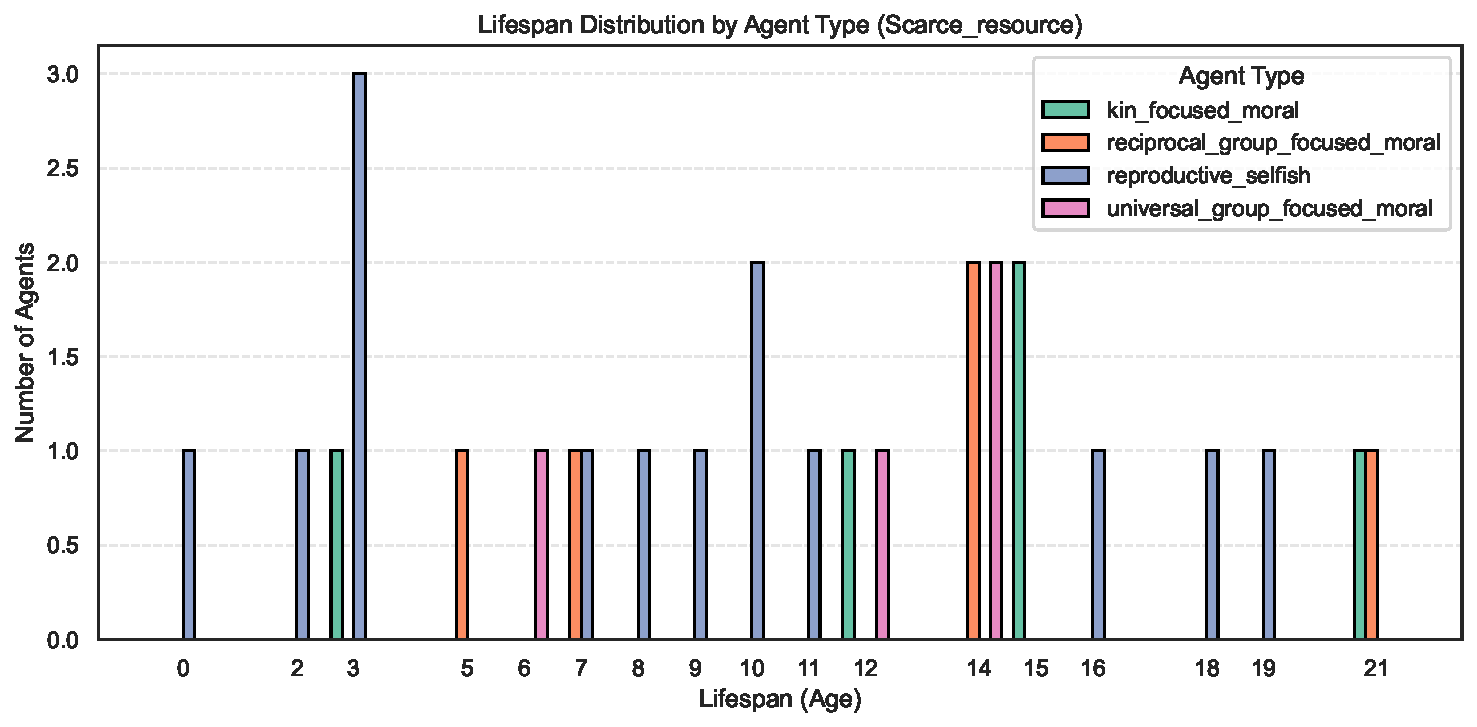
\includegraphics[width=0.85\columnwidth]{appendix_figures/lifespan/lifespan_distribution_Scarce_resource.pdf}
        \caption{Lifespan Distribution by Agent Type (Case: Scarce resource)}
        \label{fig: lifespan_scarce}
\end{figure}

\begin{figure}[H]
    \centering
        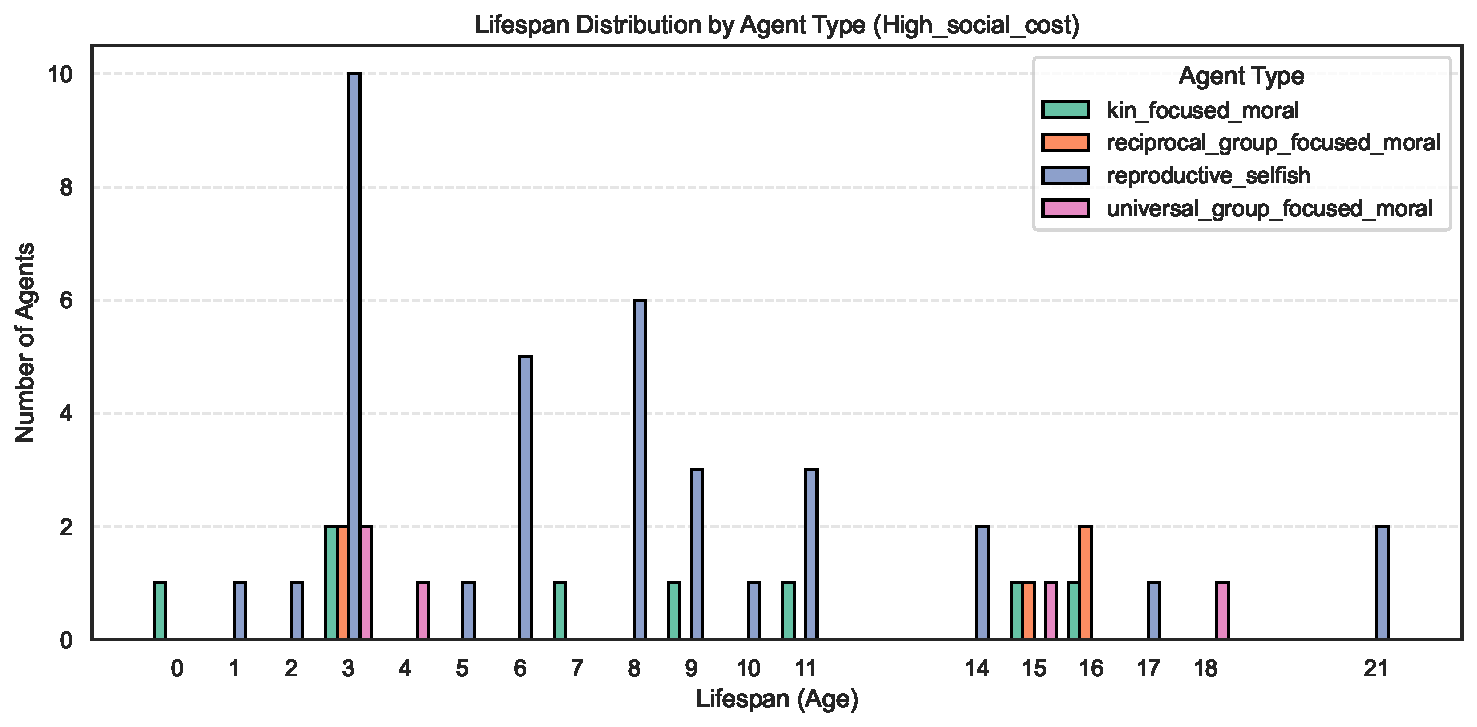
\includegraphics[width=0.85\columnwidth]{appendix_figures/lifespan/lifespan_distribution_High_social_cost.pdf}
        \caption{Lifespan Distribution by Agent Type (Case: High social cost)}
    \label{fig: lifespan_social_cost}
\end{figure}

\begin{figure}[H]
    \centering
        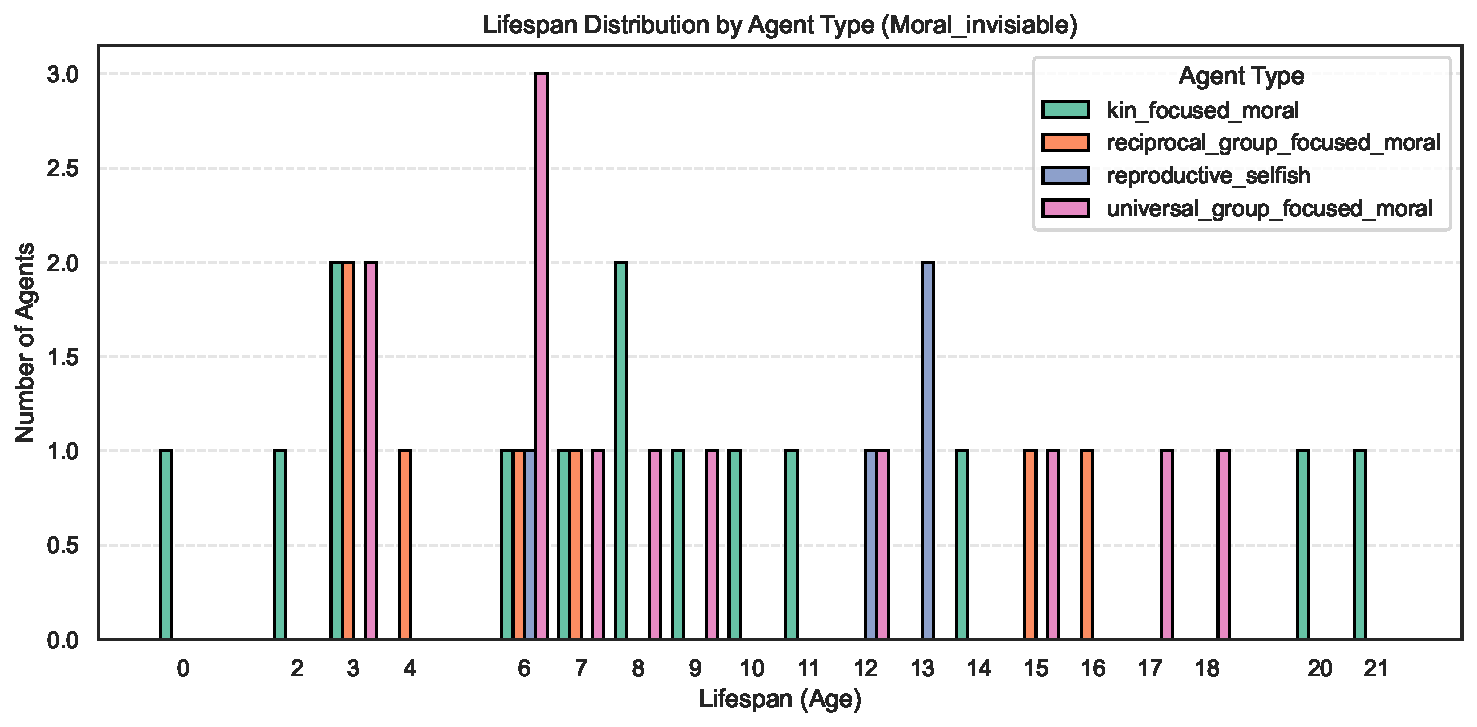
\includegraphics[width=0.85\columnwidth]{appendix_figures/lifespan/lifespan_distribution_Moral_invisiable.pdf}
    \caption{Lifespan Distribution by Agent Type (Case: Moral invisible)}
    \label{fig: lifespan_invi}
\end{figure}

\begin{figure}[H]
    \centering
    \begin{subfigure}[t]{0.45\columnwidth}
        \centering
        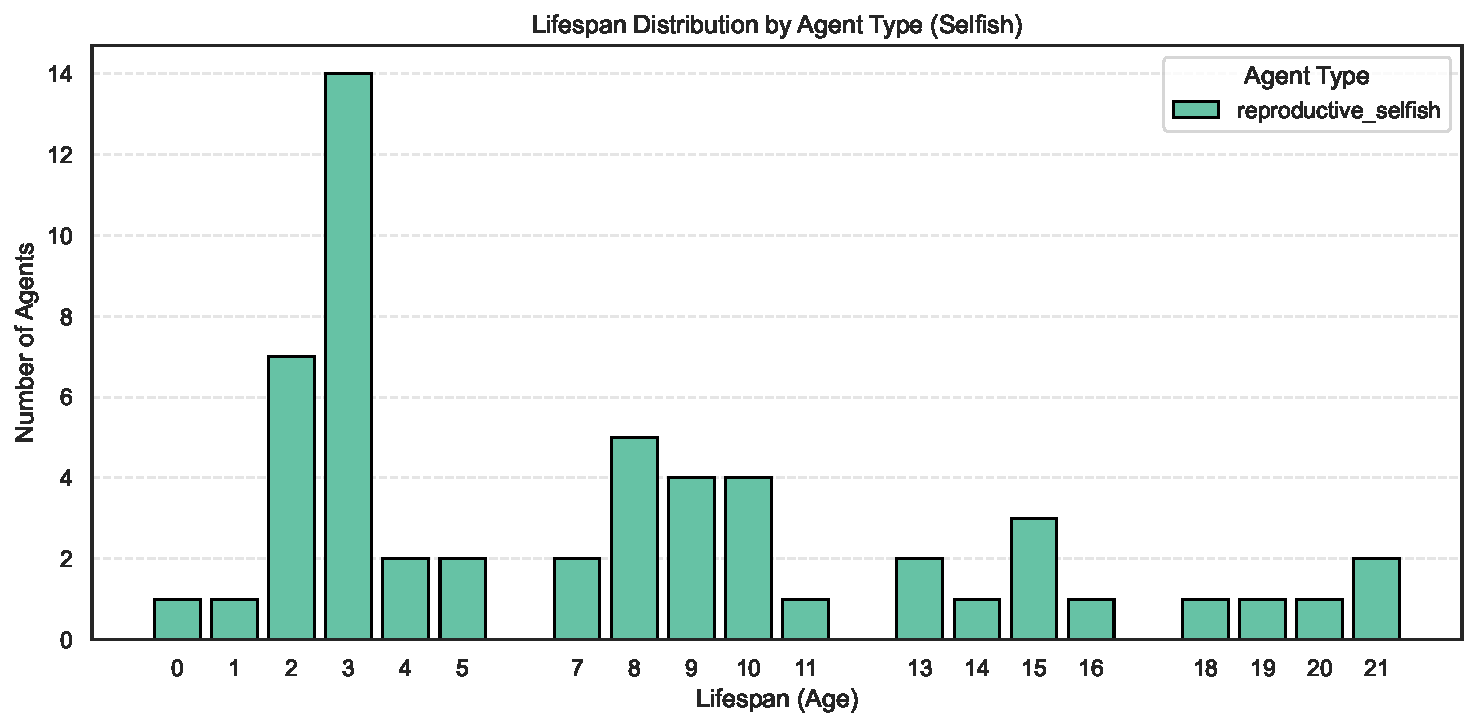
\includegraphics[width=\linewidth]{appendix_figures/lifespan/lifespan_distribution_Selfish.pdf}
        \caption{Lifespan Distribution by Agent Type (Case: Selfish)}
    \end{subfigure}
    \hfill
    \begin{subfigure}[t]{0.45\columnwidth}
        \centering
        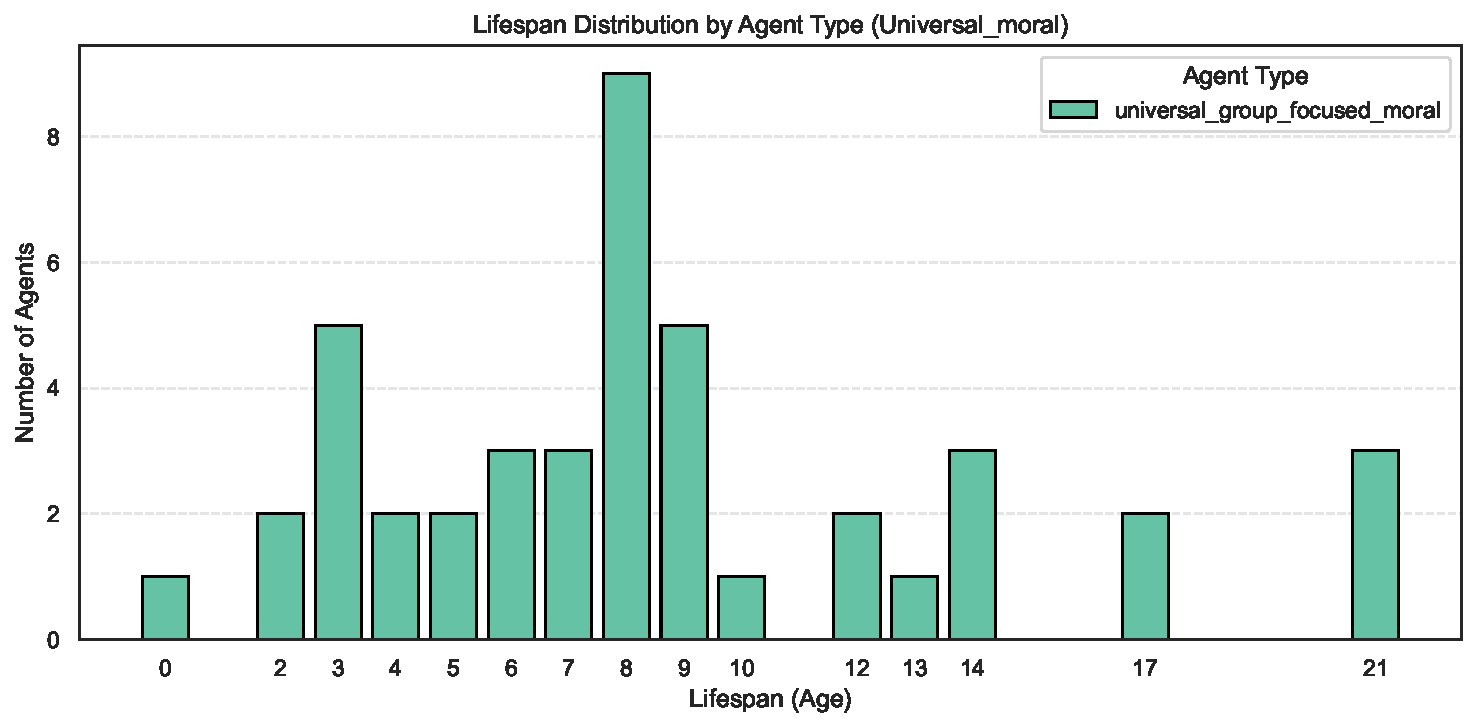
\includegraphics[width=\linewidth]{appendix_figures/lifespan/lifespan_distribution_Universal_moral.pdf}
        \caption{Lifespan Distribution by Agent Type (Case: Universal)}
    \end{subfigure}
    \hfill
    
    \begin{subfigure}[t]{0.45\columnwidth}
        \centering
        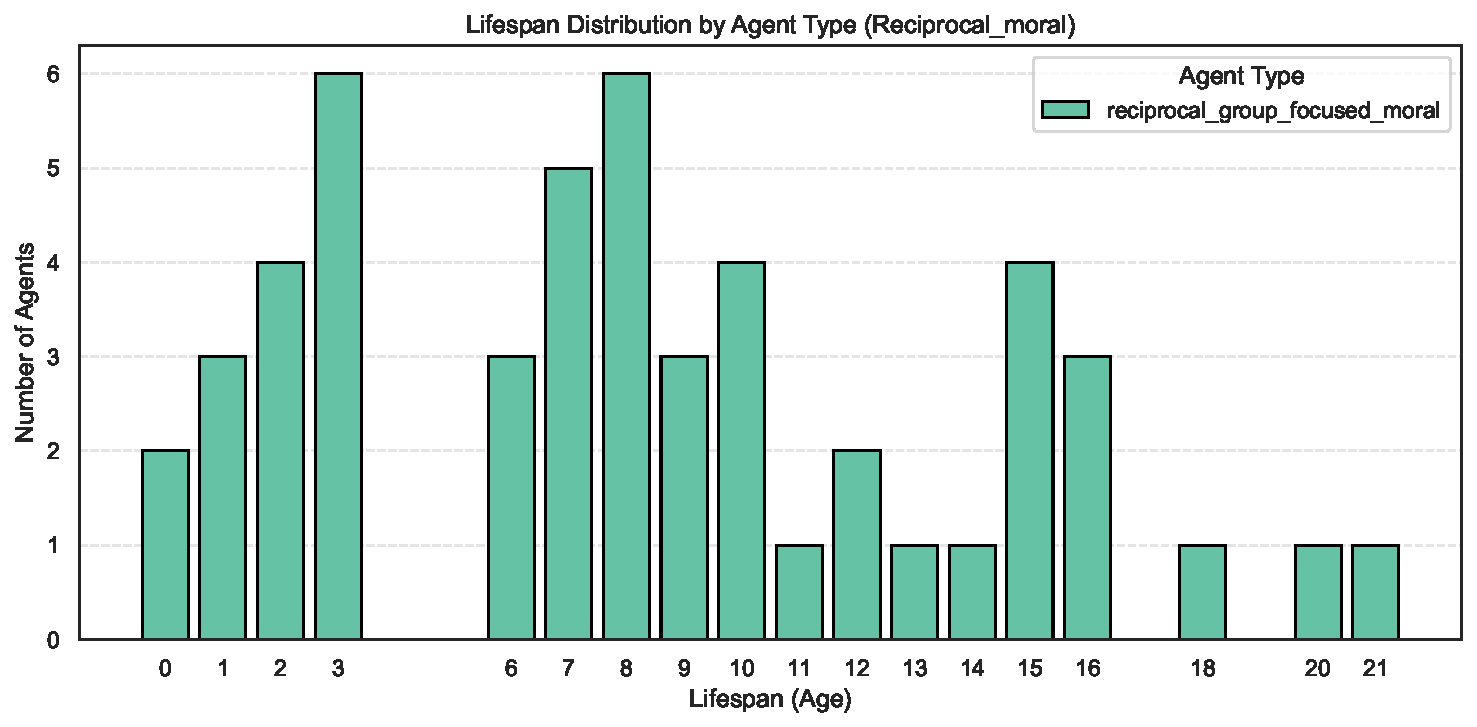
\includegraphics[width=\linewidth]{appendix_figures/lifespan/lifespan_distribution_Reciprocal_moral.pdf}
        \caption{Lifespan Distribution by Agent Type (Case: reciprocal)}
    \end{subfigure}
    \hfill
    \begin{subfigure}[t]{0.45\columnwidth}
        \centering
        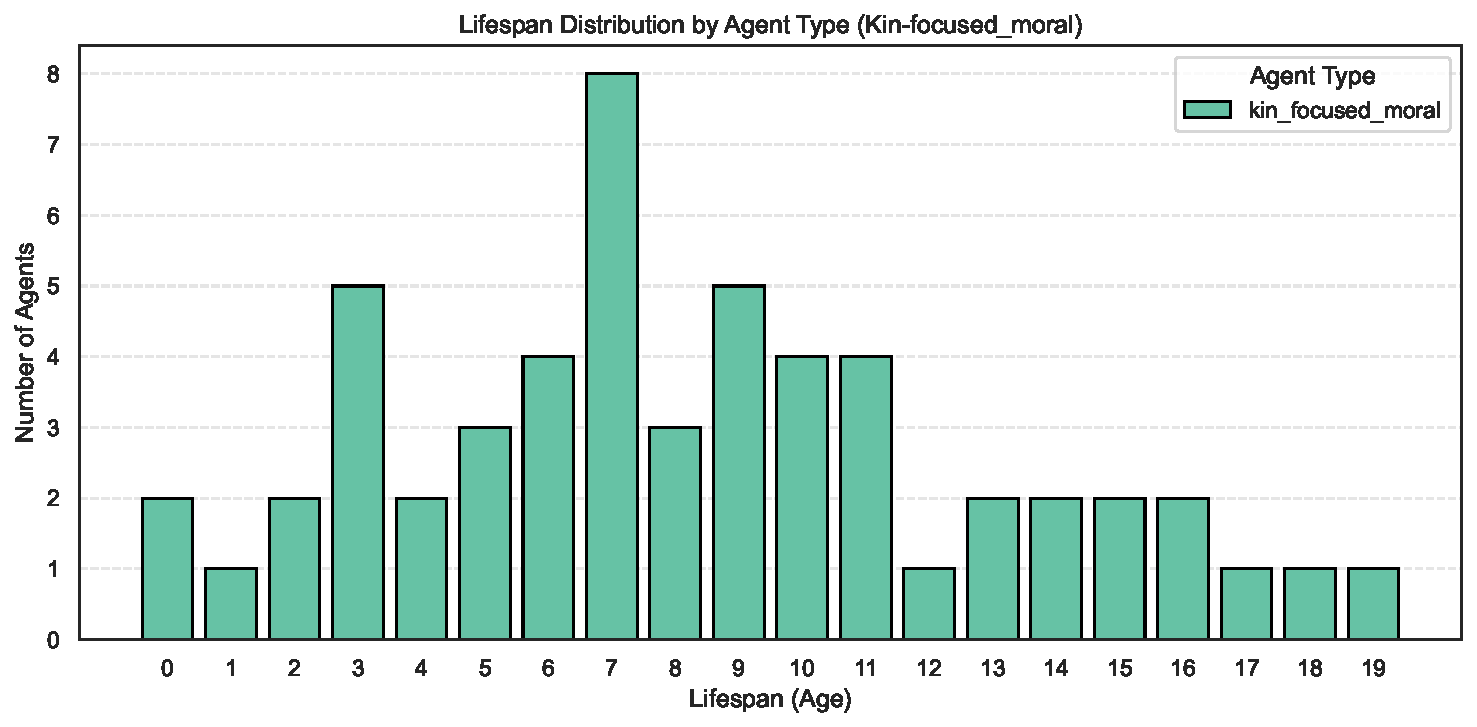
\includegraphics[width=\linewidth]{appendix_figures/lifespan/lifespan_distribution_Kin-focused_moral.pdf}
        \caption{Lifespan Distribution by Agent Type (Case: kin)}
    \end{subfigure}

    \caption{Lifespan Distribution for tests under single Agent Type settings}
    \label{fig: lifespan_single}
\end{figure}


\subsubsection{Action distributions for each experiment}

Figure~\ref{fig: action type proportion1} and~\ref{fig: action type proportion2} present the proportions of action types across different test cases and agent morality types. Each subfigure is a bar chart where the x-axis represents action types (e.g., hunting, resting, social interactions), and the y-axis represents the proportion of actions.
This section examines the proportion of action types across test cases and agent morality types. Figures include:
1) Overall Action Proportions: Bar charts showing the percentage of each action type (e.g., hunting, resting, social interactions) across all test cases.
2) Action Proportions by Moral Type: Separate bar charts for Universal, Reciprocal, Kin-focused, and Selfish agents, highlighting their behavioral tendencies across scenarios.

From the figure, we could observe that:
\begin{itemize}
    \item Only selfish agents have taken the ``rob" action, and they do not like ``communicate" and ``allocate"
    \item ``Collect" actions are taken mostly when resources are abundant, no matter what morality is
    \item When social cost is high, agents tend to ``reproduce" more than in other settings
\end{itemize}


\begin{figure}[H]
    \centering
    % 第一行：3张图
    % \begin{subfigure}[t]{0.85\columnwidth}
    %     \centering
    %     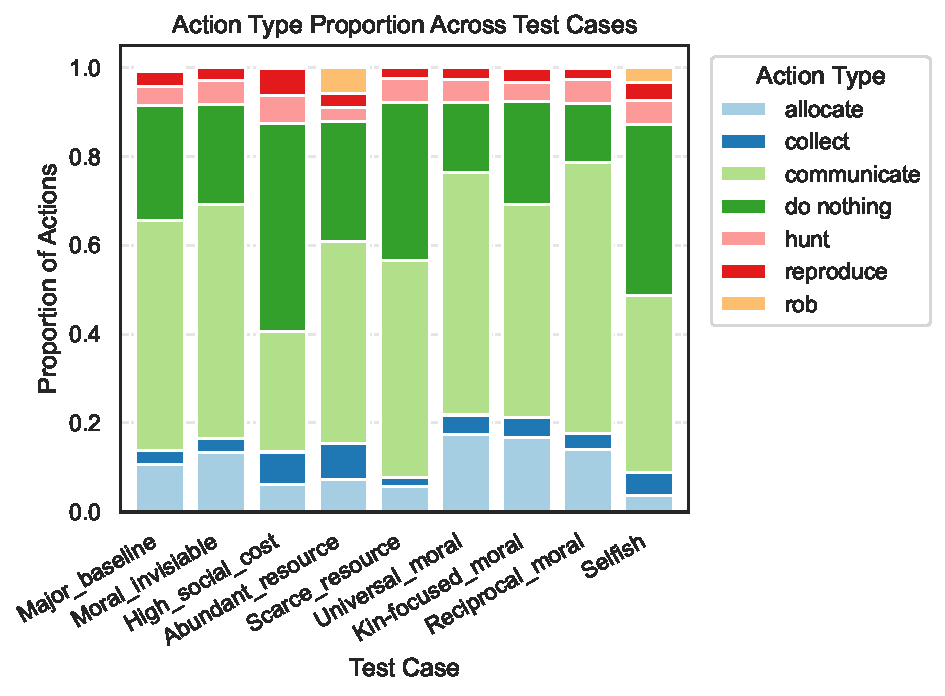
\includegraphics[width=\linewidth]{appendix_figures/actions/action_distribution_across_cases.pdf}
    %     \caption{Action type proportion across test cases}
    % \end{subfigure}
    % \hfill
    
    \begin{subfigure}[t]{0.45\columnwidth}
        \centering
        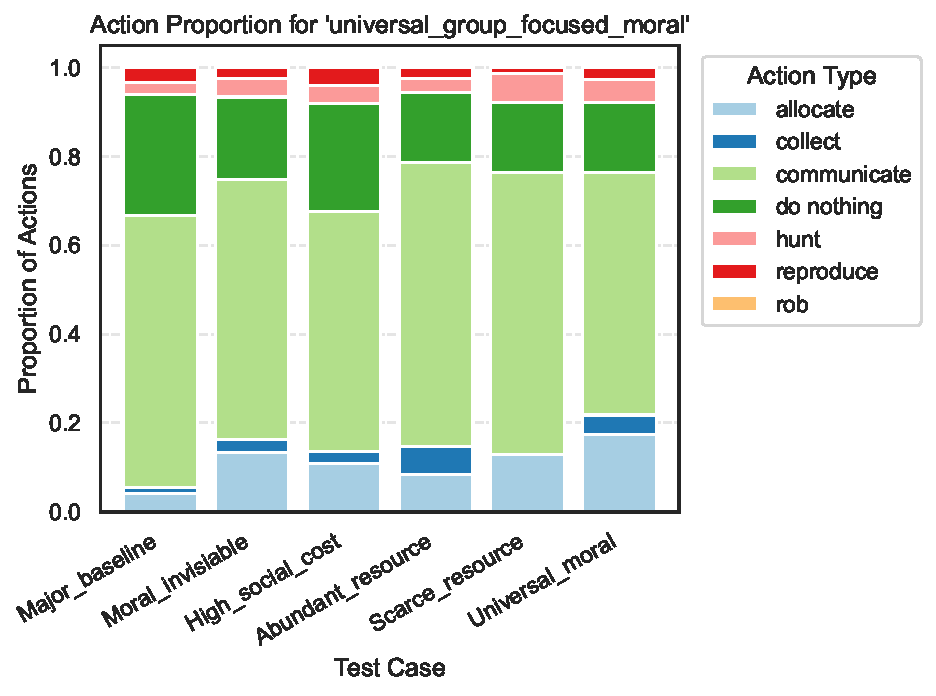
\includegraphics[width=\linewidth]{appendix_figures/actions/action_distr_across_cases_universal_group_focused_moral.pdf}
        \caption{Action Type Proportion for universal moral agents}
    \end{subfigure}
    \hfill
    \begin{subfigure}[t]{0.45\columnwidth}
        \centering
        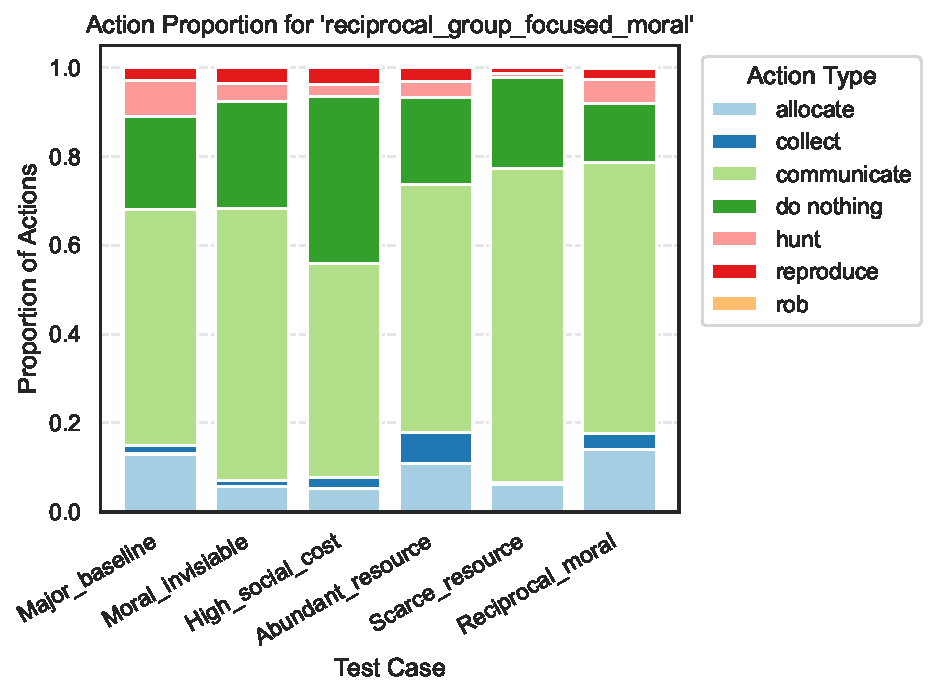
\includegraphics[width=\linewidth]{appendix_figures/actions/action_distr_across_cases_reciprocal_group_focused_moral.pdf}
        \caption{Action Type Proportion for reciprocal moral agents}
    \end{subfigure}
    \caption{Action type proportion across test cases and agent morality type}
    \label{fig: action type proportion1}
\end{figure}

\begin{figure}[H]
    \centering
    % 第二行：2张图，居中
    \begin{subfigure}[t]{0.45\columnwidth}
        \centering
        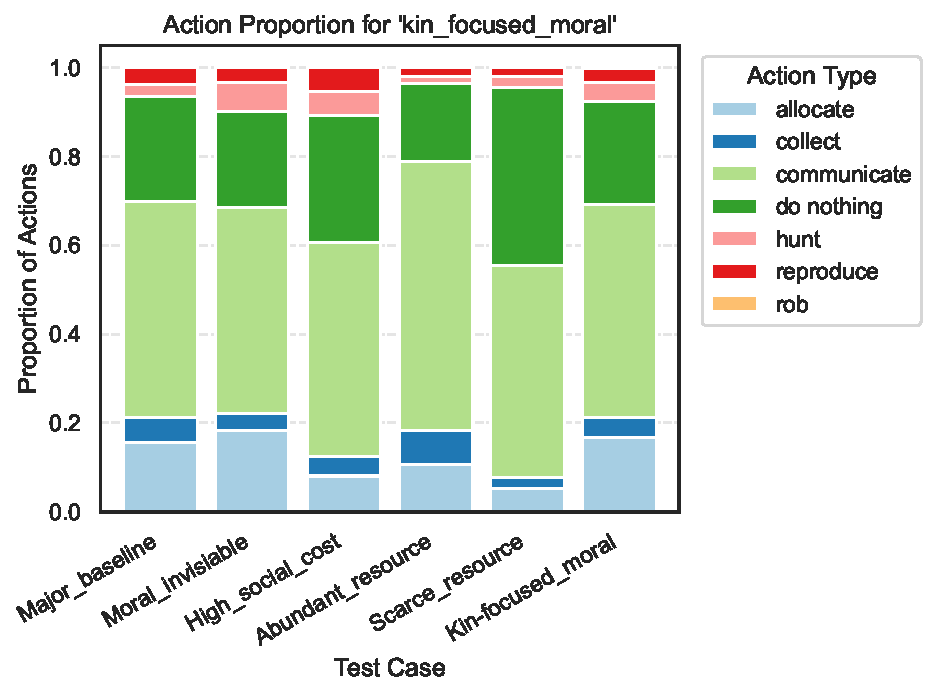
\includegraphics[width=\linewidth]{appendix_figures/actions/action_distr_across_cases_kin_focused_moral.pdf}
        \caption{Action Type Proportion for kin-focused moral agents}
    \end{subfigure}
    \hfill  % 中间空隙控制居中
    \begin{subfigure}[t]{0.45\columnwidth}
        \centering
        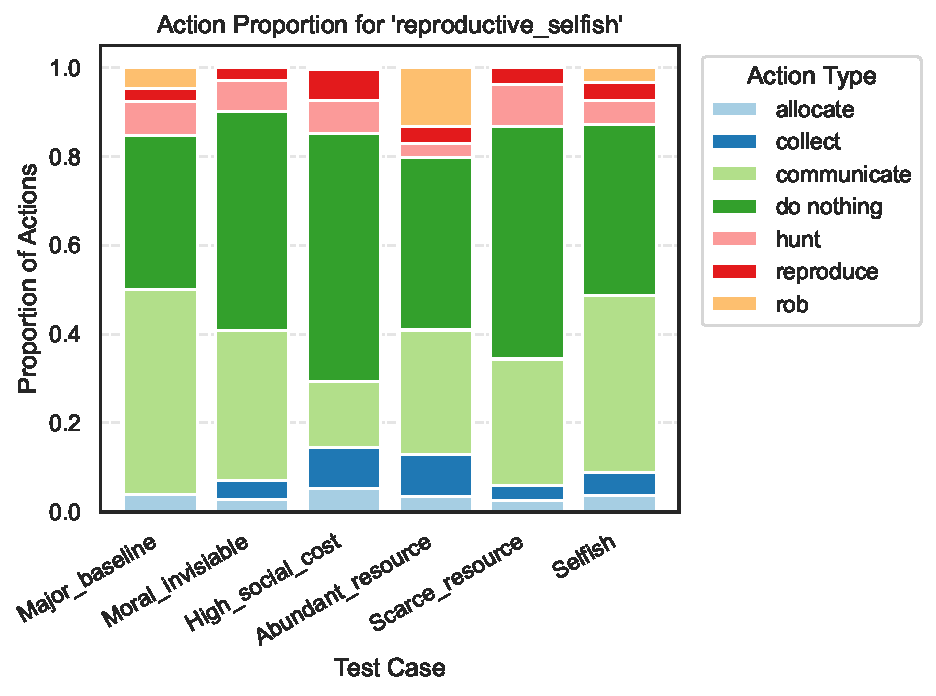
\includegraphics[width=\linewidth]{appendix_figures/actions/action_distr_across_cases_reproductive_selfish.pdf}
        \caption{Action Type Proportion for selfish agents}
    \end{subfigure}

    \caption{Action type proportion across test cases and agent morality type}
    \label{fig: action type proportion2}
\end{figure}


\subsubsection{Action distributions for each moral type}

Figures~\ref{fig: actions_type_main} to \ref{fig: actions_type_selfish} detail the mean actions initiated and received by agents of each moral type. Each figure consists of two bar charts:
\begin{itemize}
    \item The first chart shows the mean actions initiated per agent, with the x-axis representing action types and the y-axis representing the average number of actions initiated.
    \item The second chart shows the mean actions received per agent, with the x-axis representing action types and the y-axis representing the average number of actions received.
\end{itemize}

From all these figures, we could conclude that:
\begin{itemize}
    \item Selfish agents receive the least communications and allocations
    \item Universal moral and kin-focused moral initiate the most allocation
    \item Action variations are large, indicating the instability of the LLM inference
\end{itemize}

\begin{figure}[H]
    \centering
    \begin{subfigure}[t]{0.48\textwidth}
        \centering
        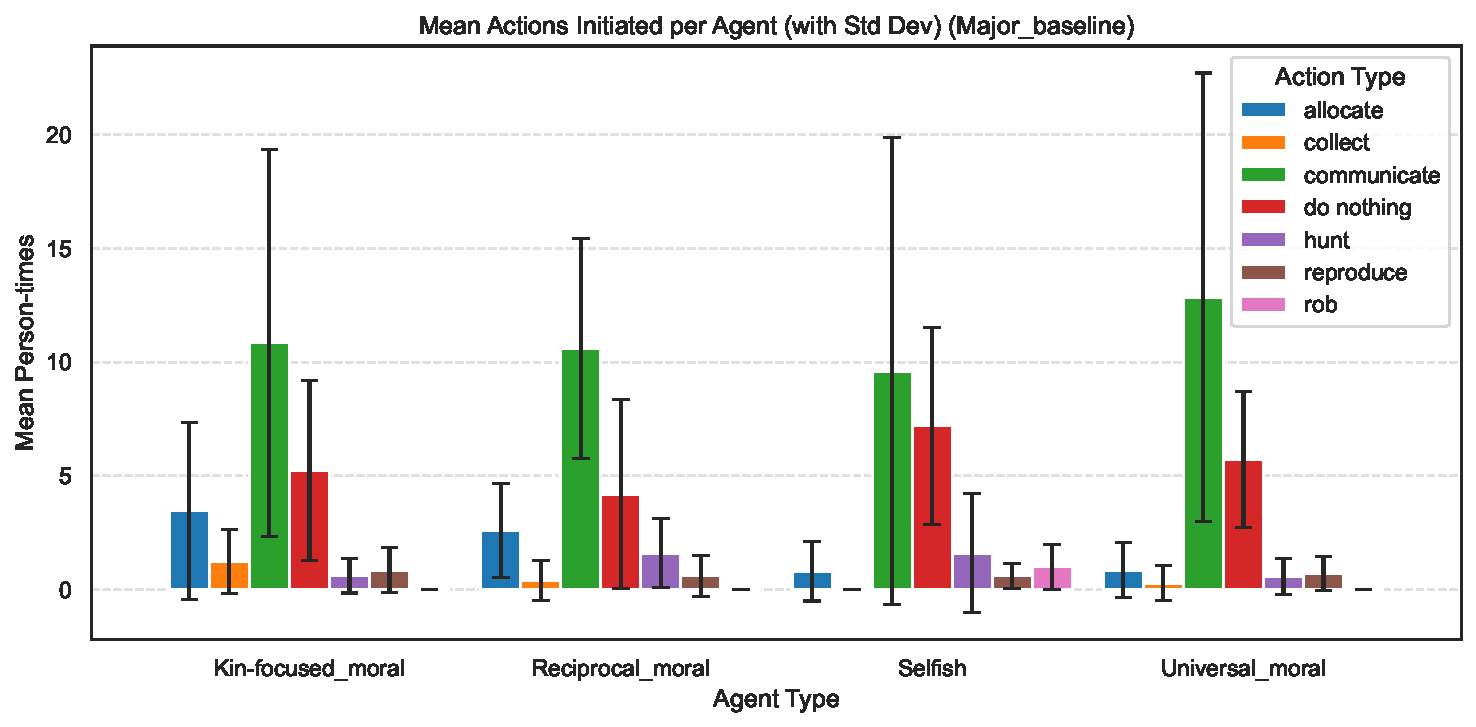
\includegraphics[width=\linewidth]{appendix_figures/actions/action_distri_initiator_by_type_Major_baseline.pdf}
        \caption{Mean Actions Initiated per Agent}
    \end{subfigure}
    \hfill
    \begin{subfigure}[t]{0.48\textwidth}
        \centering
        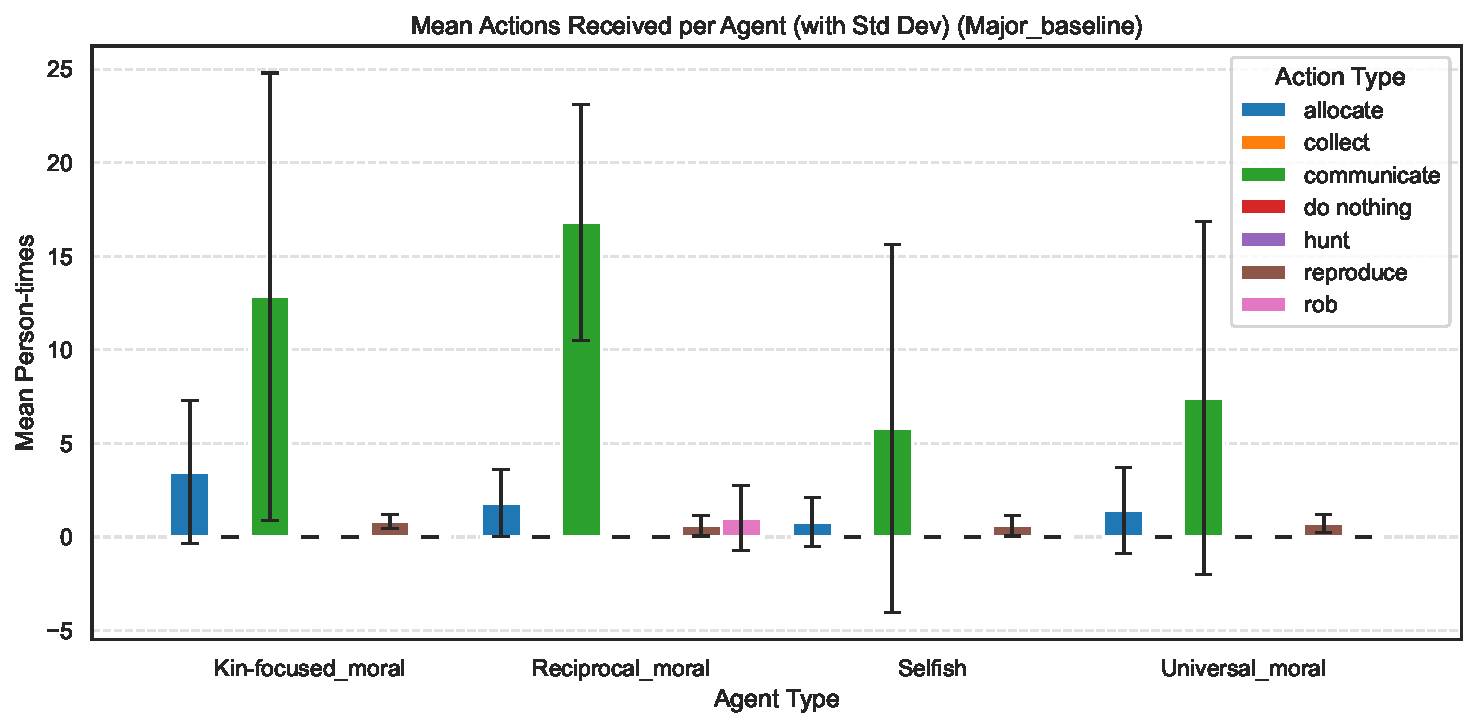
\includegraphics[width=\linewidth]{appendix_figures/actions/action_distri_receiver_by_type_Major_baseline.pdf}
        \caption{Mean Actions Received per Agent}
    \end{subfigure}
    \caption{Agent-times of action type when agents are initiators and receivers (Case: major baseline)}
    \label{fig: actions_type_main}
\end{figure}

\begin{figure}[H]
    \centering
    \begin{subfigure}[t]{0.48\textwidth}
        \centering
        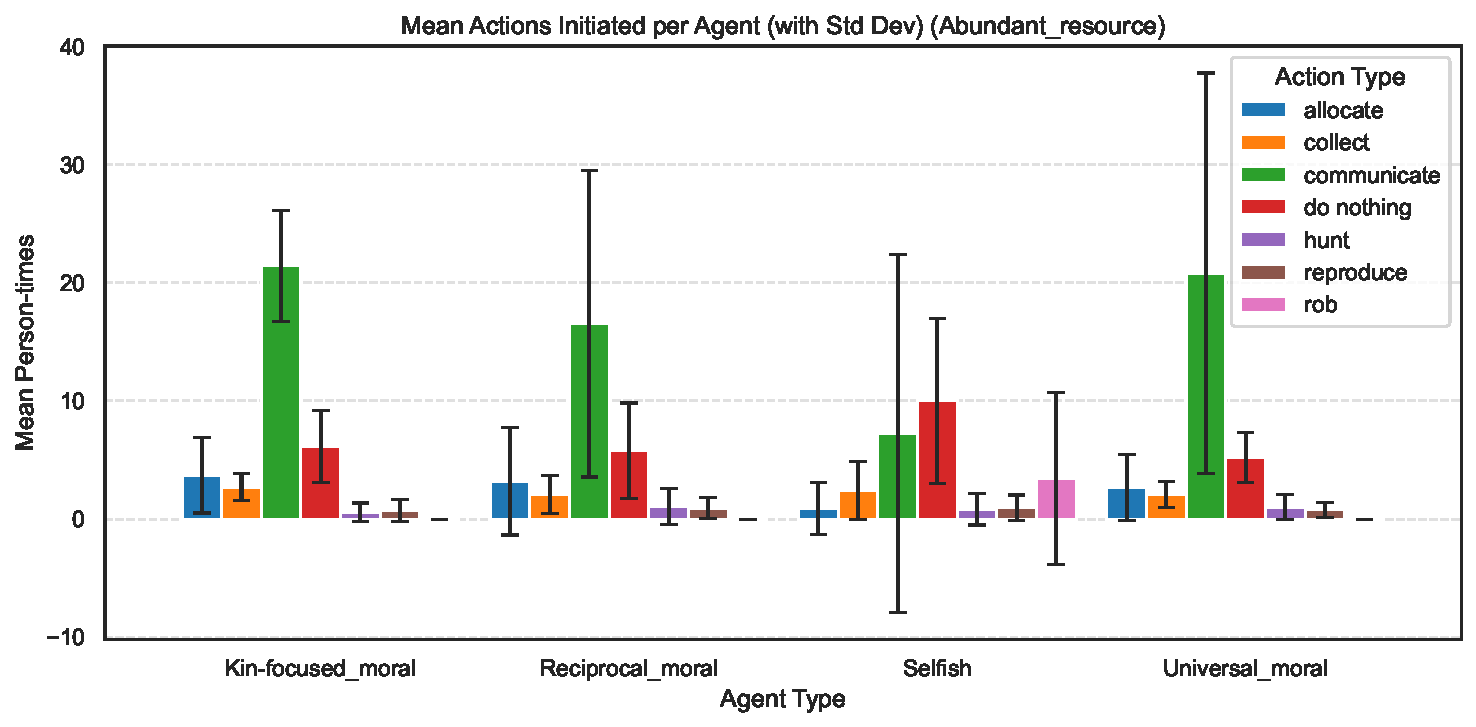
\includegraphics[width=\linewidth]{appendix_figures/actions/action_distri_initiator_by_type_Abundant_resource.pdf}
        \caption{Mean Actions Initiated per Agent}
    \end{subfigure}
    \hfill
    \begin{subfigure}[t]{0.48\textwidth}
        \centering
        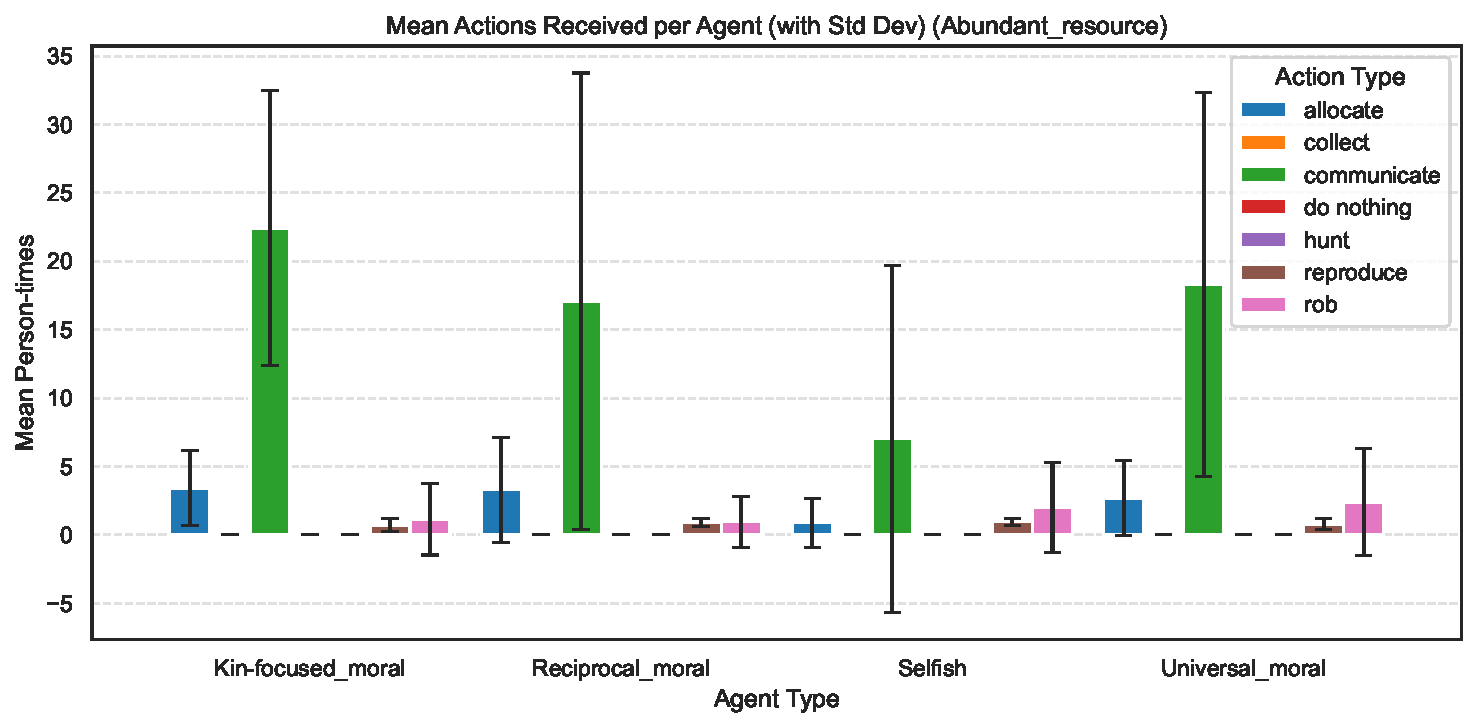
\includegraphics[width=\linewidth]{appendix_figures/actions/action_distri_receiver_by_type_Abundant_resource.pdf}
        \caption{Mean Actions Received per Agent}
    \end{subfigure}
    \caption{Agent-times of action type when agents are initiators and receivers (Case: abundant resource)}
    \label{fig: actions_type_abundant}
\end{figure}

\begin{figure}[H]
    \centering
    \begin{subfigure}[t]{0.48\textwidth}
        \centering
        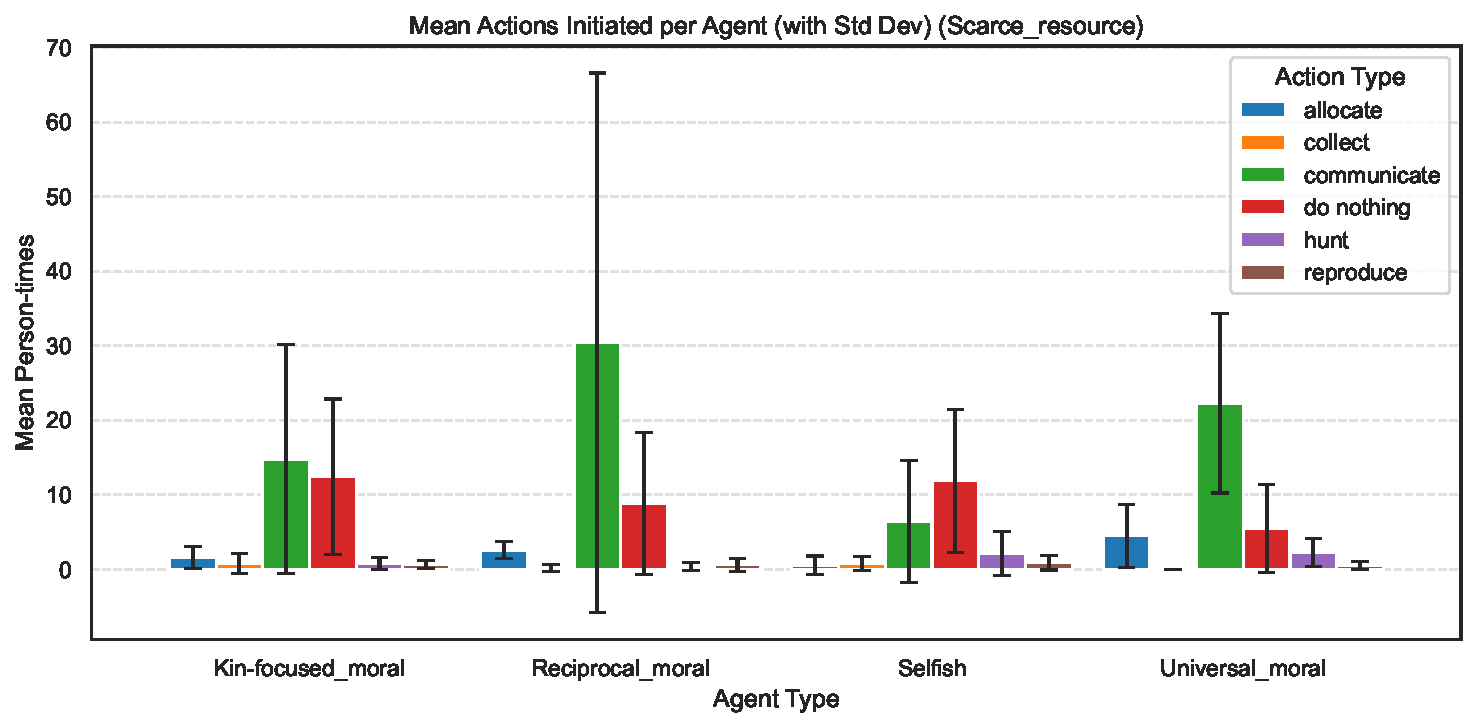
\includegraphics[width=\linewidth]{appendix_figures/actions/action_distri_initiator_by_type_Scarce_resource.pdf}
        \caption{Mean Actions Initiated per Agent}
    \end{subfigure}
    \hfill
    \begin{subfigure}[t]{0.48\textwidth}
        \centering
        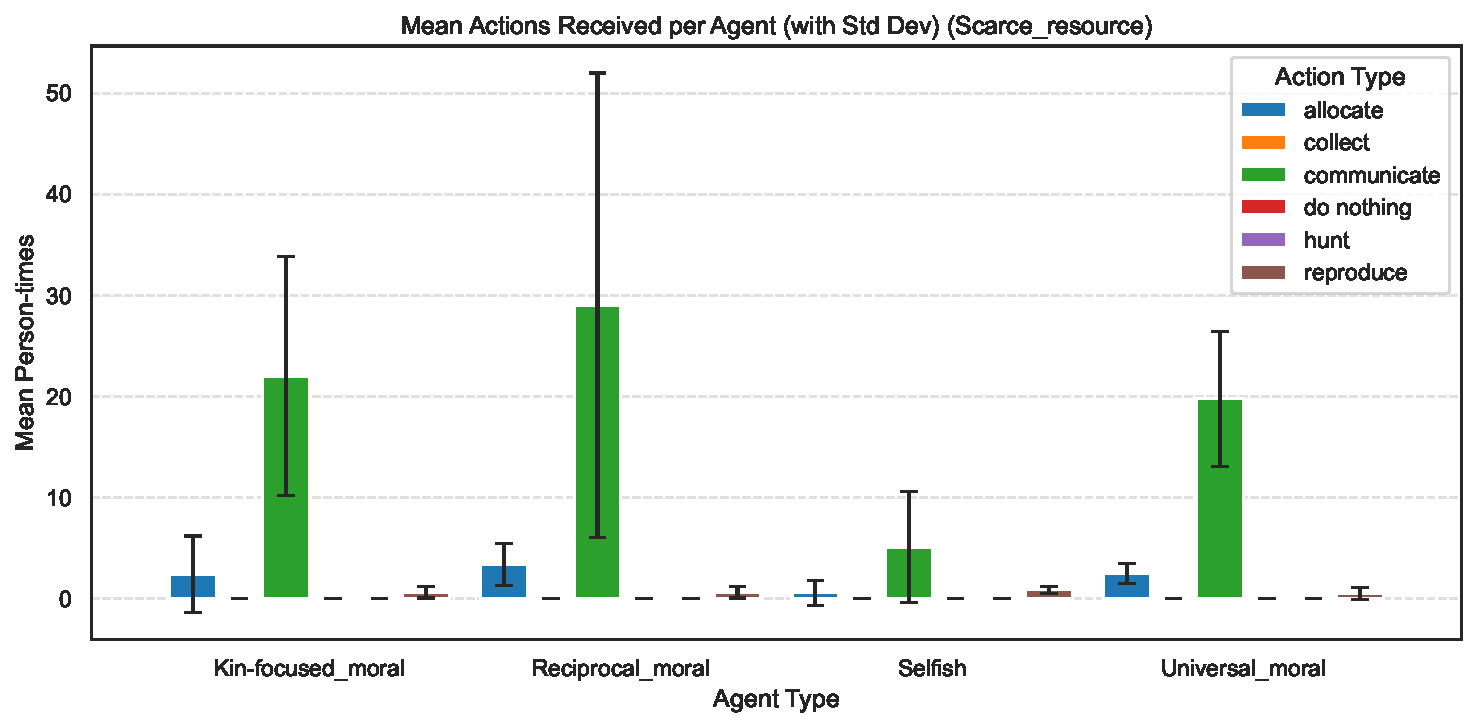
\includegraphics[width=\linewidth]{appendix_figures/actions/action_distri_receiver_by_type_Scarce_resource.pdf}
        \caption{Mean Actions Received per Agent}
    \end{subfigure}
    \caption{Agent-times of action type when agents are initiators and receivers (Case: scarce resource)}
    \label{fig: actions_type_scarce}
\end{figure}

\begin{figure}[H]
    \centering
    \begin{subfigure}[t]{0.48\textwidth}
        \centering
        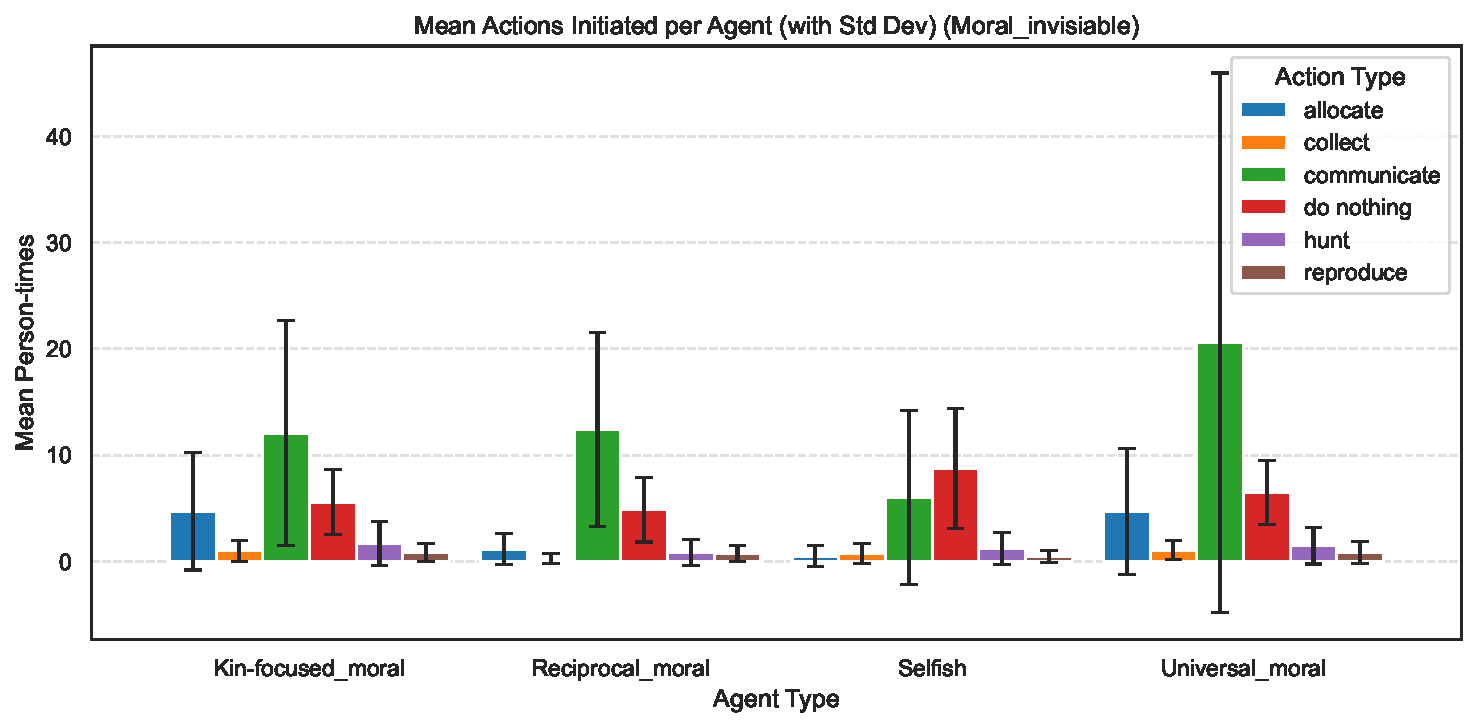
\includegraphics[width=\linewidth]{appendix_figures/actions/action_distri_initiator_by_type_Moral_invisiable.pdf}
        \caption{Mean Actions Initiated per Agent}
    \end{subfigure}
    \hfill
    \begin{subfigure}[t]{0.48\textwidth}
        \centering
        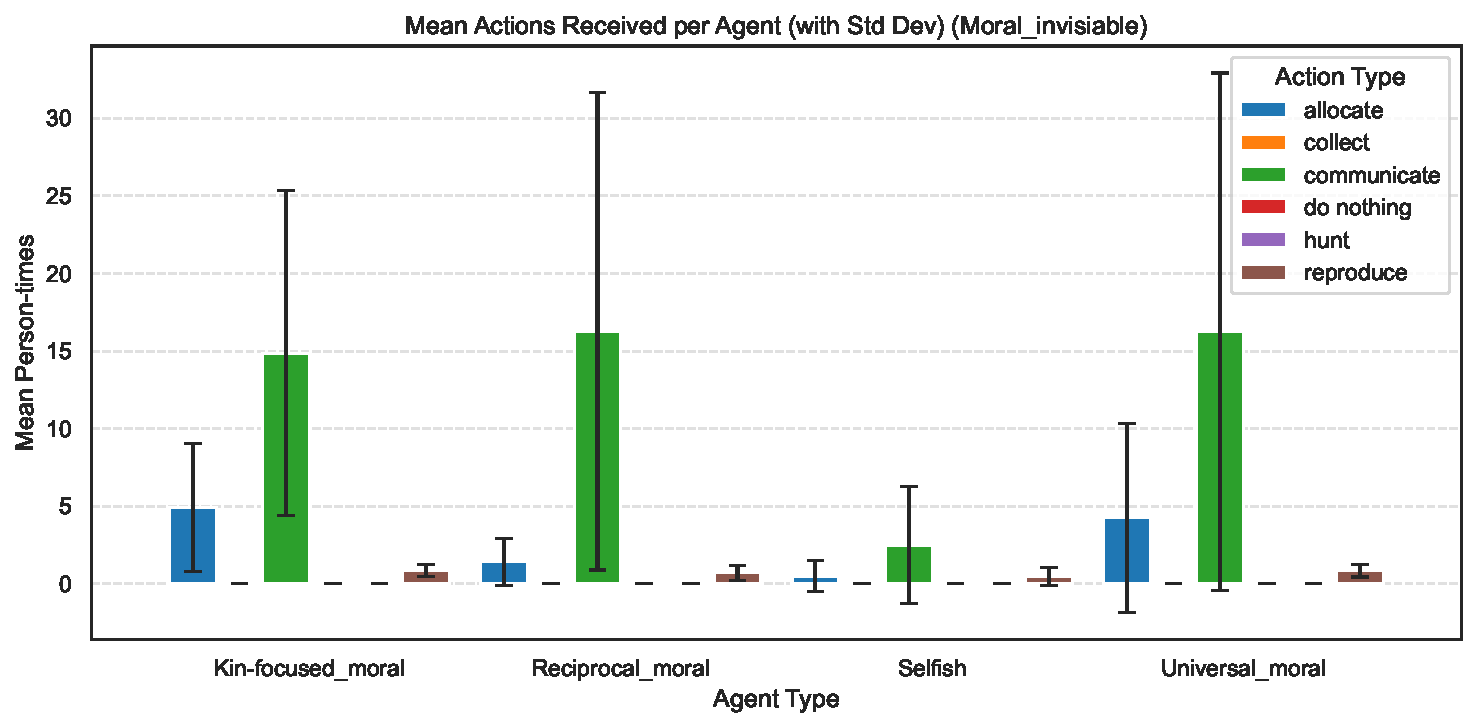
\includegraphics[width=\linewidth]{appendix_figures/actions/action_distri_receiver_by_type_Moral_invisiable.pdf}
        \caption{Mean Actions Received per Agent}
    \end{subfigure}
    \caption{Agent-times of action type when agents are initiators and receivers (Case: moral invisible)}
    \label{fig: actions_type_invisible}
\end{figure}

\begin{figure}[H]
    \centering
    \begin{subfigure}[t]{0.48\textwidth}
        \centering
        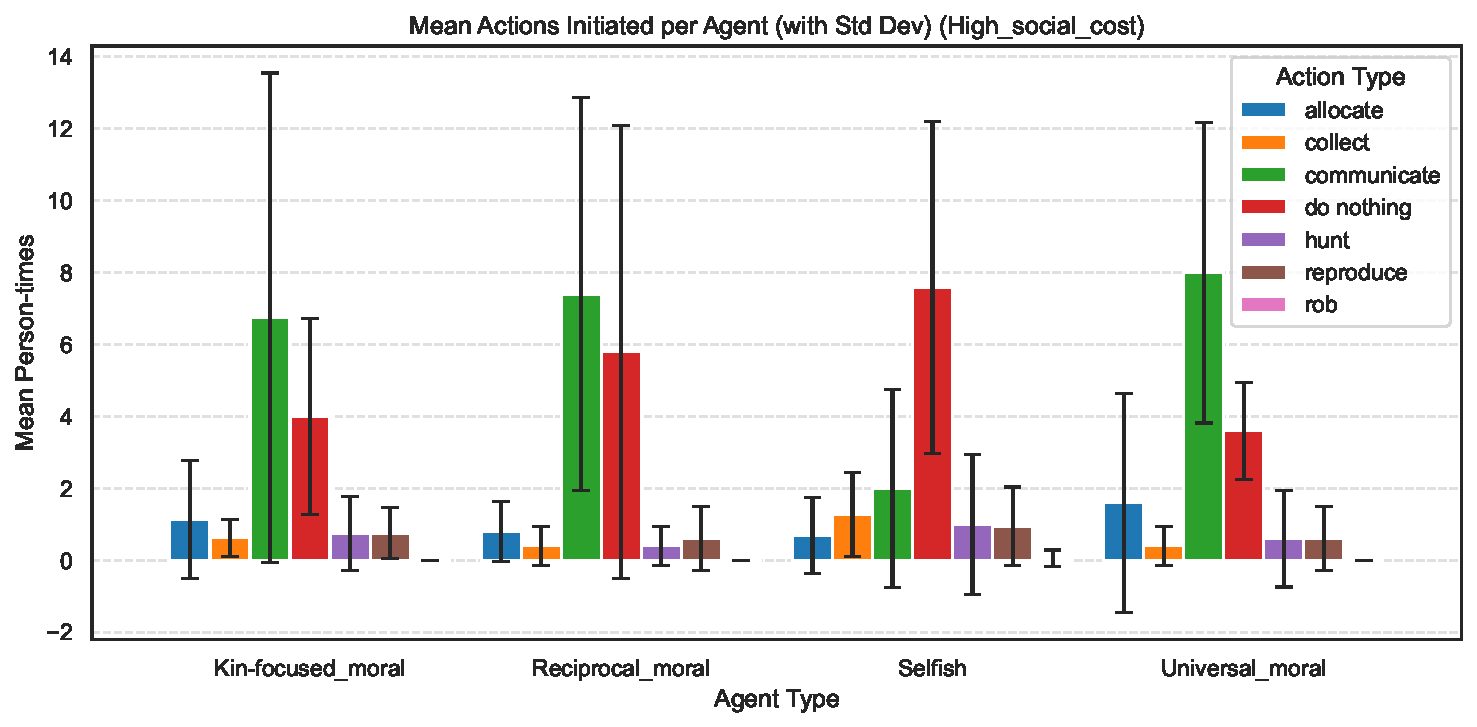
\includegraphics[width=\linewidth]{appendix_figures/actions/action_distri_initiator_by_type_High_social_cost.pdf}
        \caption{Mean Actions Initiated per Agent}
    \end{subfigure}
    \hfill
    \begin{subfigure}[t]{0.48\textwidth}
        \centering
        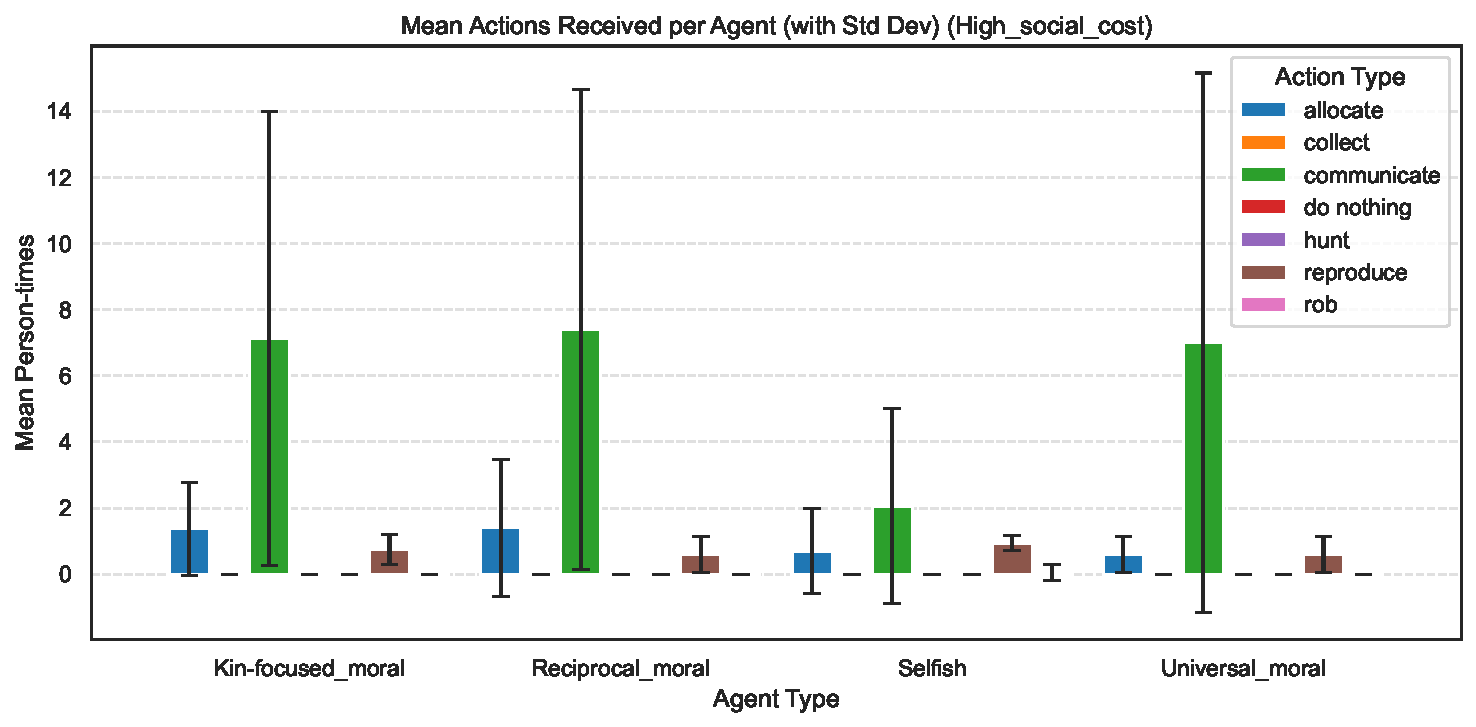
\includegraphics[width=\linewidth]{appendix_figures/actions/action_distri_receiver_by_type_High_social_cost.pdf}
        \caption{Mean Actions Received per Agent}
    \end{subfigure}
    \caption{Agent-times of action type when agents are initiators and receivers (Case: high social cost)}
    \label{fig: actions_type_social_cost}
\end{figure}

\begin{figure}[H]
    \centering
    \begin{subfigure}[t]{0.48\textwidth}
        \centering
        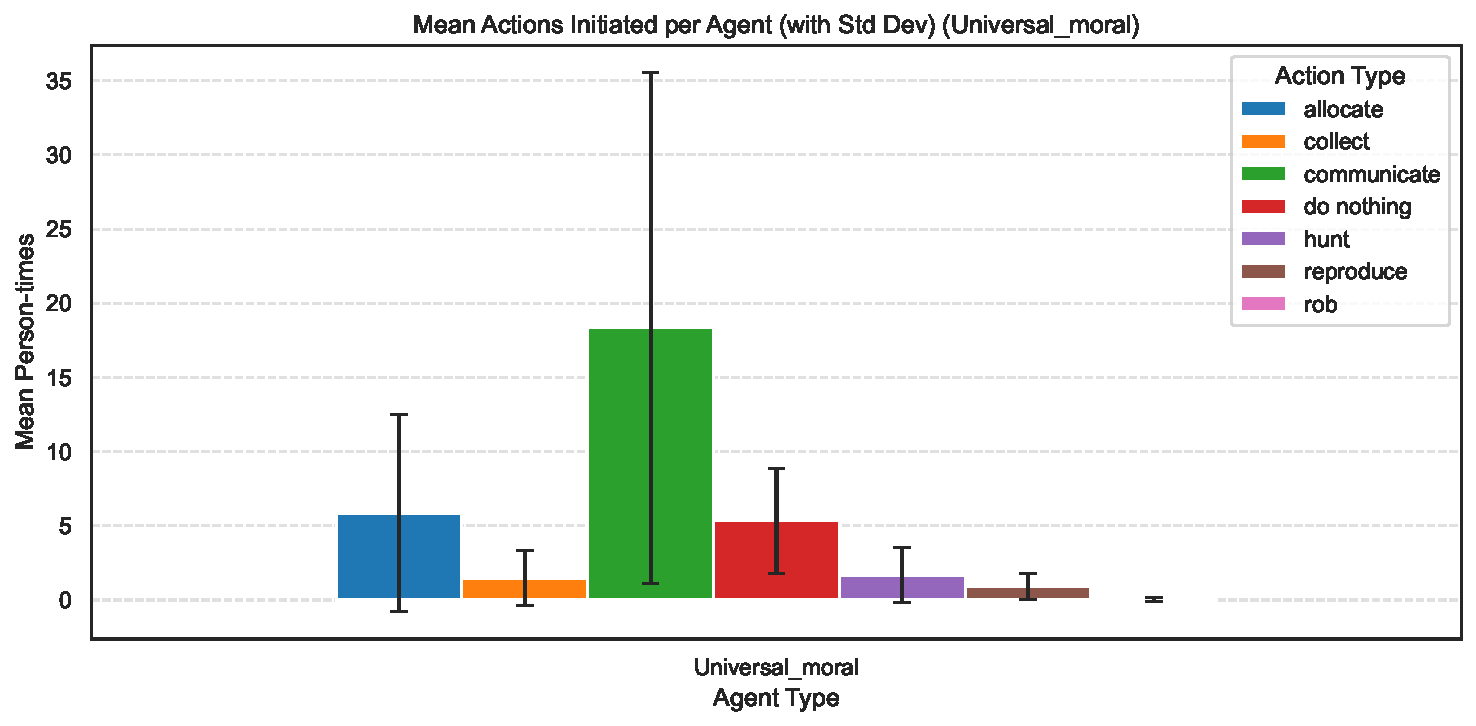
\includegraphics[width=\linewidth]{appendix_figures/actions/action_distri_initiator_by_type_Universal_moral.pdf}
        \caption{Mean Actions Initiated per Agent}
    \end{subfigure}
    \hfill
    \begin{subfigure}[t]{0.48\textwidth}
        \centering
        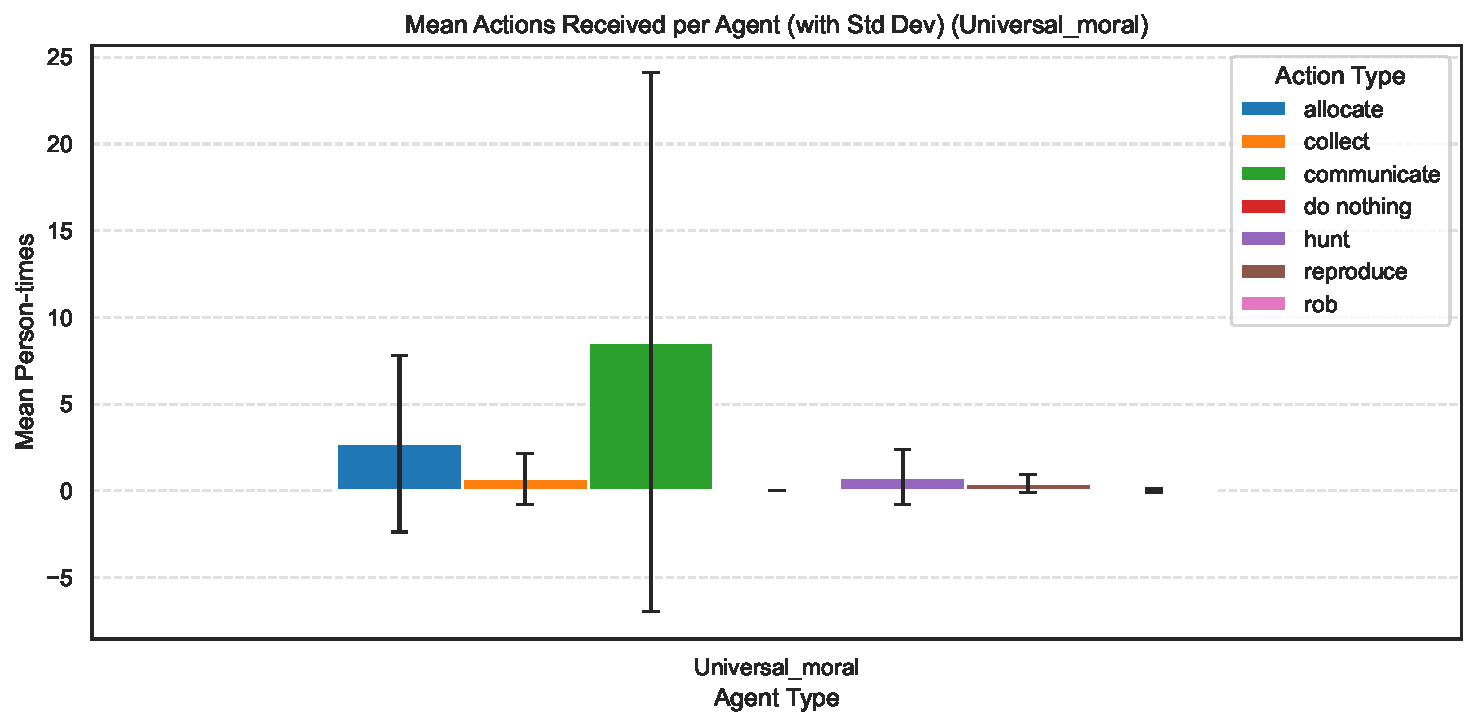
\includegraphics[width=\linewidth]{appendix_figures/actions/action_distri_receiver_by_type_Universal_moral.pdf}
        \caption{Mean Actions Received per Agent}
    \end{subfigure}
    \caption{Agent-times of action type when agents are initiators and receivers (Case: universal)}
    \label{fig: actions_type_universal}
\end{figure}

\begin{figure}[H]
    \centering
    \begin{subfigure}[t]{0.48\textwidth}
        \centering
        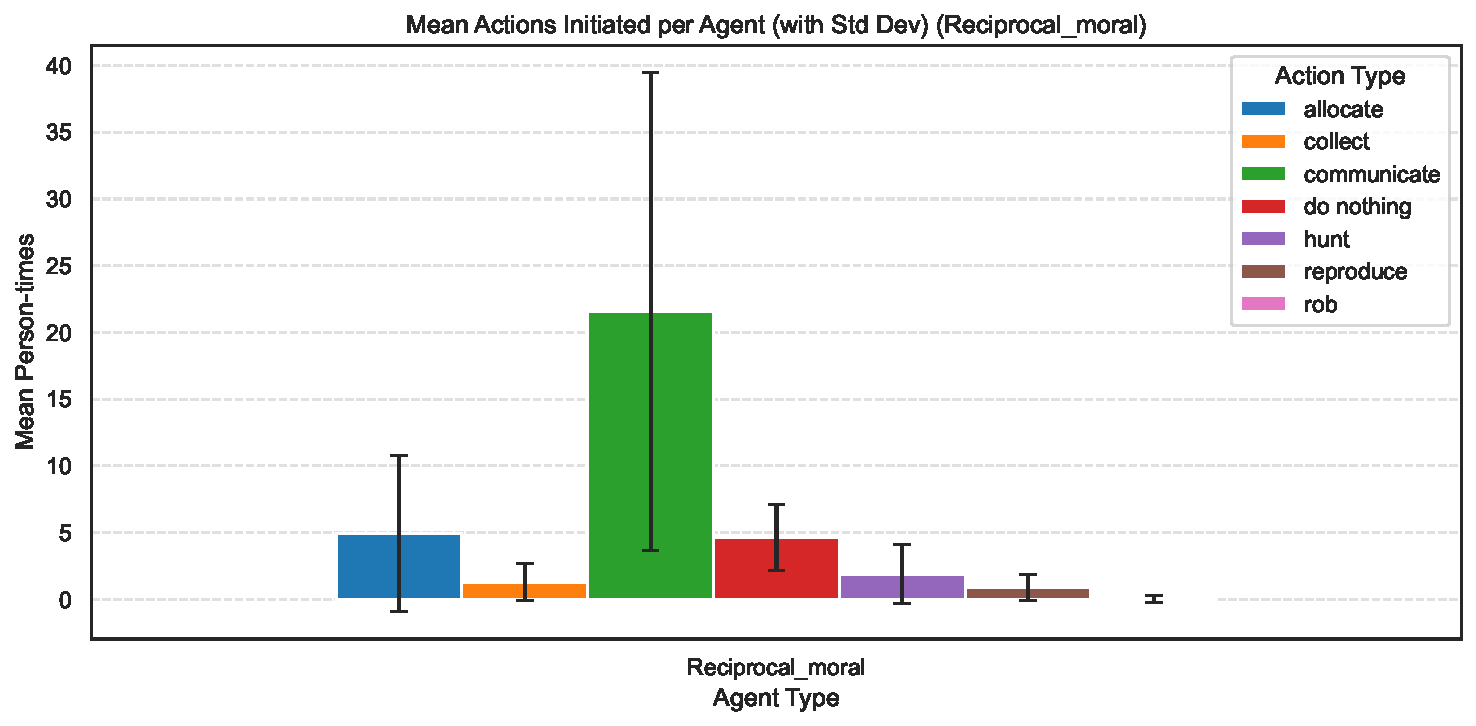
\includegraphics[width=\linewidth]{appendix_figures/actions/action_distri_initiator_by_type_Reciprocal_moral.pdf}
        \caption{Mean Actions Initiated per Agent}
    \end{subfigure}
    \hfill
    \begin{subfigure}[t]{0.48\textwidth}
        \centering
        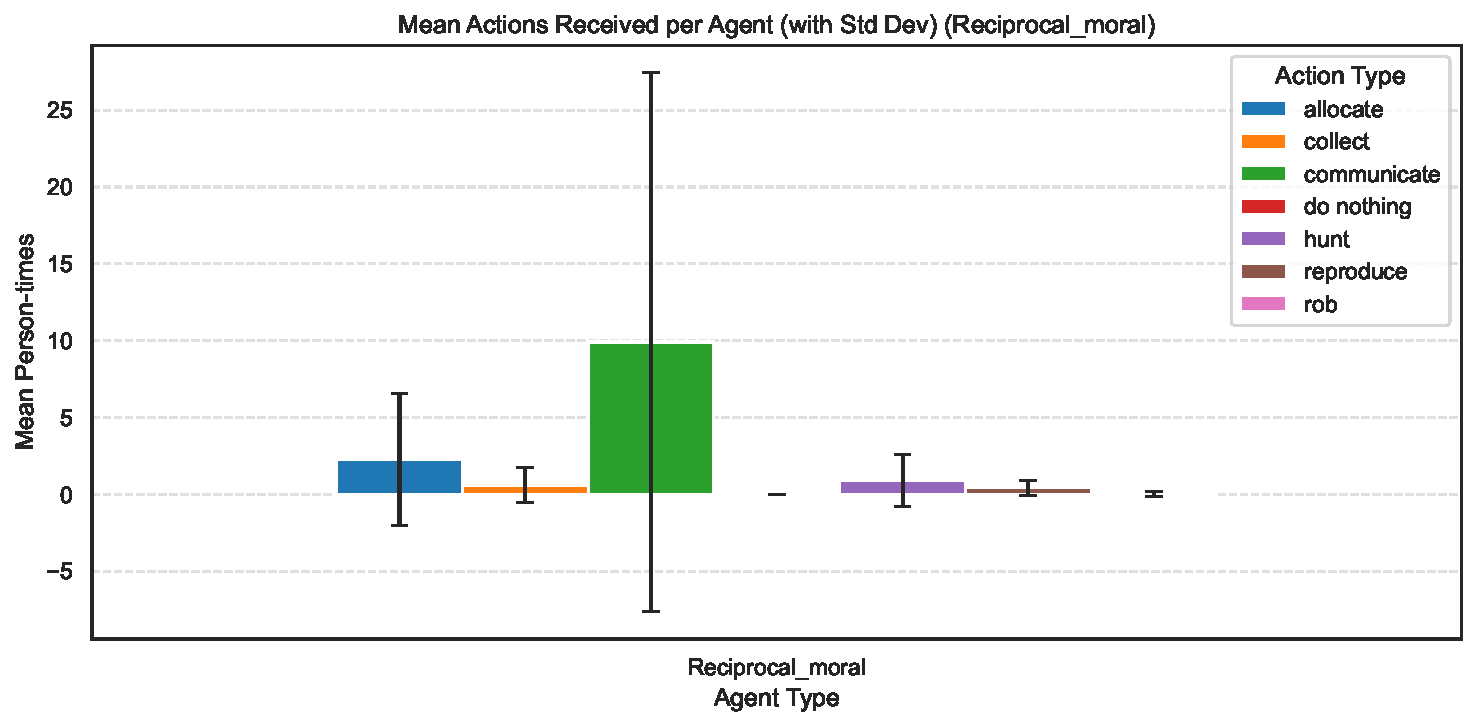
\includegraphics[width=\linewidth]{appendix_figures/actions/action_distri_receiver_by_type_Reciprocal_moral.pdf}
        \caption{Mean Actions Received per Agent}
    \end{subfigure}
    \caption{Agent-times of action type when agents are initiators and receivers (Case: reciprocal)}
    \label{fig: actions_type_reciprocal}
\end{figure}

\begin{figure}[H]
    \centering
    \begin{subfigure}[t]{0.48\textwidth}
        \centering
        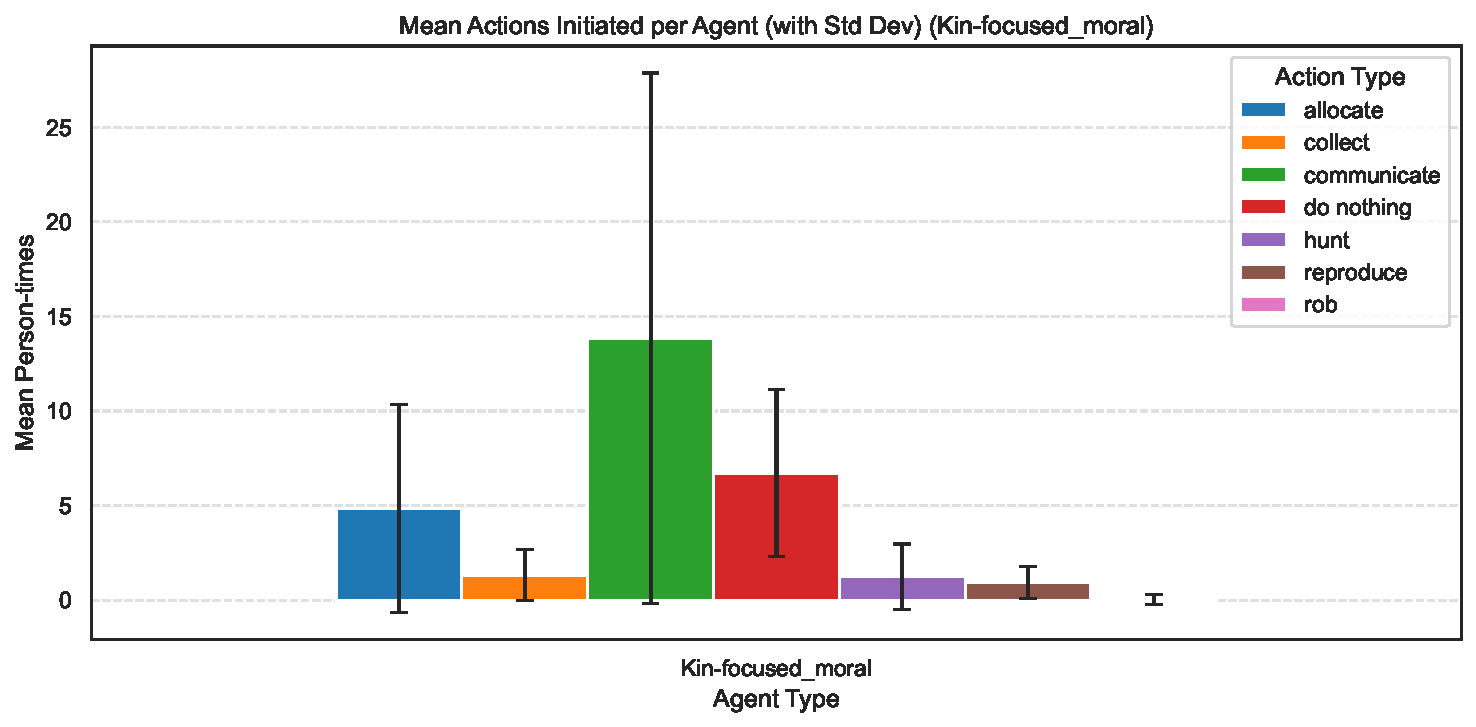
\includegraphics[width=\linewidth]{appendix_figures/actions/action_distri_initiator_by_type_Kin-focused_moral.pdf}
        \caption{Mean Actions Initiated per Agent}
    \end{subfigure}
    \hfill
    \begin{subfigure}[t]{0.48\textwidth}
        \centering
        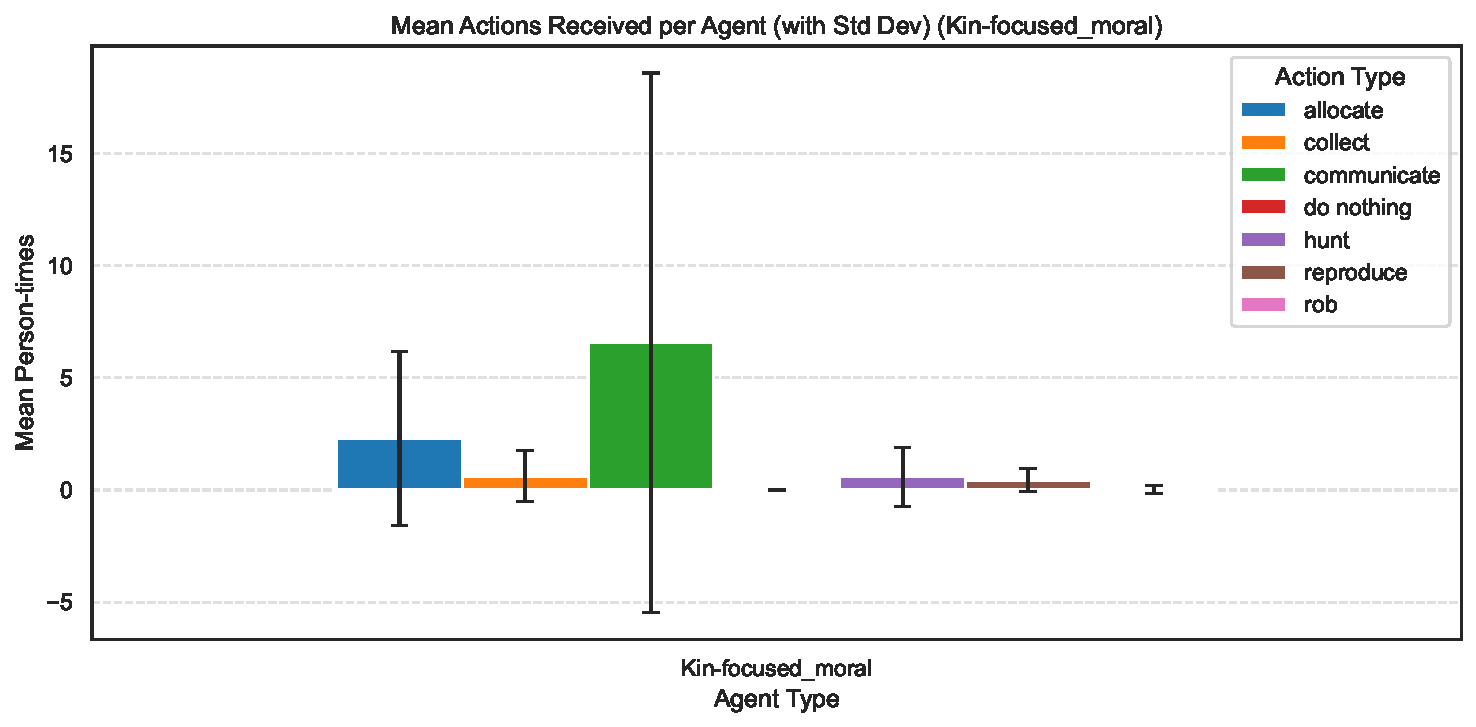
\includegraphics[width=\linewidth]{appendix_figures/actions/action_distri_receiver_by_type_Kin-focused_moral.pdf}
        \caption{Mean Actions Received per Agent}
    \end{subfigure}
    \caption{Agent-times of action type when agents are initiators and receivers (Case: kin)}
    \label{fig: actions_type_kin}
\end{figure}

\begin{figure}[H]
    \centering
    \begin{subfigure}[t]{0.48\textwidth}
        \centering
        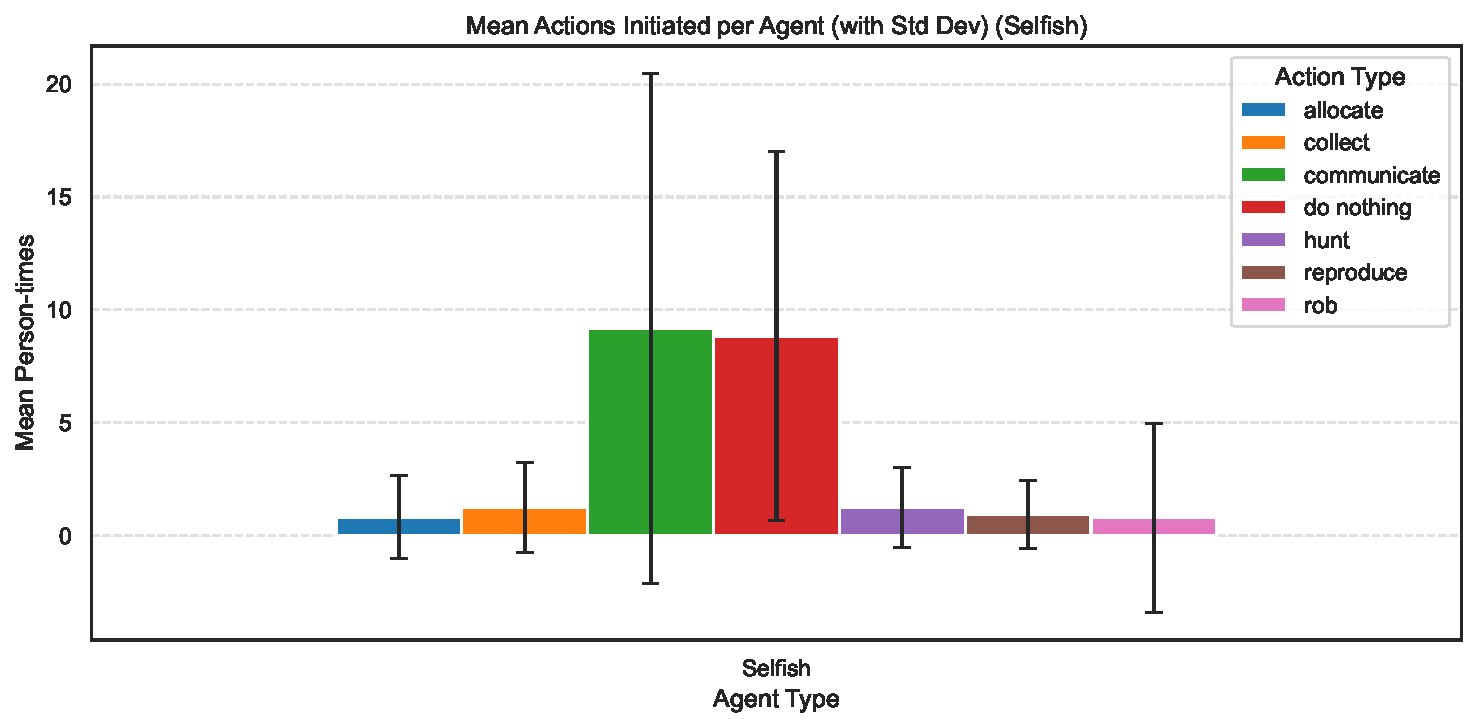
\includegraphics[width=\linewidth]{appendix_figures/actions/action_distri_initiator_by_type_Selfish.pdf}
        \caption{Mean Actions Initiated per Agent}
    \end{subfigure}
    \hfill
    \begin{subfigure}[t]{0.48\textwidth}
        \centering
        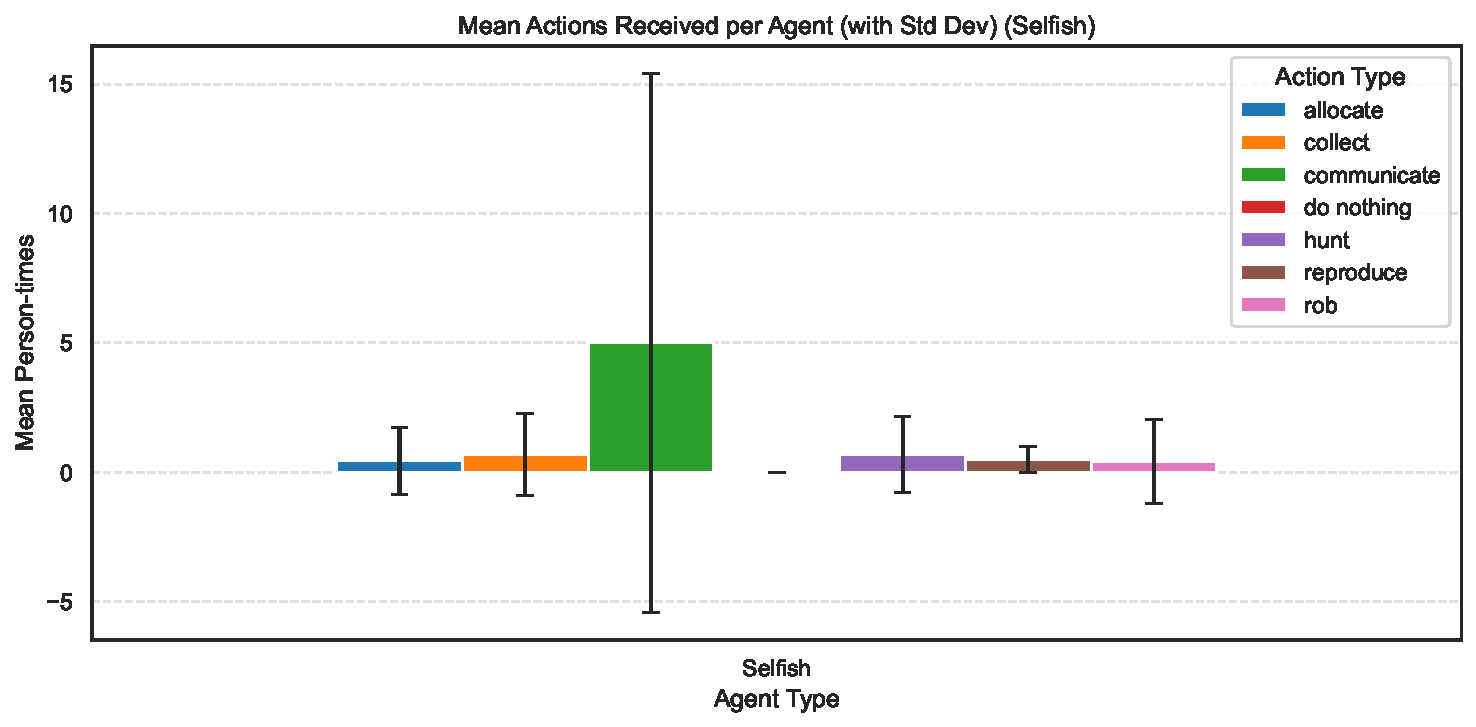
\includegraphics[width=\linewidth]{appendix_figures/actions/action_distri_receiver_by_type_Selfish.pdf}
        \caption{Mean Actions Received per Agent}
    \end{subfigure}
    \caption{Agent-times of action type when agents are initiators and receivers (Case: selfish)}
    \label{fig: actions_type_selfish}
\end{figure}


\subsubsection{HP gain and loss of each action type}

Figures~\ref{fig: HP_action_resource} to \ref{fig: HP_action_single} explore the health point (HP) gain and loss associated with different action types. Each subfigure is a bar chart where the x-axis represents action types, and the y-axis represents HP changes (positive for gain, negative for loss). Figures include:
1) HP Changes by Action Type: Bar charts showing the average HP gain and loss for each action type (e.g., hunting, resting, social interactions). The x-axis represents action types, and the y-axis represents HP changes.
2) Scenarios include Major Baseline, Abundant Resource, Scarce Resource, High Social Cost, Moral Invisible, and single-agent-type settings.

From all these figures, we could conclude that:
\begin{itemize}
    \item Collect and hunt are the main sources of HP for all types of agents
    \item Universal moral and kin-focused moral agent gains lots of allocation
    \item Robbery is also a source of HP for selfish agents.
\end{itemize}

\begin{figure}[H]
    \centering

    % 第一行
    \begin{subfigure}[t]{0.48\textwidth}
        \centering
        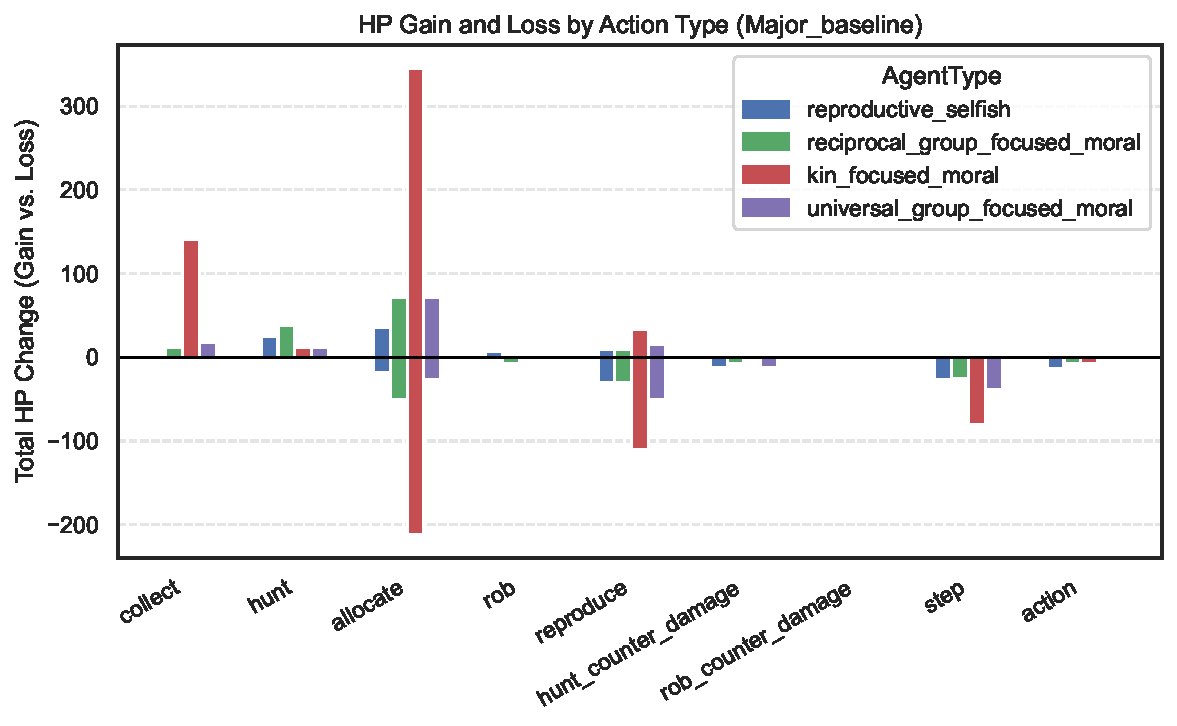
\includegraphics[width=\linewidth]{appendix_figures/HP/hp_change_by_action_Major_baseline.pdf}
        \caption{HP Gain and Loss by Action Type (Case: major baseline)}
    \end{subfigure}
    \hfill
    \begin{subfigure}[t]{0.48\textwidth}
        \centering
        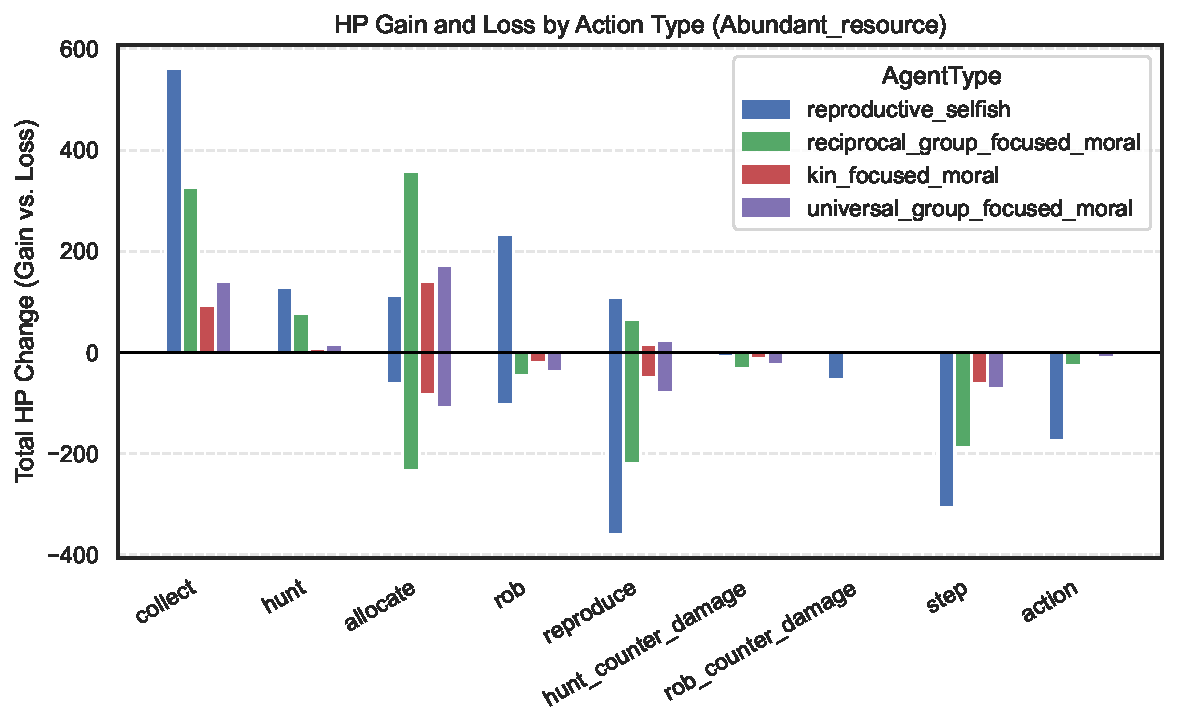
\includegraphics[width=\linewidth]{appendix_figures/HP/hp_change_by_action_Abundant_resource.pdf}
        \caption{HP Gain and Loss by Action Type (Case: abundant resource)}
    \end{subfigure}
    \hfill
    
    \begin{subfigure}[t]{0.48\textwidth}
        \centering
        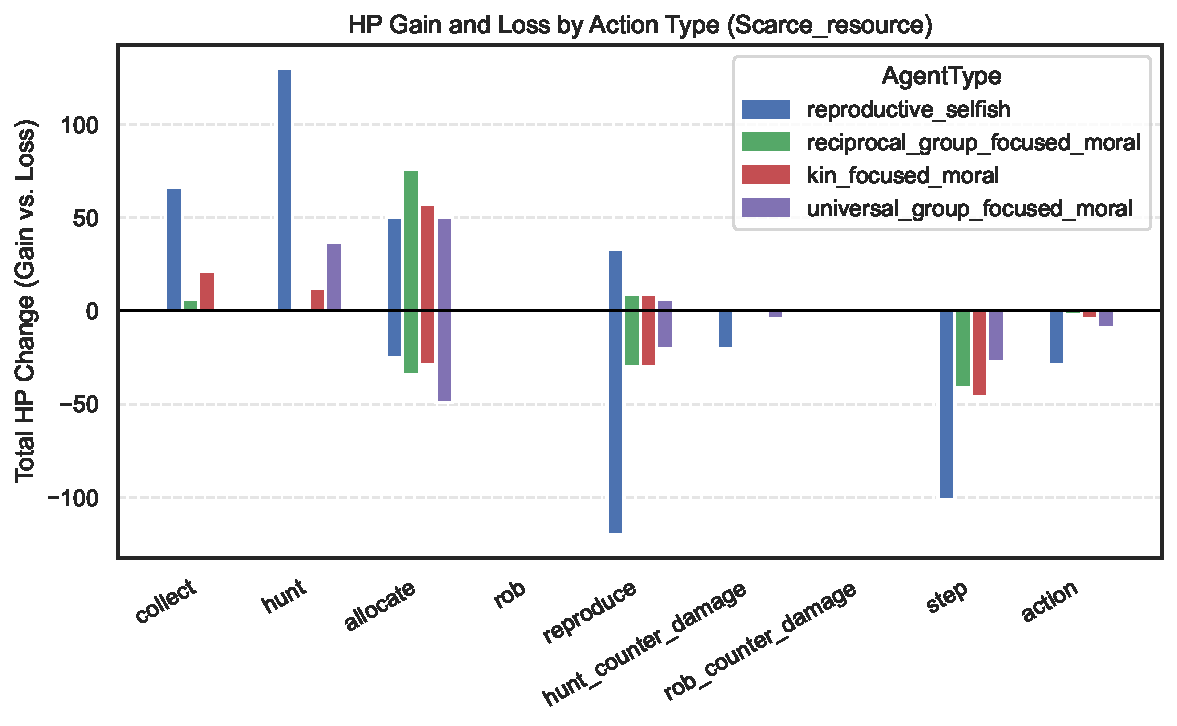
\includegraphics[width=\linewidth]{appendix_figures/HP/hp_change_by_action_Scarce_resource.pdf}
        \caption{HP Gain and Loss by Action Type (Case: scarce resource)}
    \end{subfigure}
    \hfill
    \caption{HP Gain and Loss by Action Type (Cases: major baseline, abundant resource, and scarce resource)}
    \label{fig: HP_action_resource}
\end{figure}

\begin{figure}[H]
    \centering
    \begin{subfigure}[t]{0.48\textwidth}
        \centering
        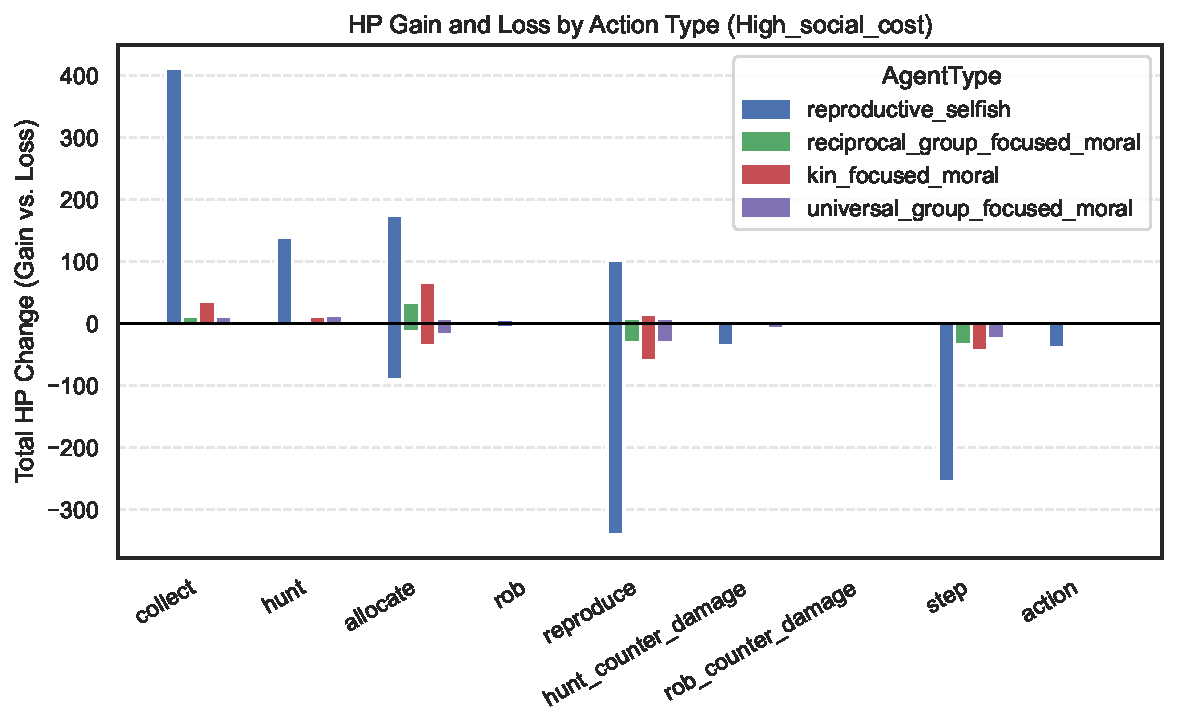
\includegraphics[width=\linewidth]{appendix_figures/HP/hp_change_by_action_High_social_cost.pdf}
        \caption{HP Gain and Loss by Action Type (Case: high social cost)}
    \end{subfigure}
    \hfill
    \begin{subfigure}[t]{0.48\textwidth}
        \centering
        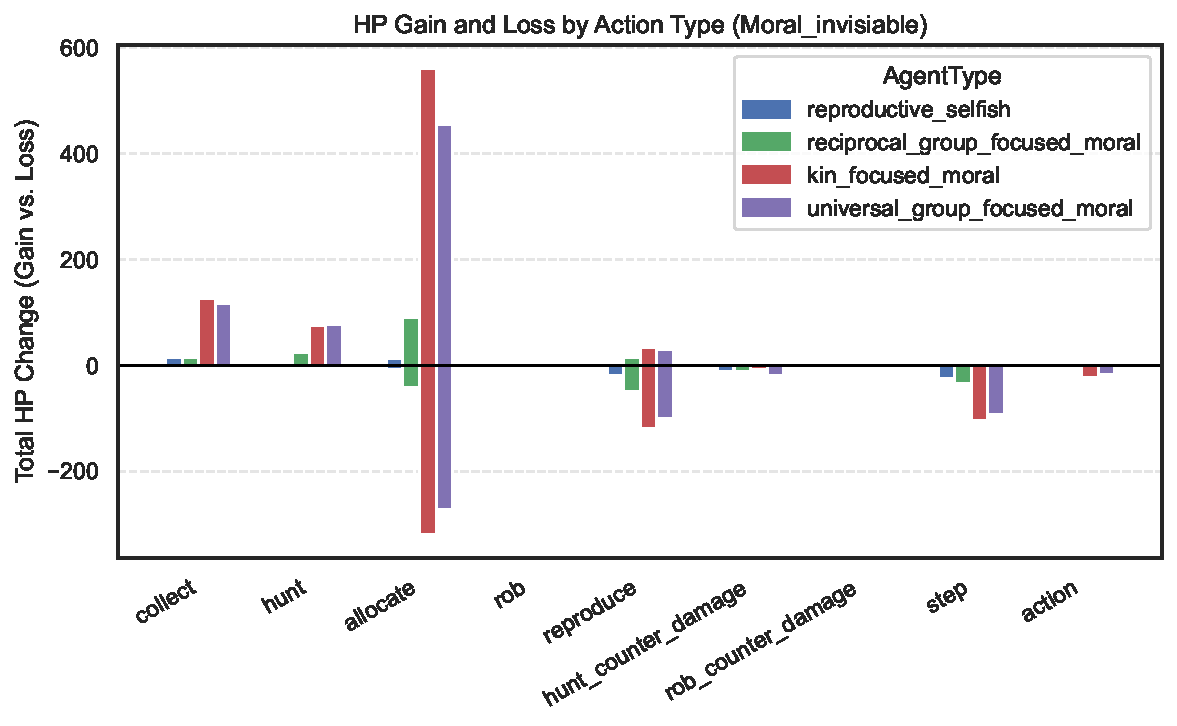
\includegraphics[width=\linewidth]{appendix_figures/HP/hp_change_by_action_Moral_invisiable.pdf}
        \caption{HP Gain and Loss by Action Type (Case: moral invisible)}
    \end{subfigure}
    \hfill

    \caption{HP Gain and Loss by Action Type (Cases: high social cost and moral invisible)}
    \label{fig: HP_action_invisible}
\end{figure}

\begin{figure}[H]
    \centering
    \begin{subfigure}[t]{0.48\textwidth}
        \centering
        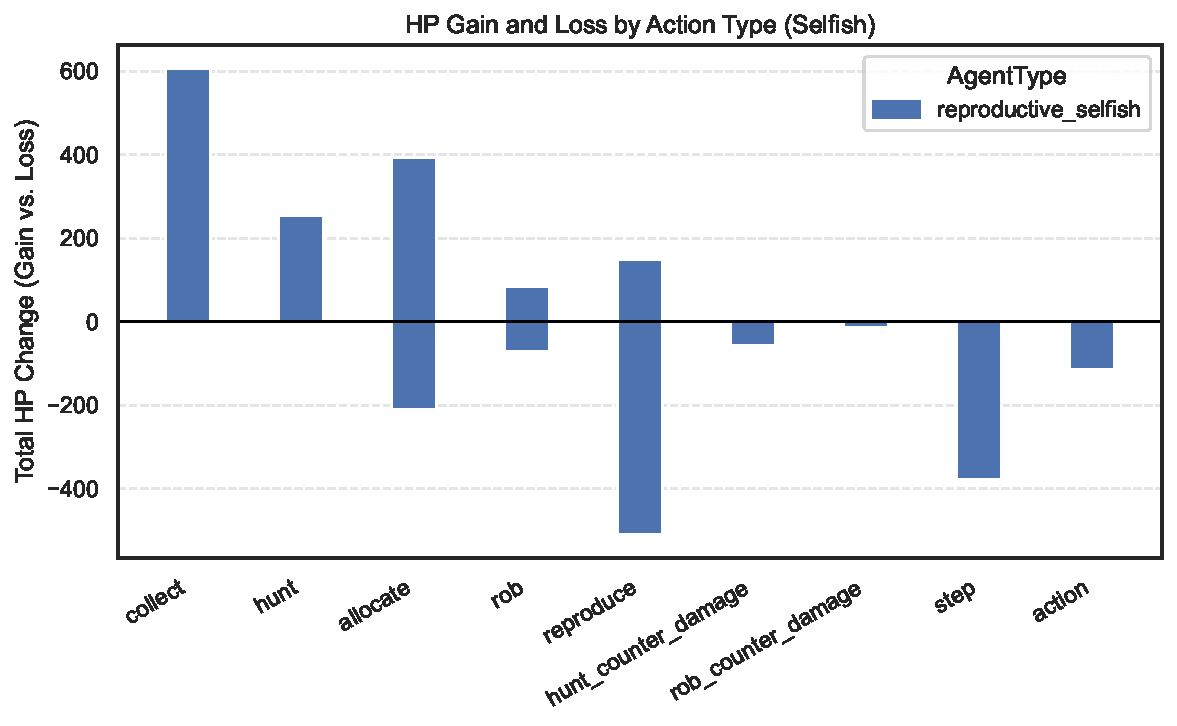
\includegraphics[width=\linewidth]{appendix_figures/HP/hp_change_by_action_Selfish.pdf}
        \caption{HP Gain and Loss by Action Type (Case: selfish)}
    \end{subfigure}
    \hfill
    \begin{subfigure}[t]{0.48\textwidth}
        \centering
        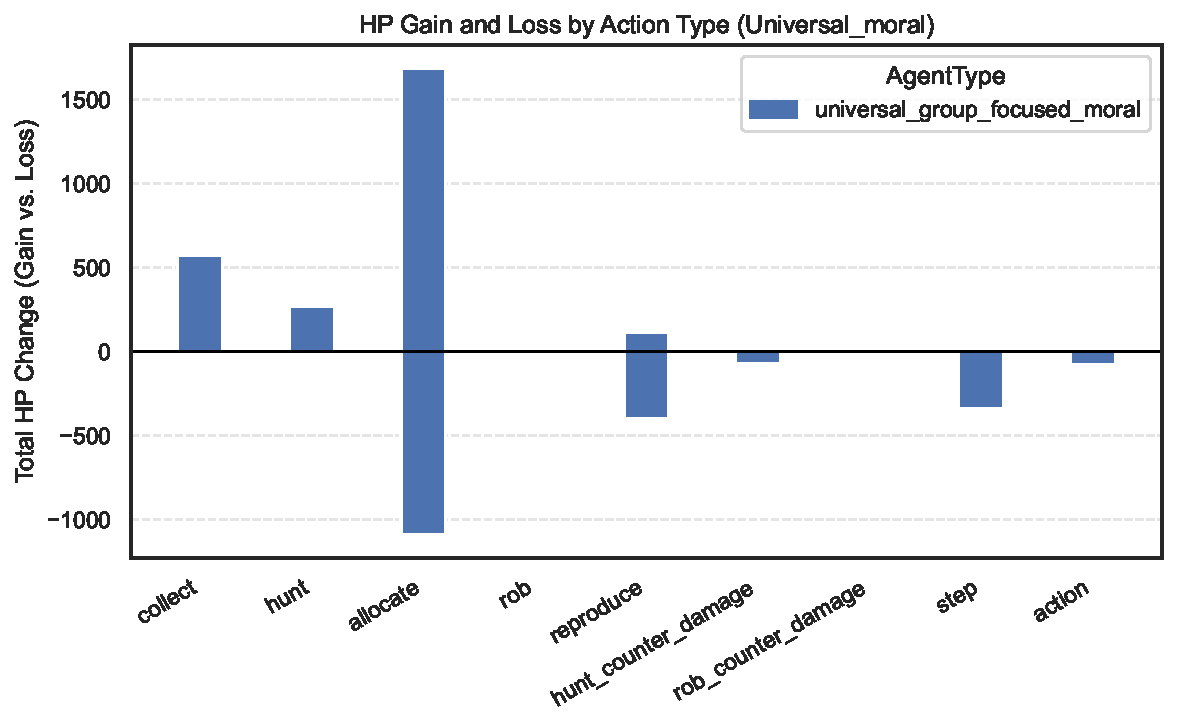
\includegraphics[width=\linewidth]{appendix_figures/HP/hp_change_by_action_Universal_moral.pdf}
        \caption{HP Gain and Loss by Action Type (Case: universal)}
    \end{subfigure}
    \hfill
    
    \begin{subfigure}[t]{0.48\textwidth}
        \centering
        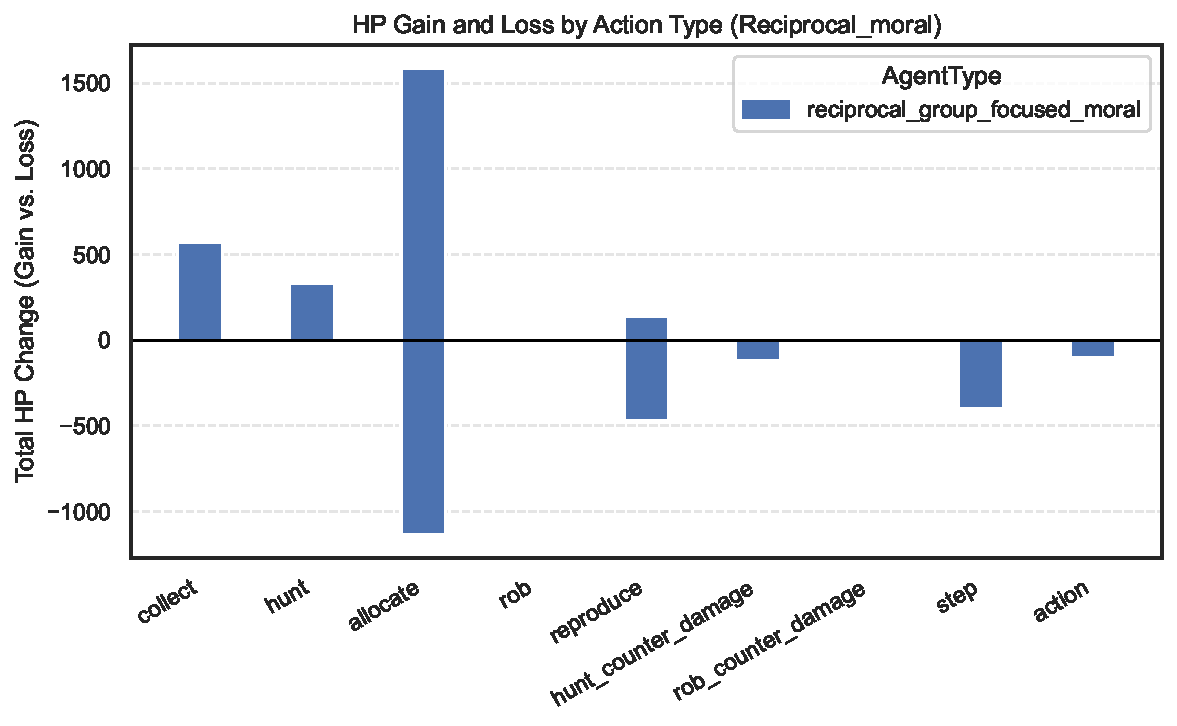
\includegraphics[width=\linewidth]{appendix_figures/HP/hp_change_by_action_Reciprocal_moral.pdf}
        \caption{HP Gain and Loss by Action Type (Case: reciprocal)}
    \end{subfigure}
    \hfill
    \begin{subfigure}[t]{0.48\textwidth}
        \centering
        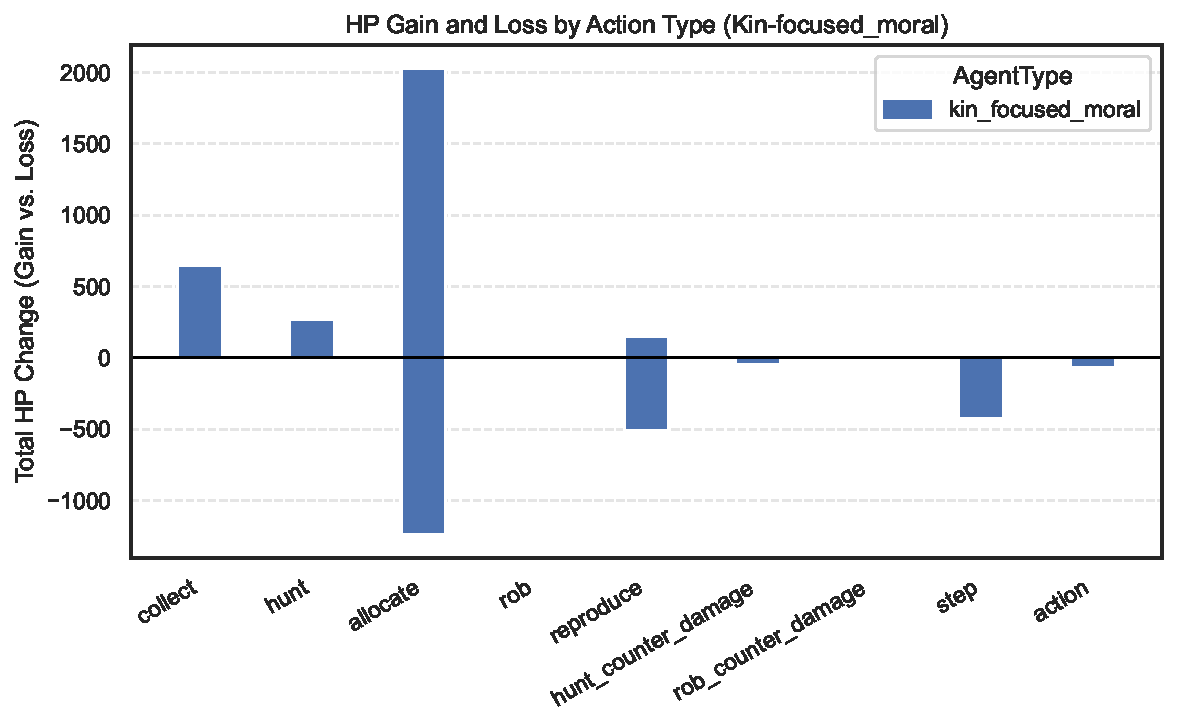
\includegraphics[width=\linewidth]{appendix_figures/HP/hp_change_by_action_Kin-focused_moral.pdf}
        \caption{HP Gain and Loss by Action Type (Case: kin)}
    \end{subfigure}

    \caption{HP Gain and Loss by Action Type with single agent type settings}
    \label{fig: HP_action_single}
\end{figure}


\subsubsection{Family network}

Figures~\ref{fig: family network major} to \ref{fig: family network kin} visualize family lineage networks for agents under different scenarios. Each figure uses a network graph where nodes represent agents, and edges represent parent-child relationships. Node colors and sizes may indicate agent types or lifespan.

From all these figures, we could conclude that:
\begin{itemize}
    \item Agents barely reproduce more than twice, except when resources are abundant
    \item Kin-focused moral agents in general have the most generation
    \item Only one family can survive until the end
\end{itemize}

\begin{figure}[H]
    \centering
        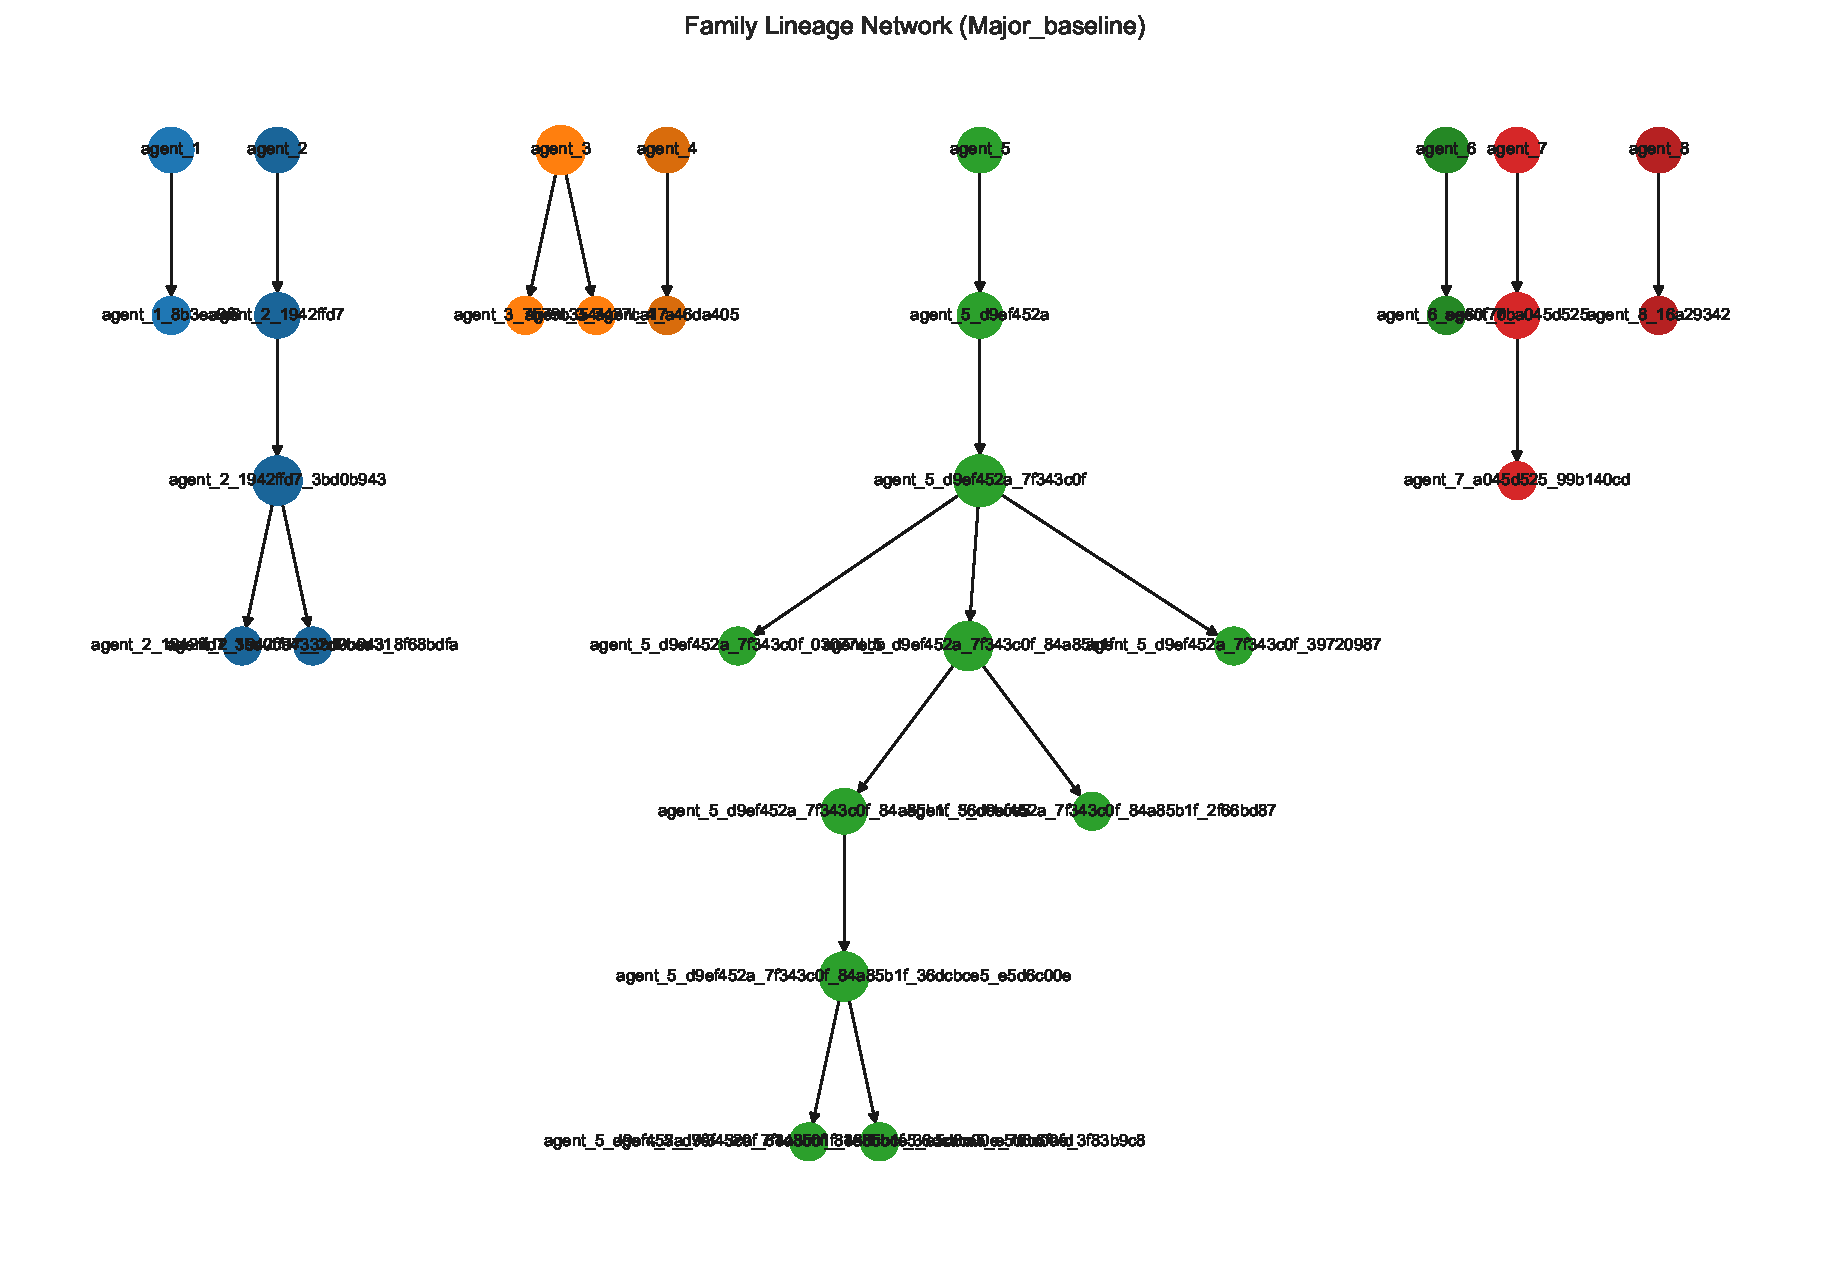
\includegraphics[width=\linewidth]{appendix_figures/networks/family_network_Major_baseline.pdf}
    \caption{Family Lineage Network for Major Baseline}
    \label{fig: family network major}
\end{figure}

\begin{figure}[H]
    \centering
        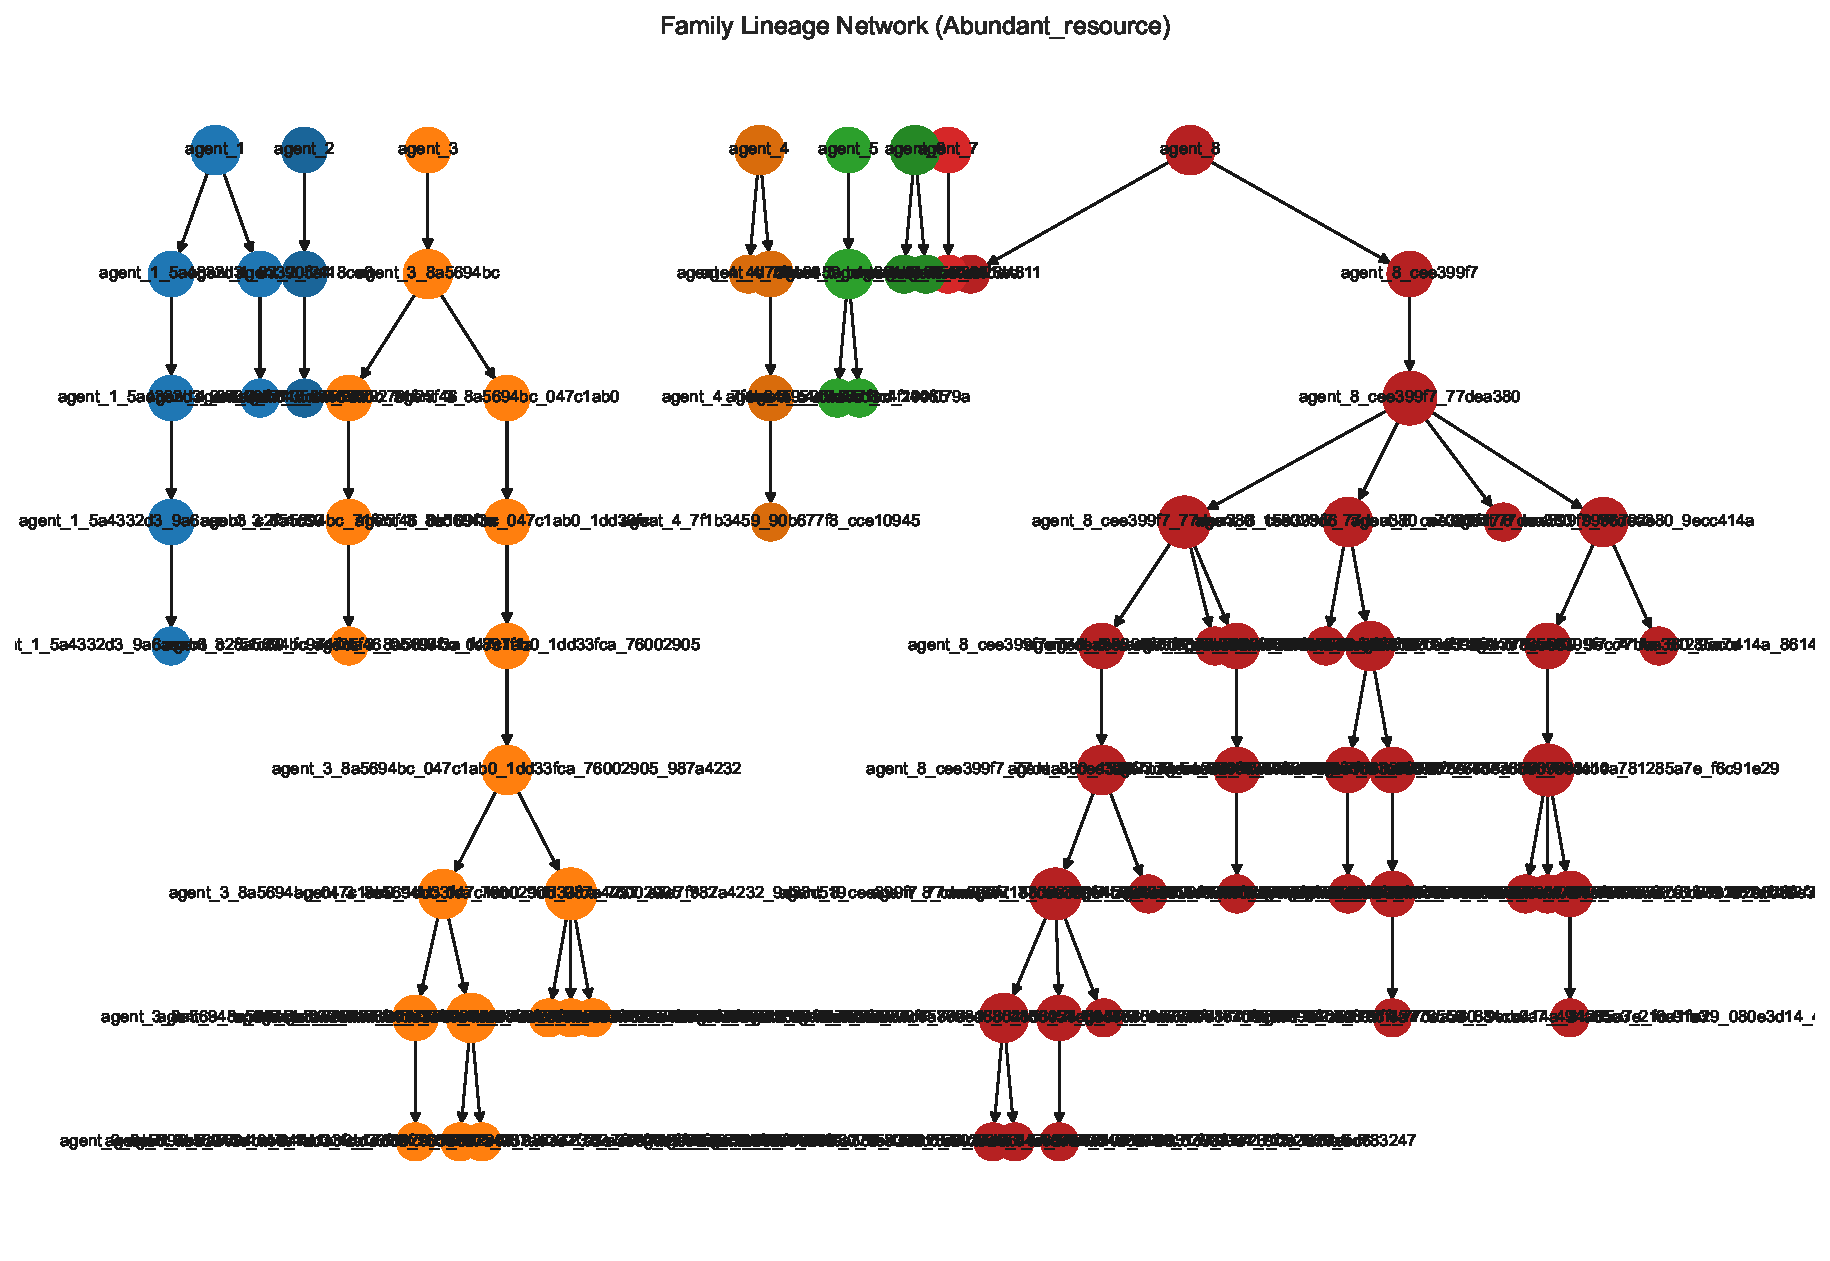
\includegraphics[width=\linewidth]{appendix_figures/networks/family_network_Abundant_resource.pdf}
    \caption{Family Lineage Network for Abundant Resource}
    \label{fig: family network abundant}
\end{figure}
    
\begin{figure}[H]
    \centering   
        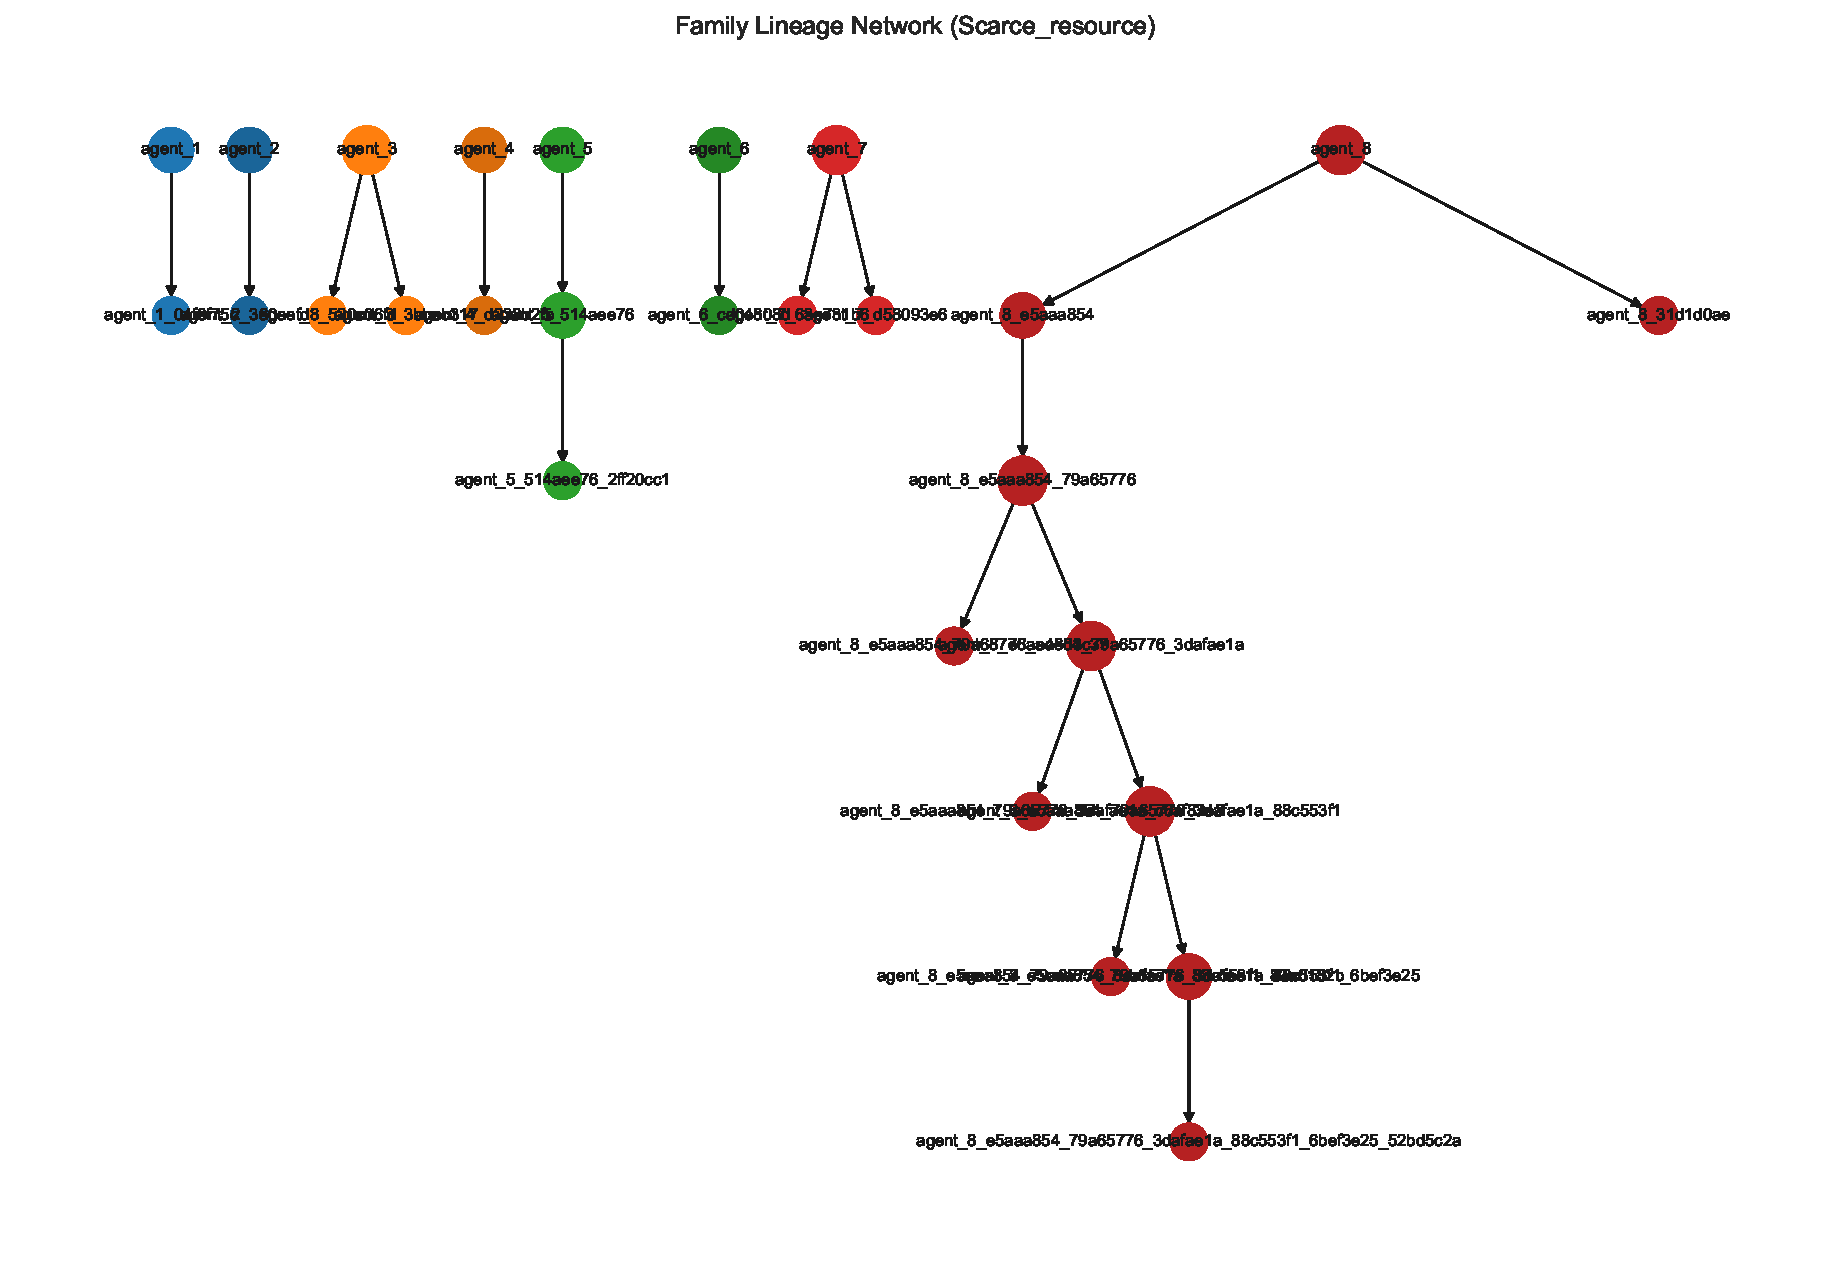
\includegraphics[width=\linewidth]{appendix_figures/networks/family_network_Scarce_resource.pdf}
    \caption{Family Lineage Network for Scarce Resource}
    \label{fig: family network scarce}
\end{figure}

\begin{figure}[H]
    \centering
        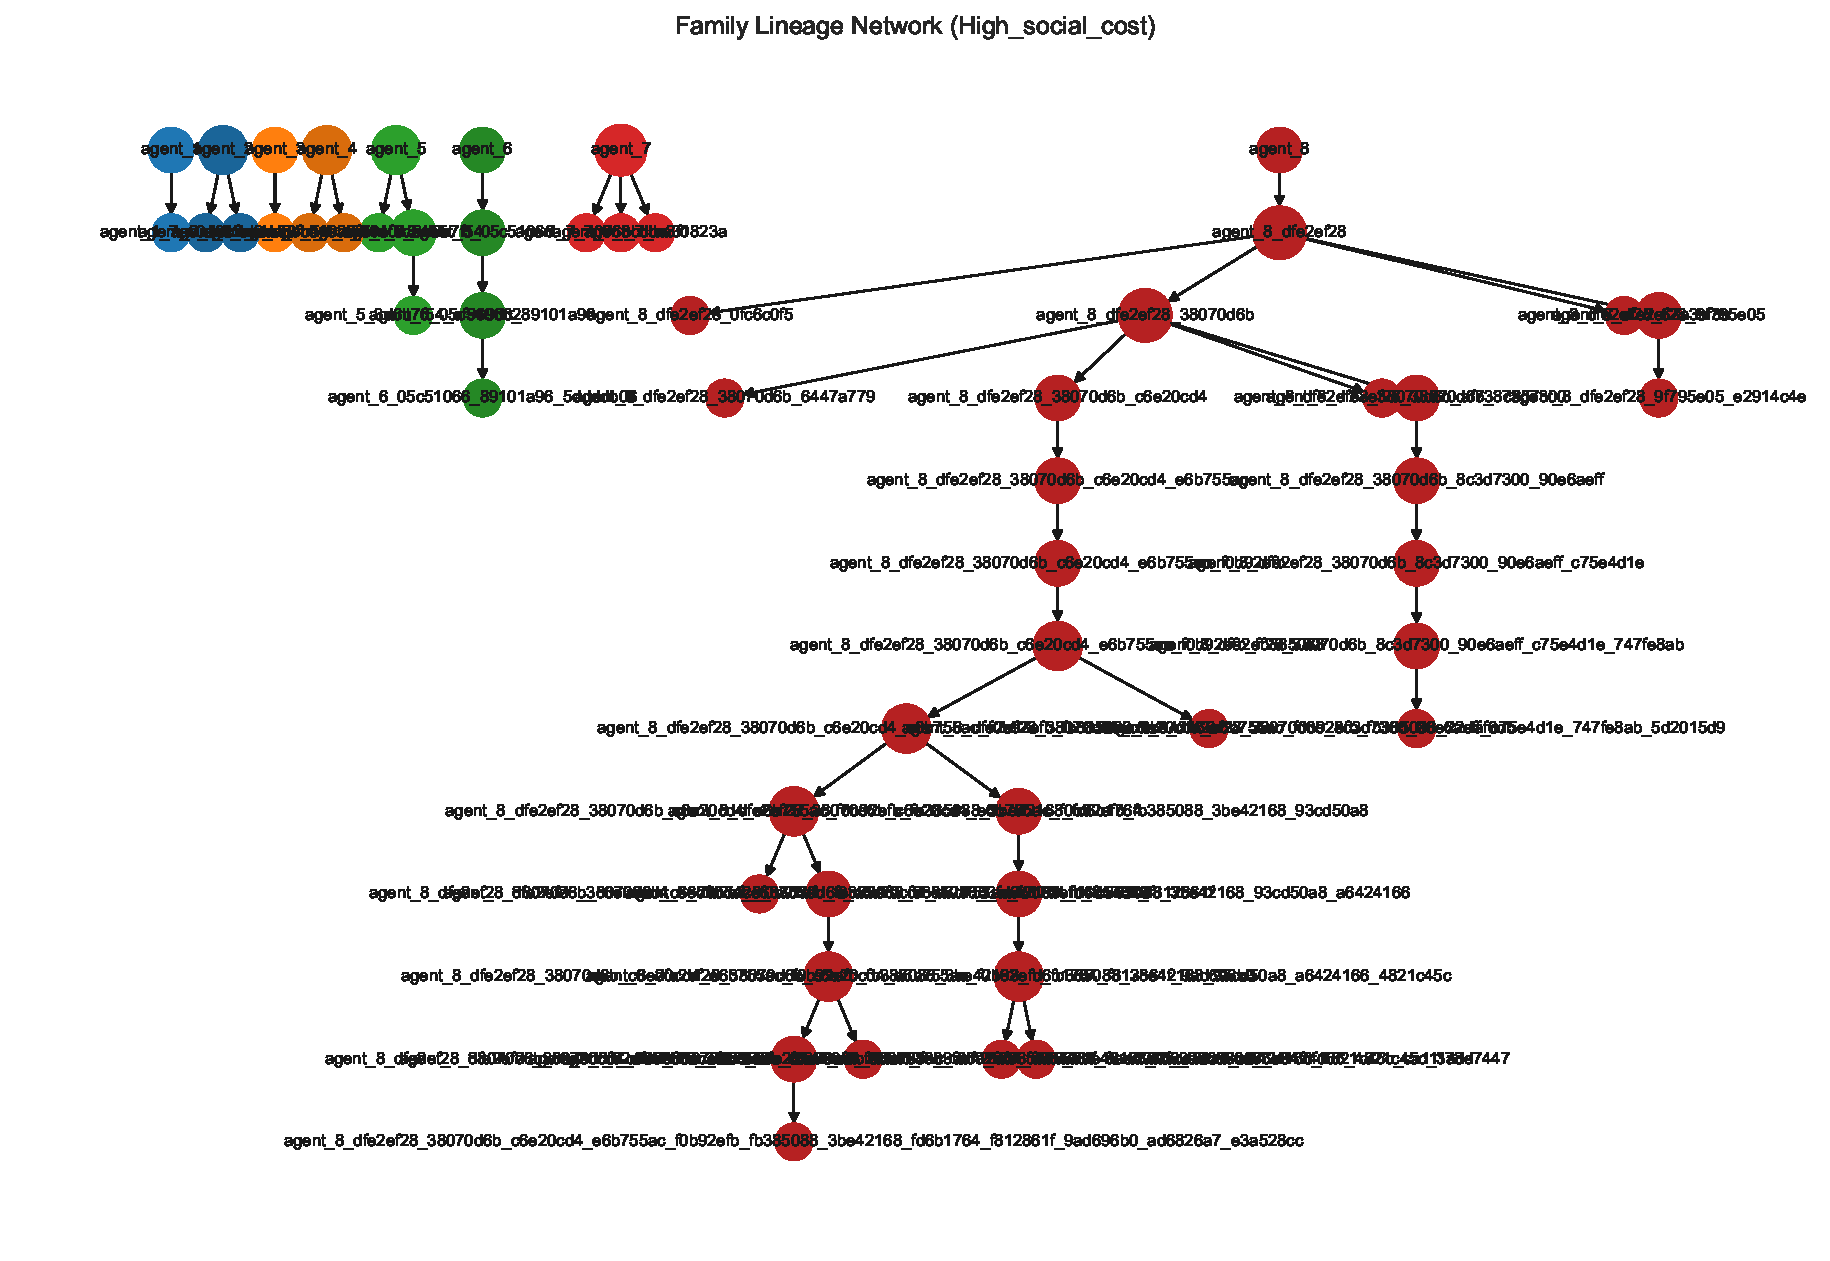
\includegraphics[width=\linewidth]{appendix_figures/networks/family_network_High_social_cost.pdf}
    \caption{Family Lineage Network for High Social Cost}
    \label{fig: family network high social cost}
\end{figure}

\begin{figure}[H]
    \centering
        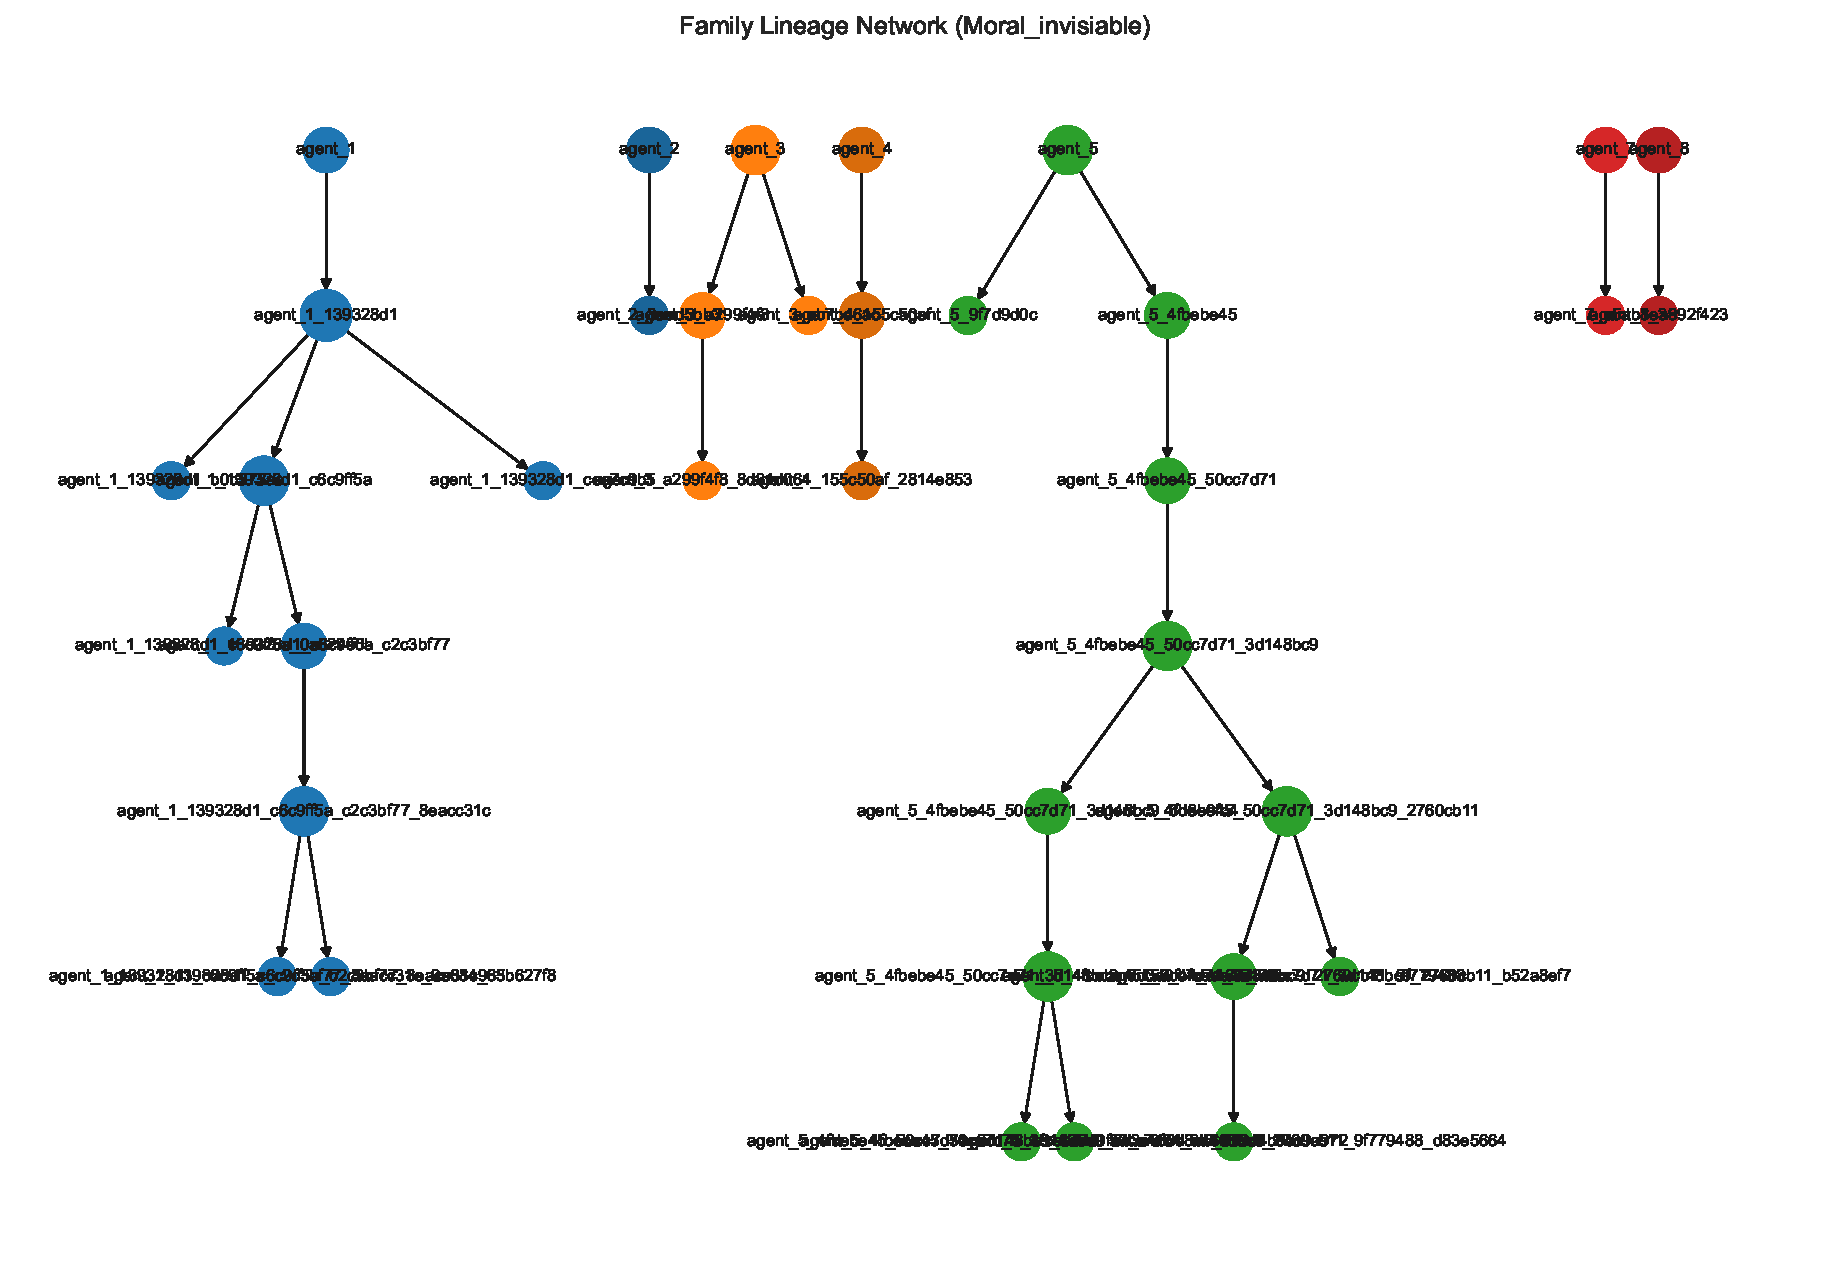
\includegraphics[width=\linewidth]{appendix_figures/networks/family_network_Moral_invisiable.pdf}
    \caption{Family Lineage Network for Moral Invisible}
    \label{fig: family network moral invisible}
\end{figure}

\begin{figure}[H]
    \centering
        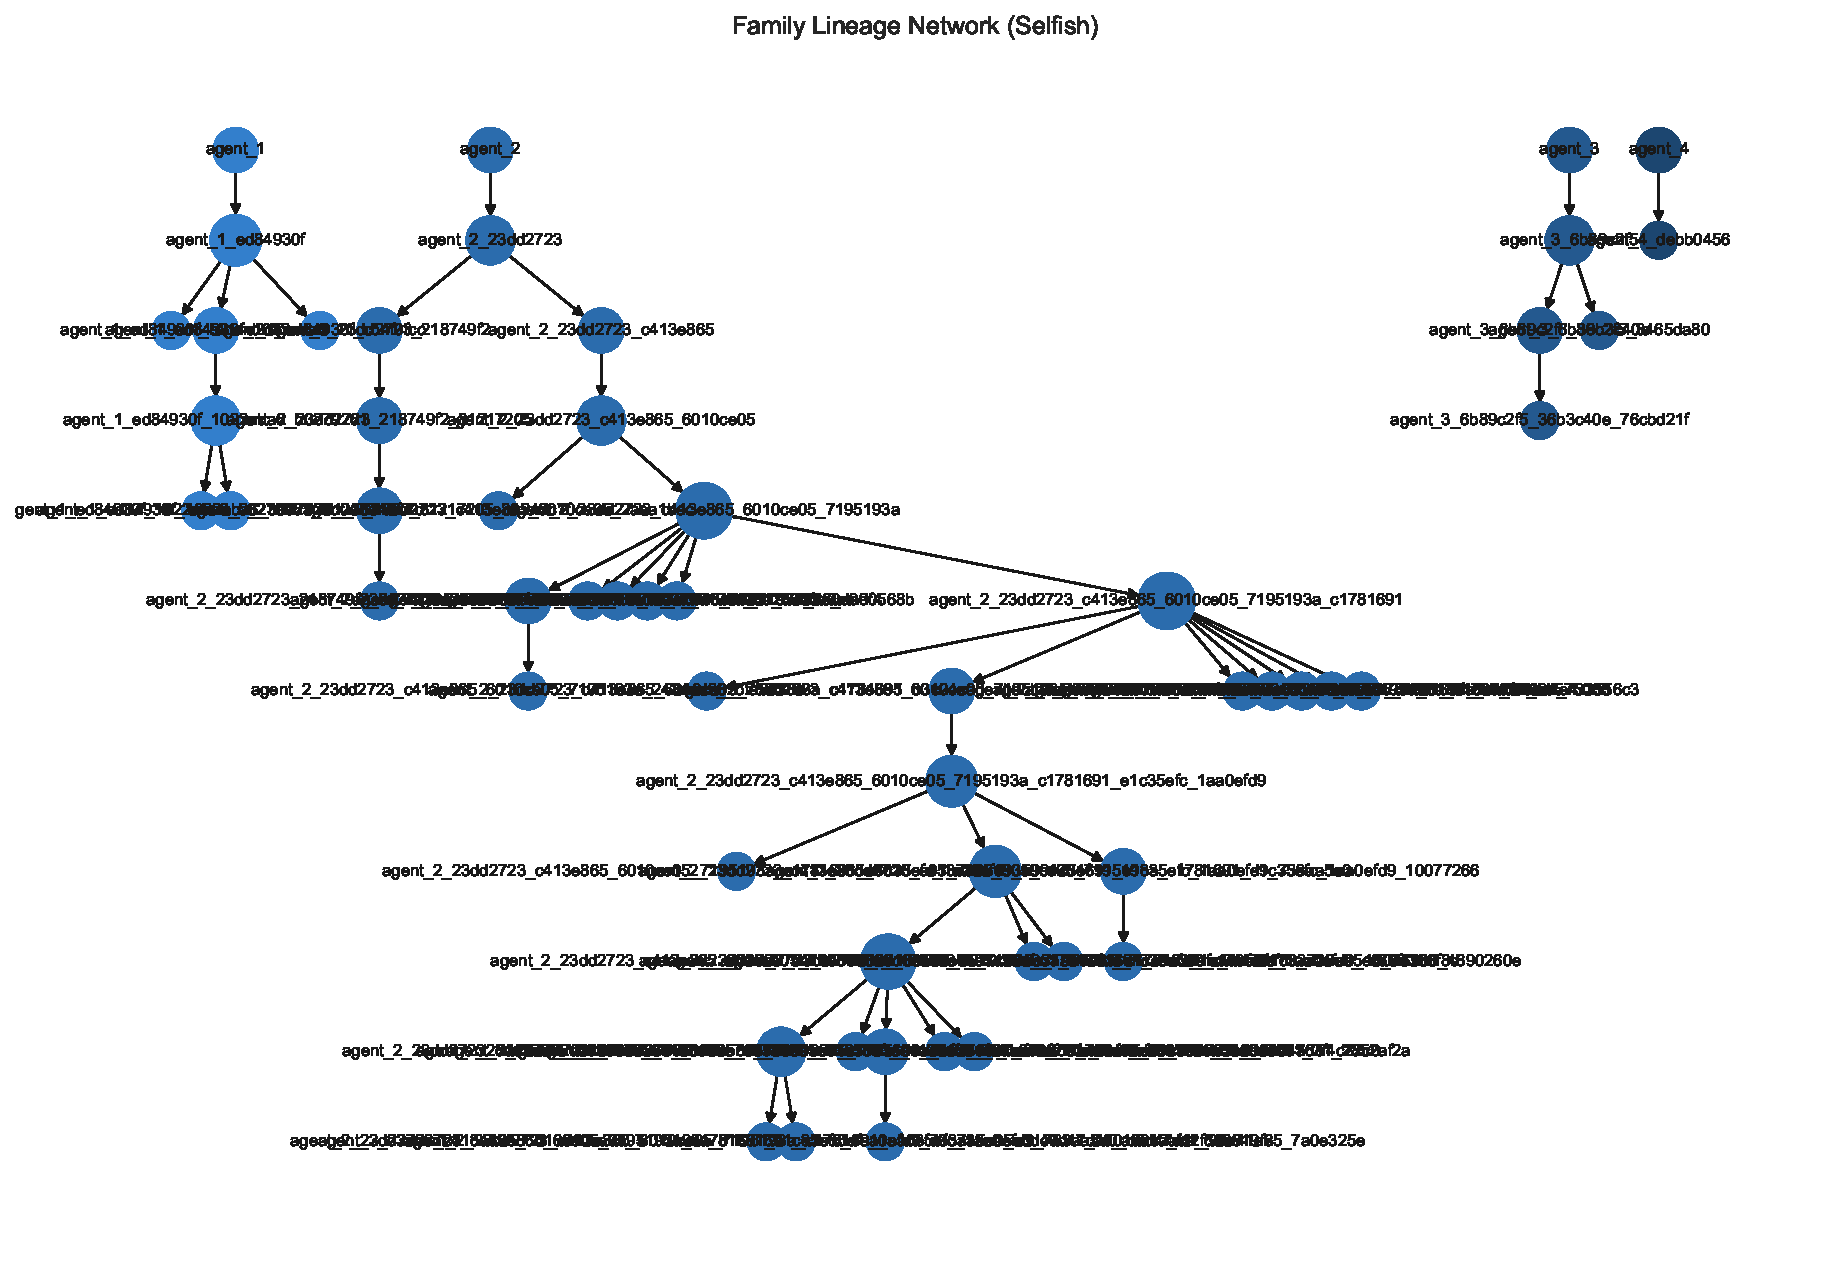
\includegraphics[width=\linewidth]{appendix_figures/networks/family_network_Selfish.pdf}
    \caption{Family Lineage Network for Selfish}
    \label{fig: family network selfish}
\end{figure}
    
\begin{figure}[H]
    \centering
        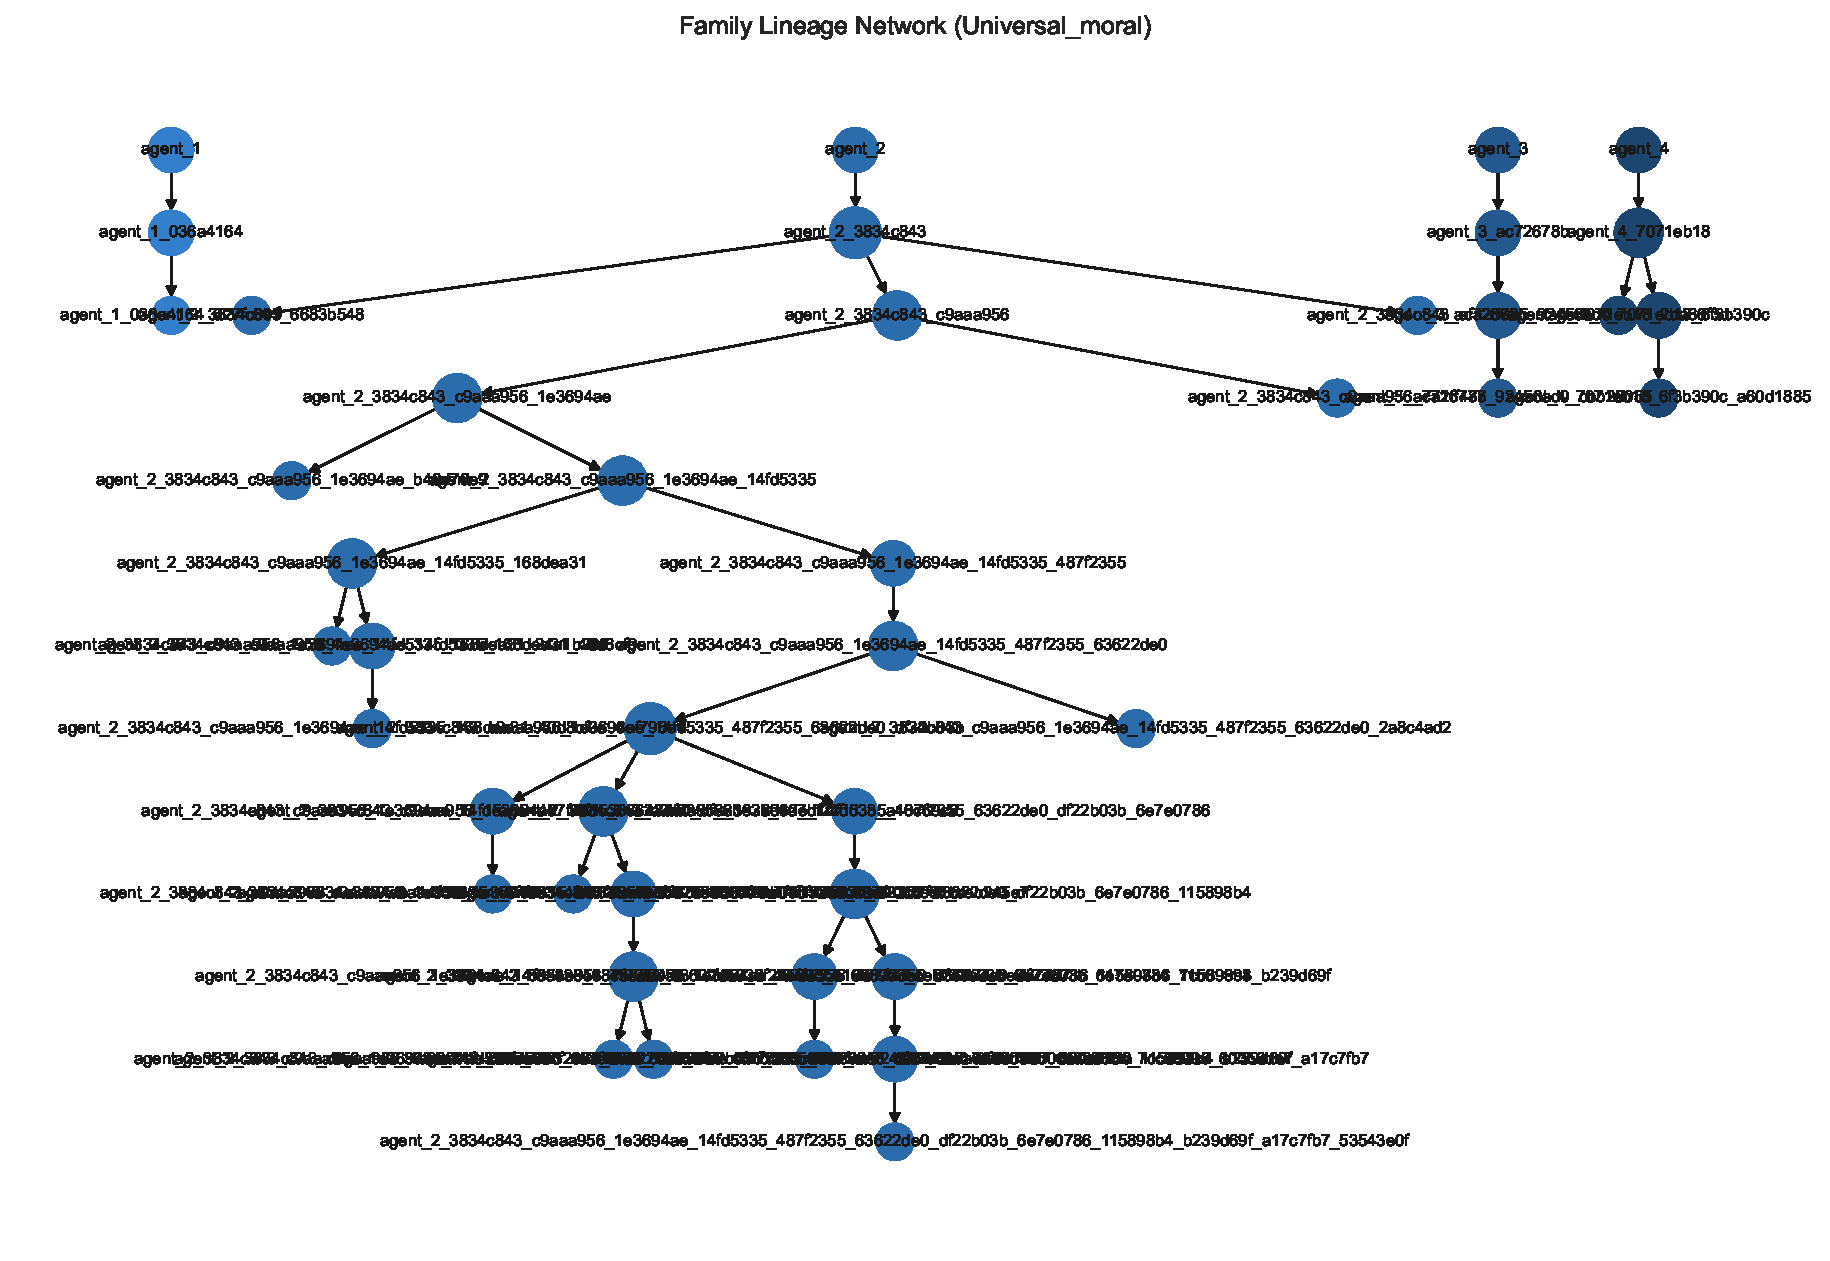
\includegraphics[width=\linewidth]{appendix_figures/networks/family_network_Universal_moral.pdf}
    \caption{Family Lineage Network for Universal Moral}
    \label{fig: family network universal}
\end{figure}

\begin{figure}[H]
    \centering
        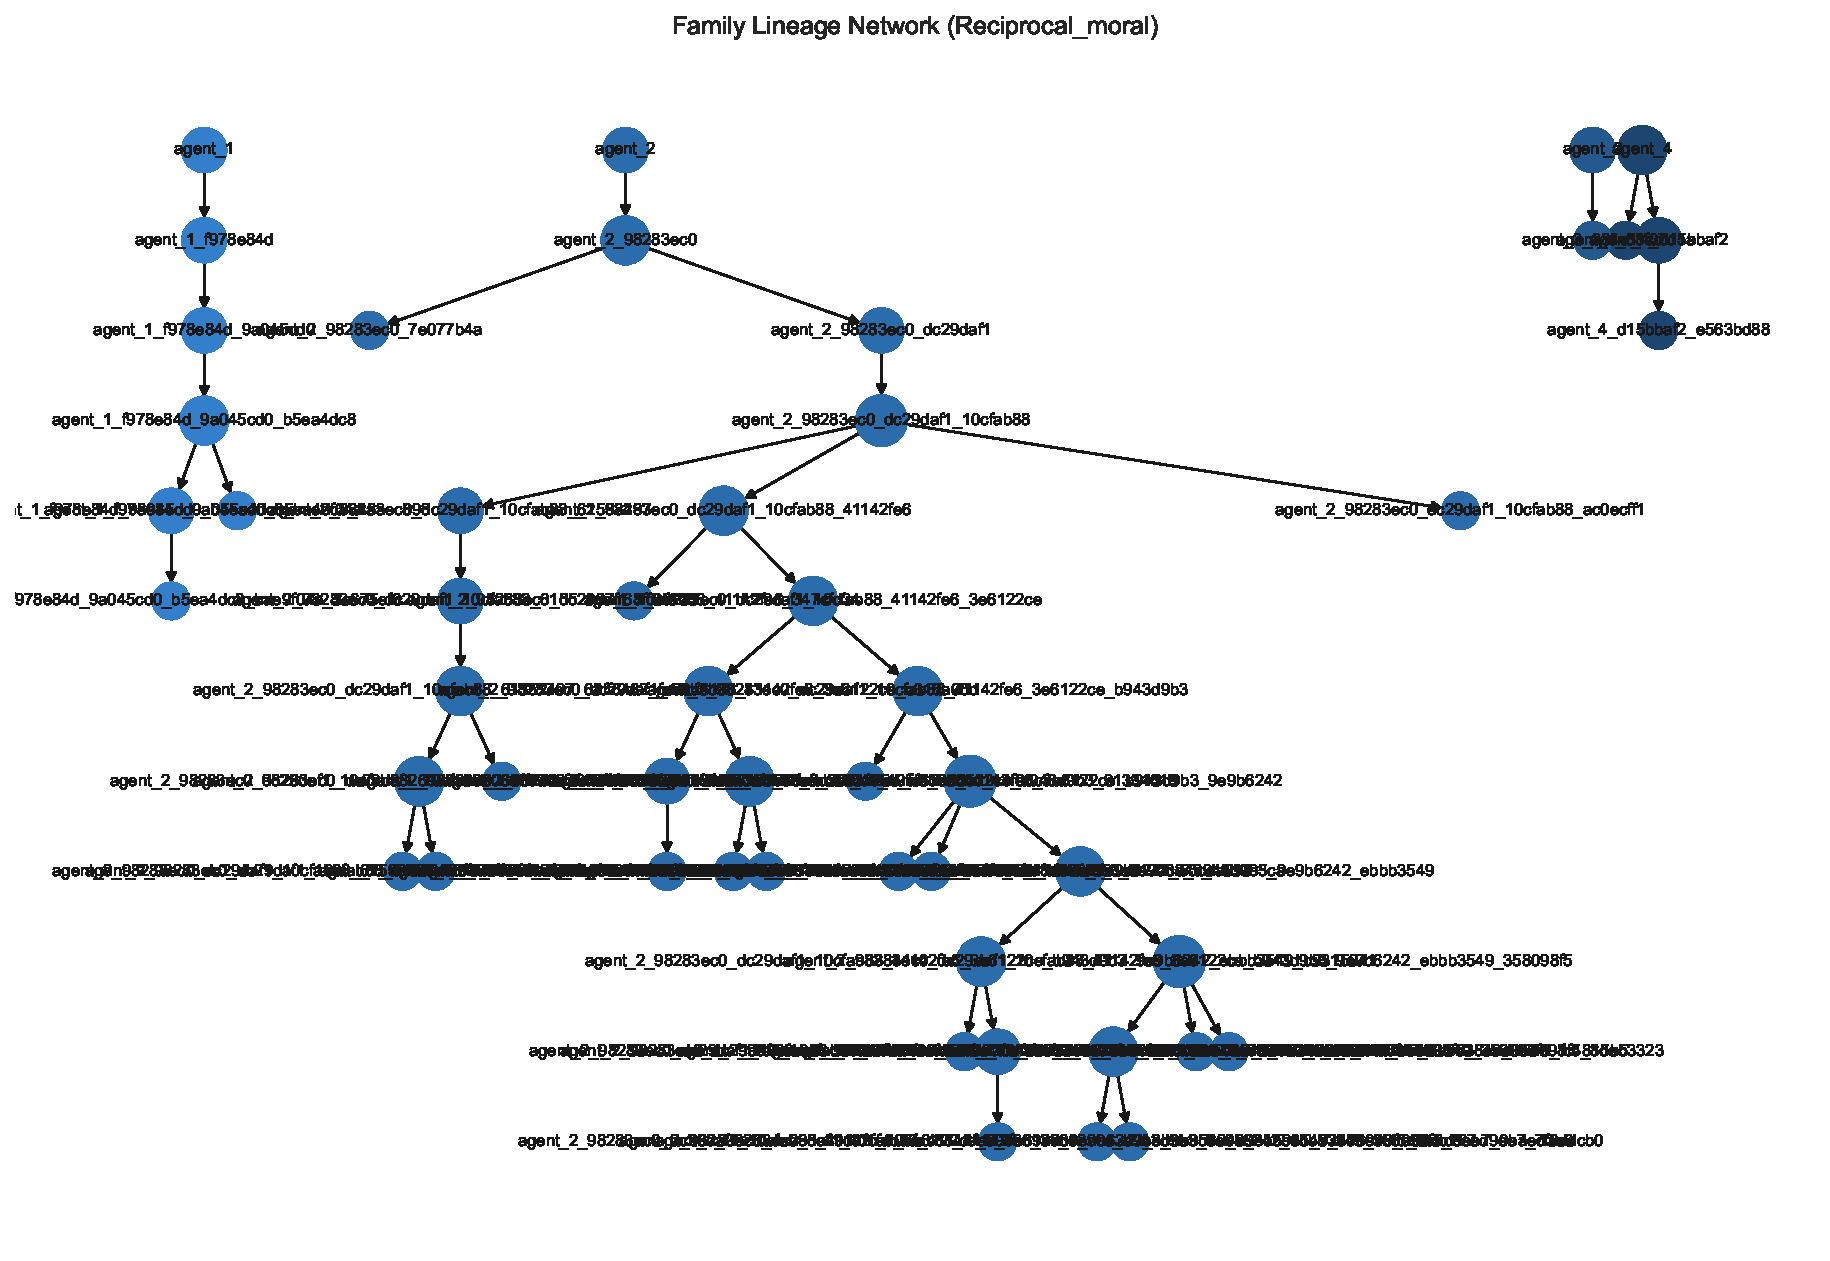
\includegraphics[width=\linewidth]{appendix_figures/networks/family_network_Reciprocal_moral.pdf}
    \caption{Family Lineage Network for Reciprocal Moral}
    \label{fig: family network reciprocal}
\end{figure}
    
\begin{figure}[H]
    \centering
        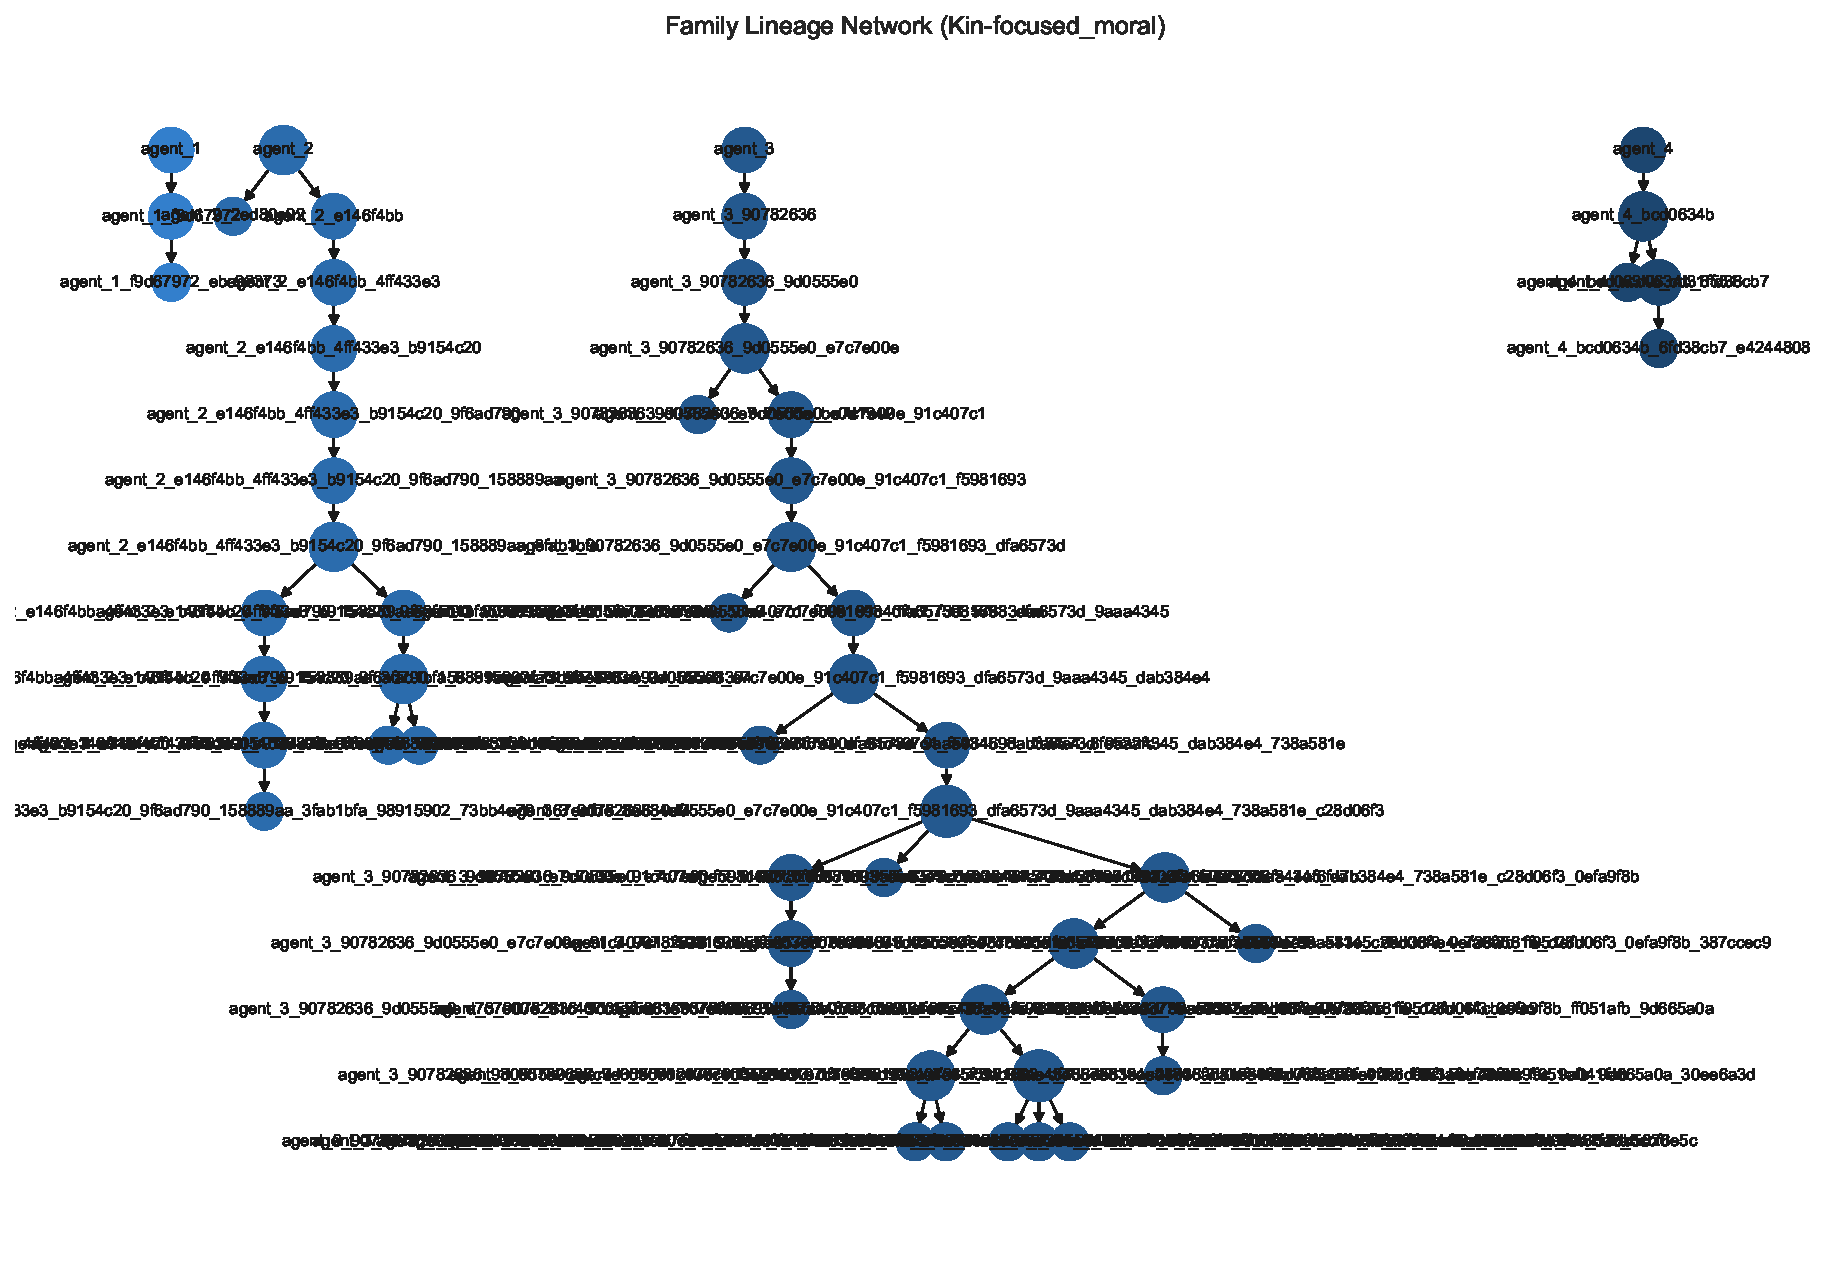
\includegraphics[width=\linewidth]{appendix_figures/networks/family_network_Kin-focused_moral.pdf}
    \caption{Family Lineage Network for Kin-focused Moral}
    \label{fig: family network kin}
\end{figure}


\subsubsection{Communication network}

Figures~\ref{fig: com network major} to \ref{fig: com network kin} depict the communication networks for agents under various scenarios. Each figure uses a network graph where nodes represent agents, and edges represent communication links. Edge thickness may indicate the frequency or strength of communication. Node colors and sizes may represent agent types or influence.

From all these figures, we could conclude that:
\begin{itemize}
    \item Occurred communications are scarce when communication is high and resources are scarce
    \item Universal moral and kin-focused moral agents in general have the most communication
\end{itemize}

\begin{figure}[H]
    \centering
        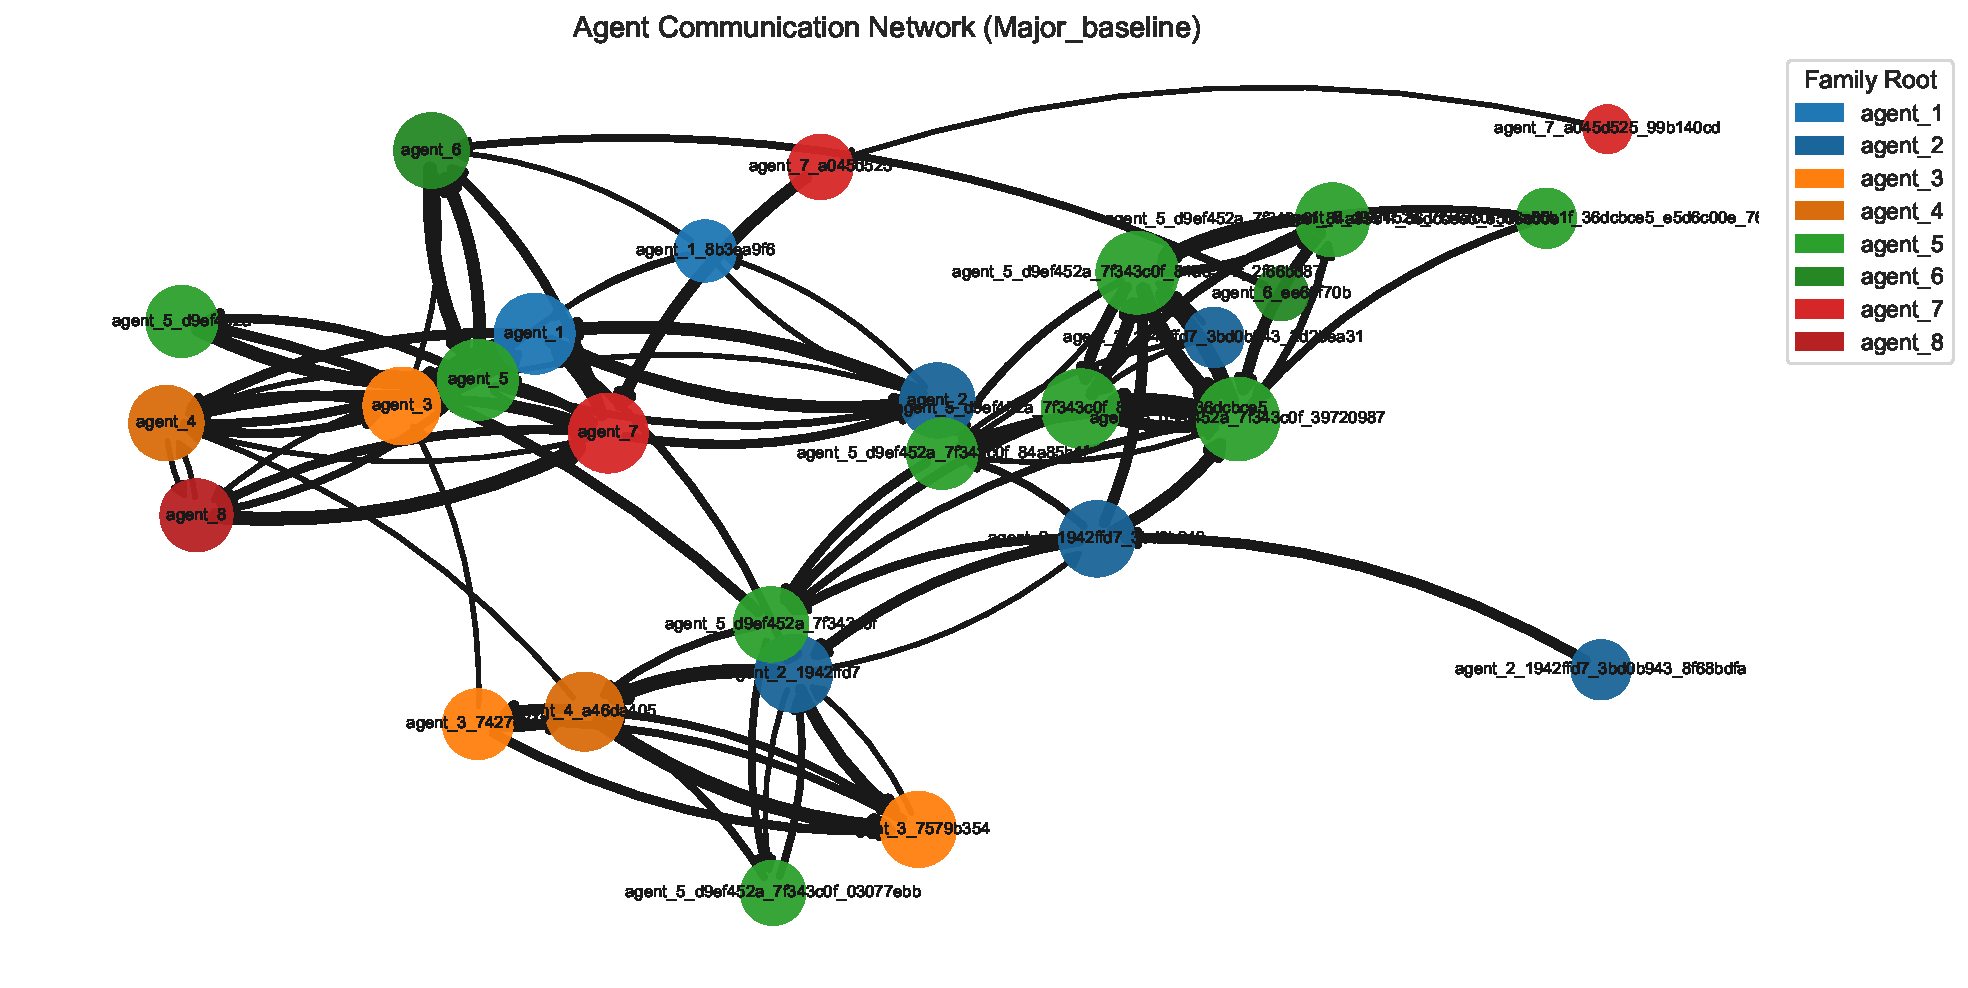
\includegraphics[width=\linewidth]{appendix_figures/networks/communication_network_Major_baseline.pdf}
    \caption{Communication network for Major Baseline}
    \label{fig: com network major}
\end{figure}

\begin{figure}[H]
    \centering
        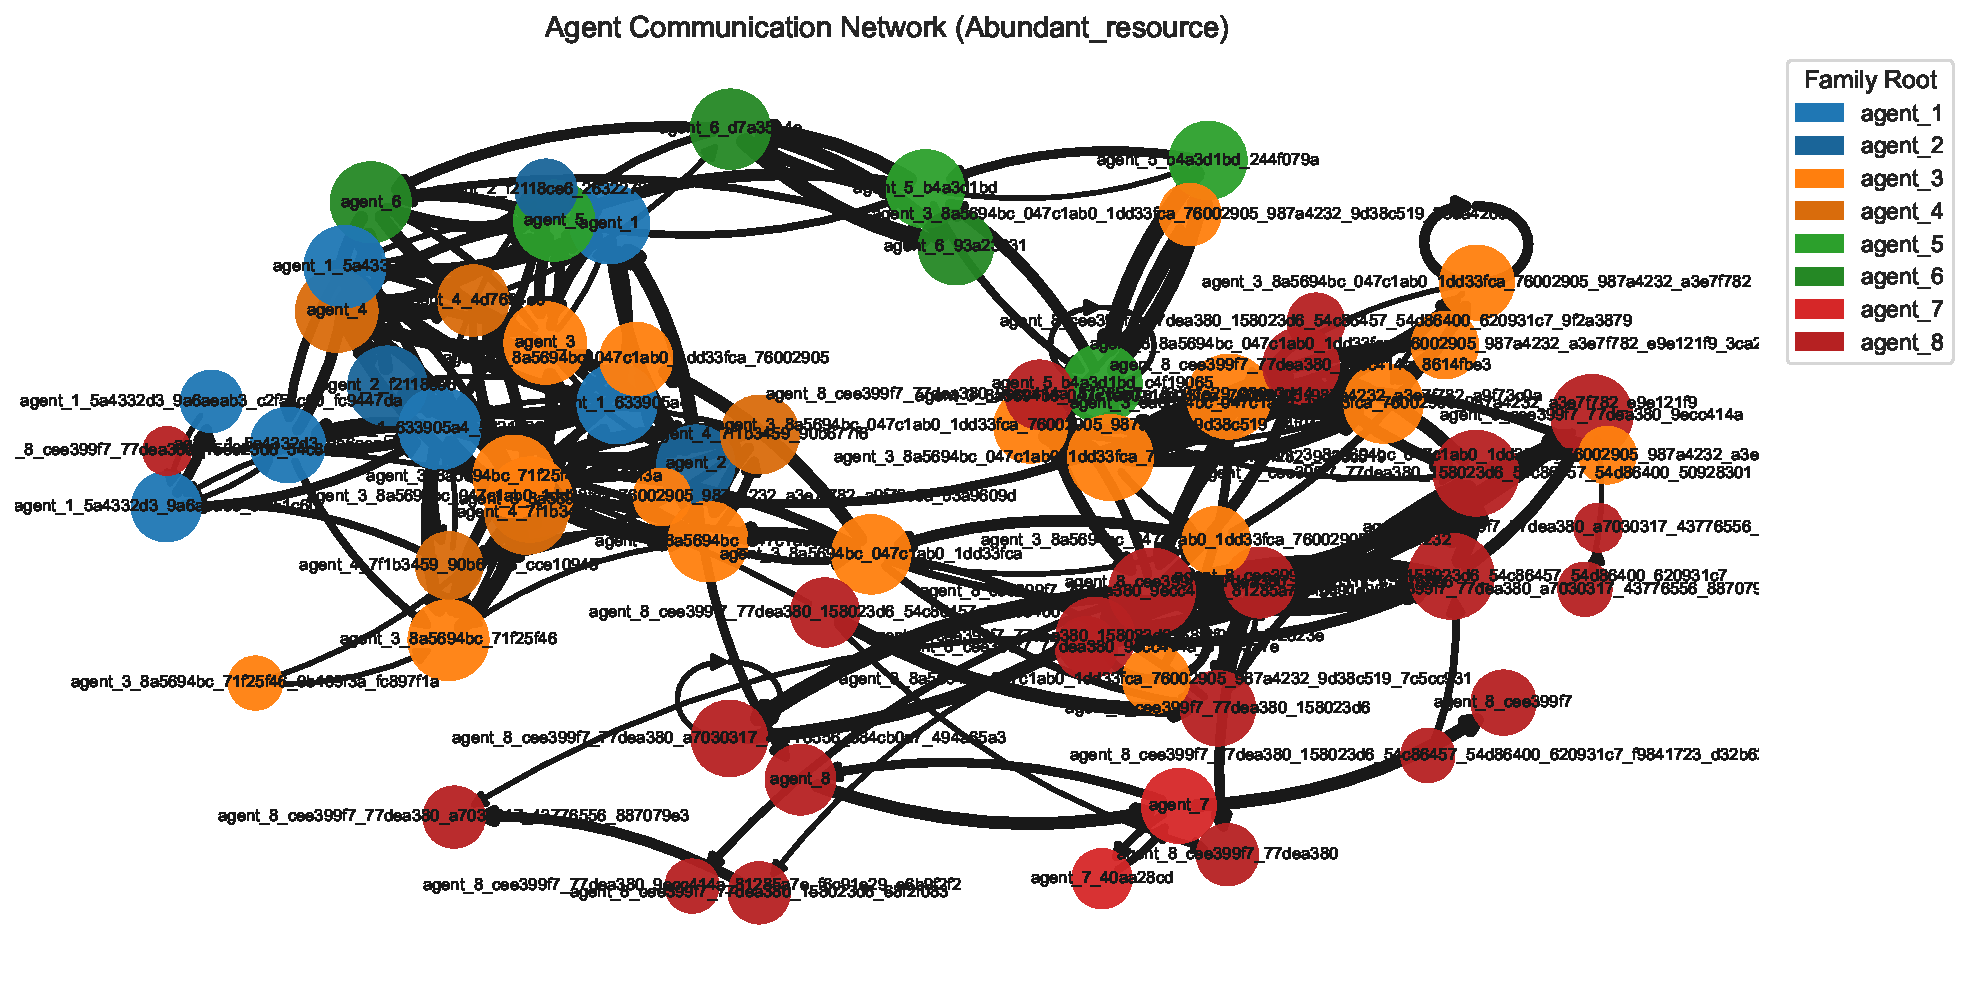
\includegraphics[width=\linewidth]{appendix_figures/networks/communication_network_Abundant_resource.pdf}
    \caption{Communication network for Abundant Resource}
    \label{fig: com network abundant}
\end{figure}
    
\begin{figure}[H]
    \centering   
        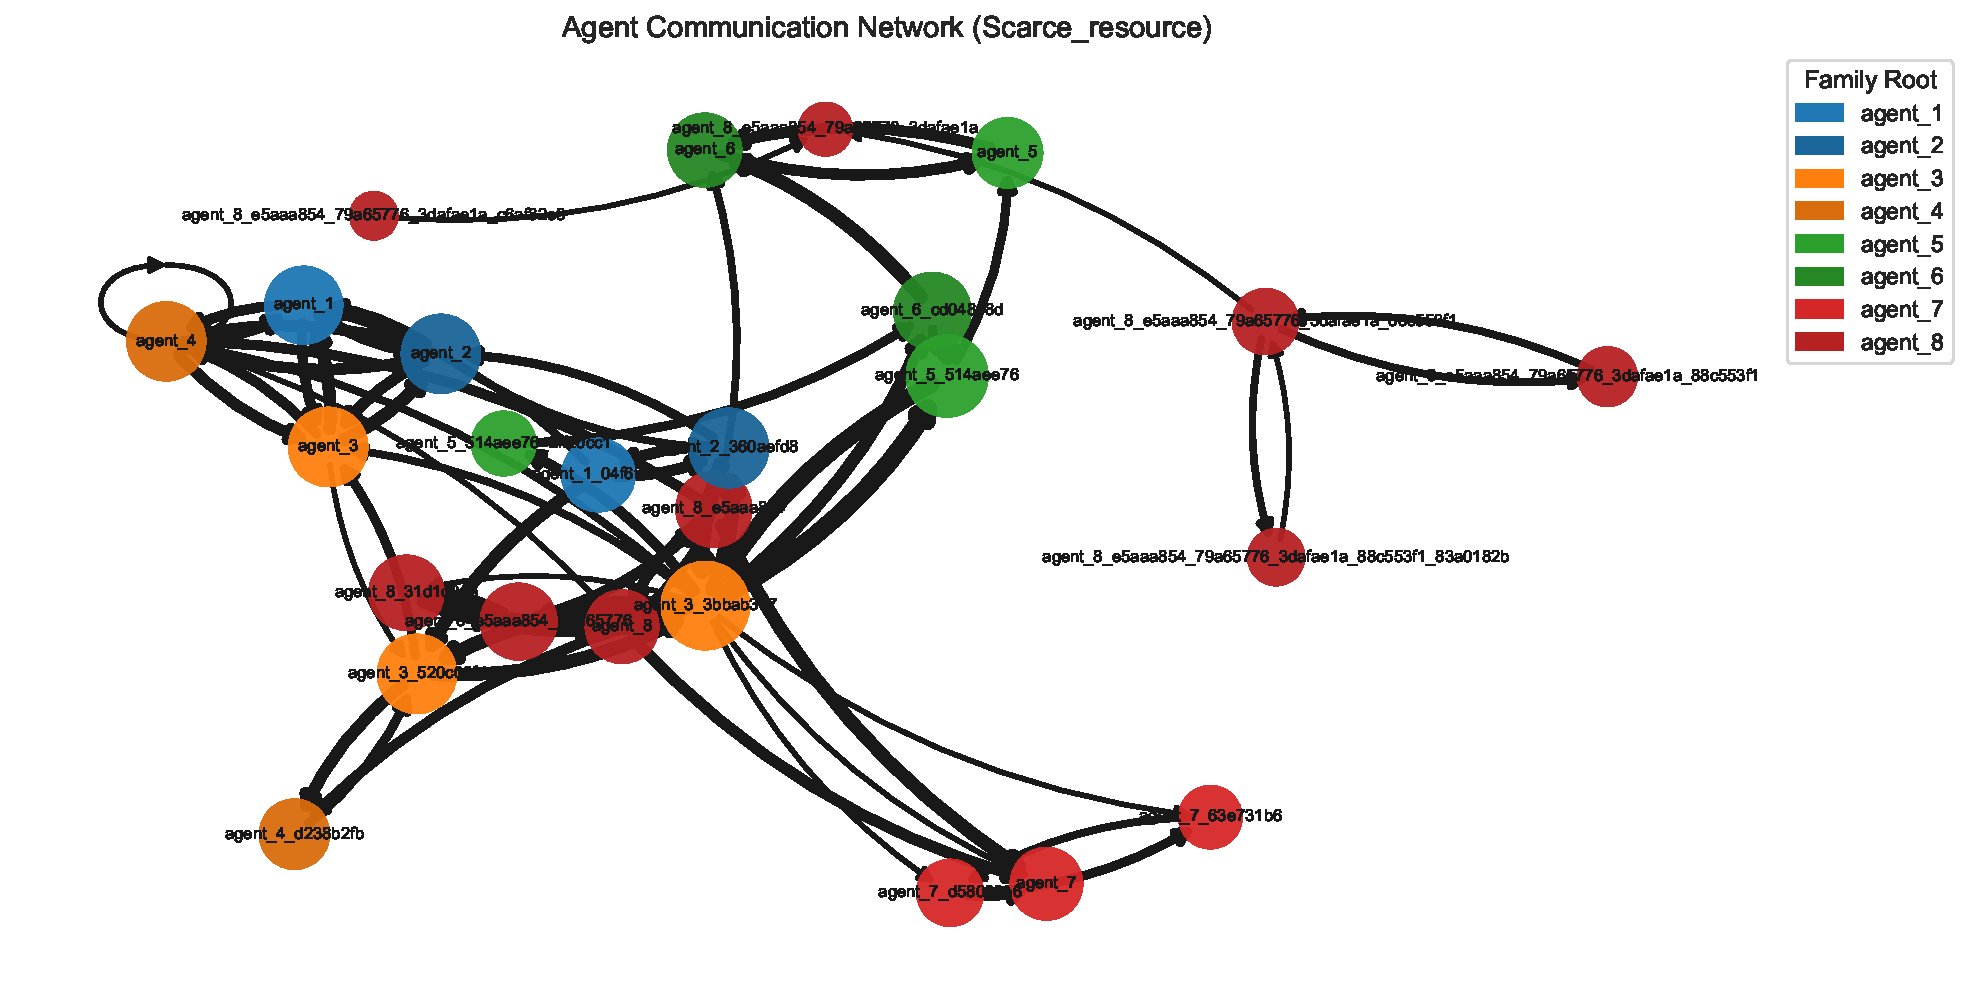
\includegraphics[width=\linewidth]{appendix_figures/networks/communication_network_Scarce_resource.pdf}
    \caption{Communication network for Scarce Resource}
    \label{fig: com network scarce}
\end{figure}

\begin{figure}[H]
    \centering
        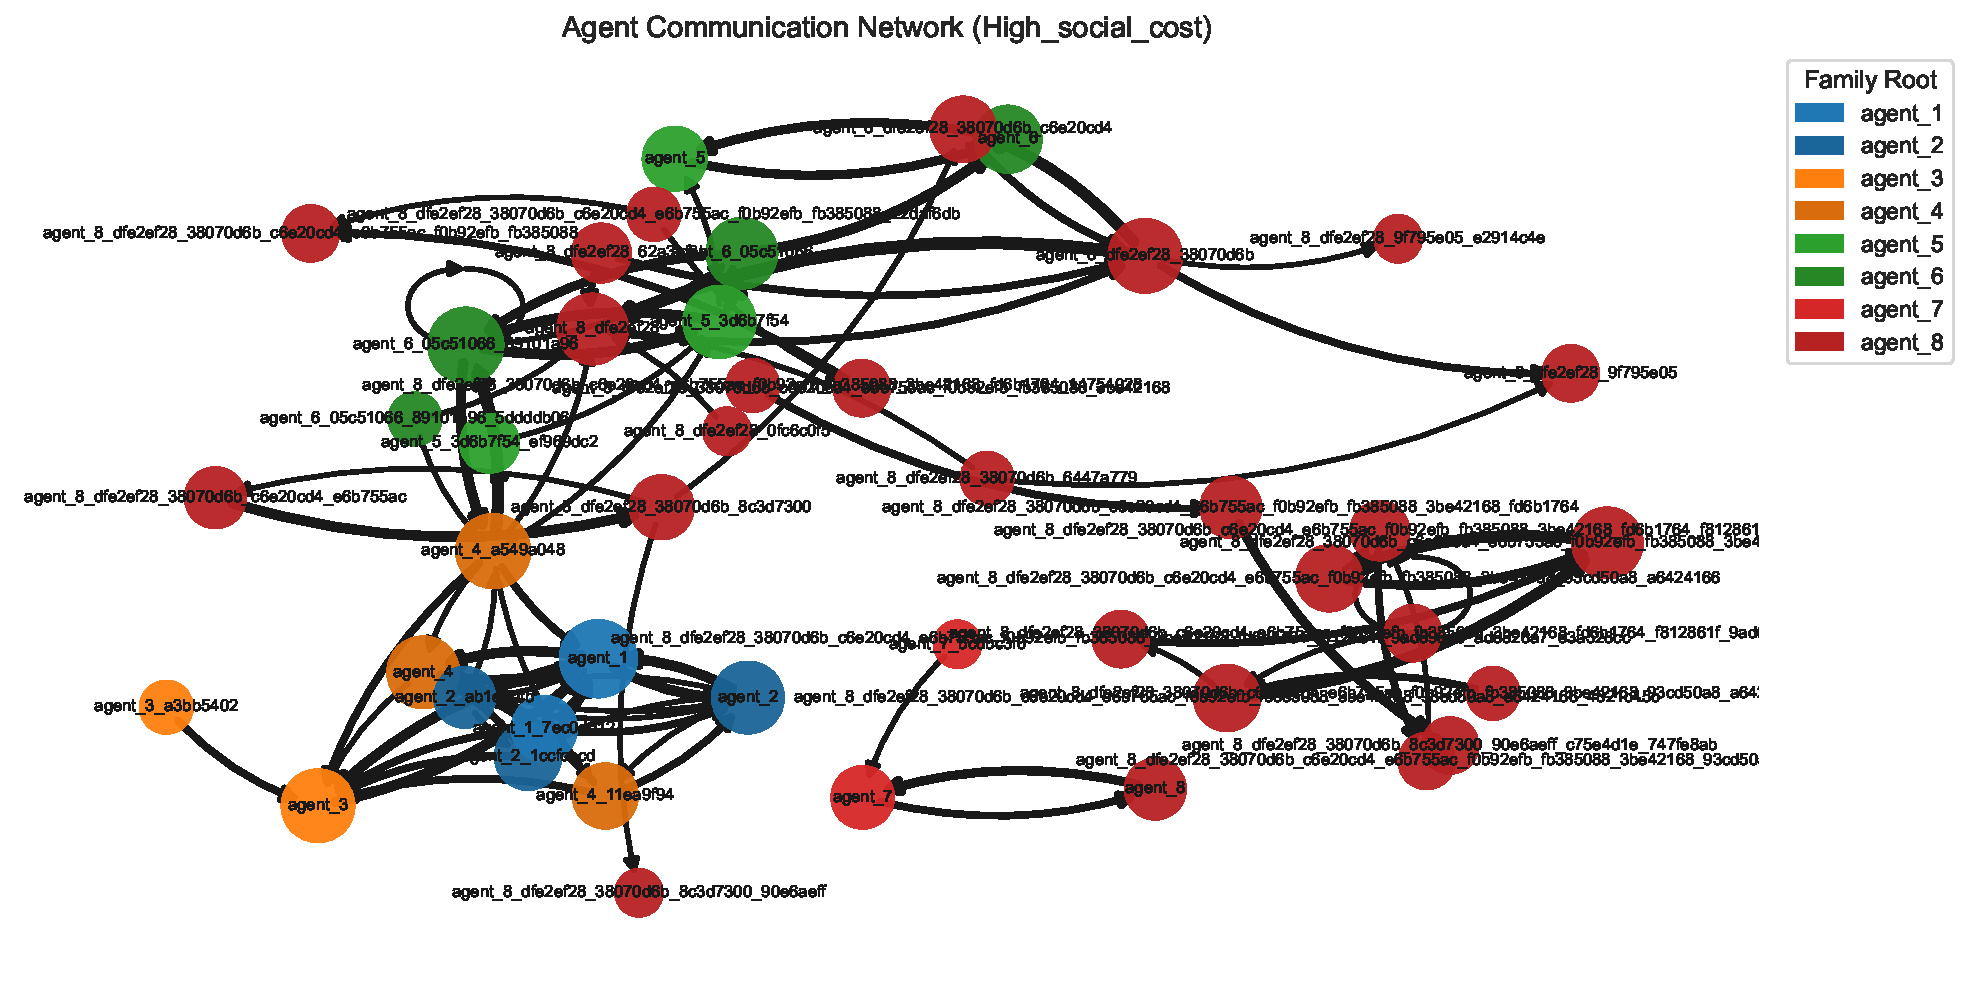
\includegraphics[width=\linewidth]{appendix_figures/networks/communication_network_High_social_cost.pdf}
    \caption{Communication network for High Social Cost}
    \label{fig: com network high social cost}
\end{figure}

\begin{figure}[H]
    \centering
        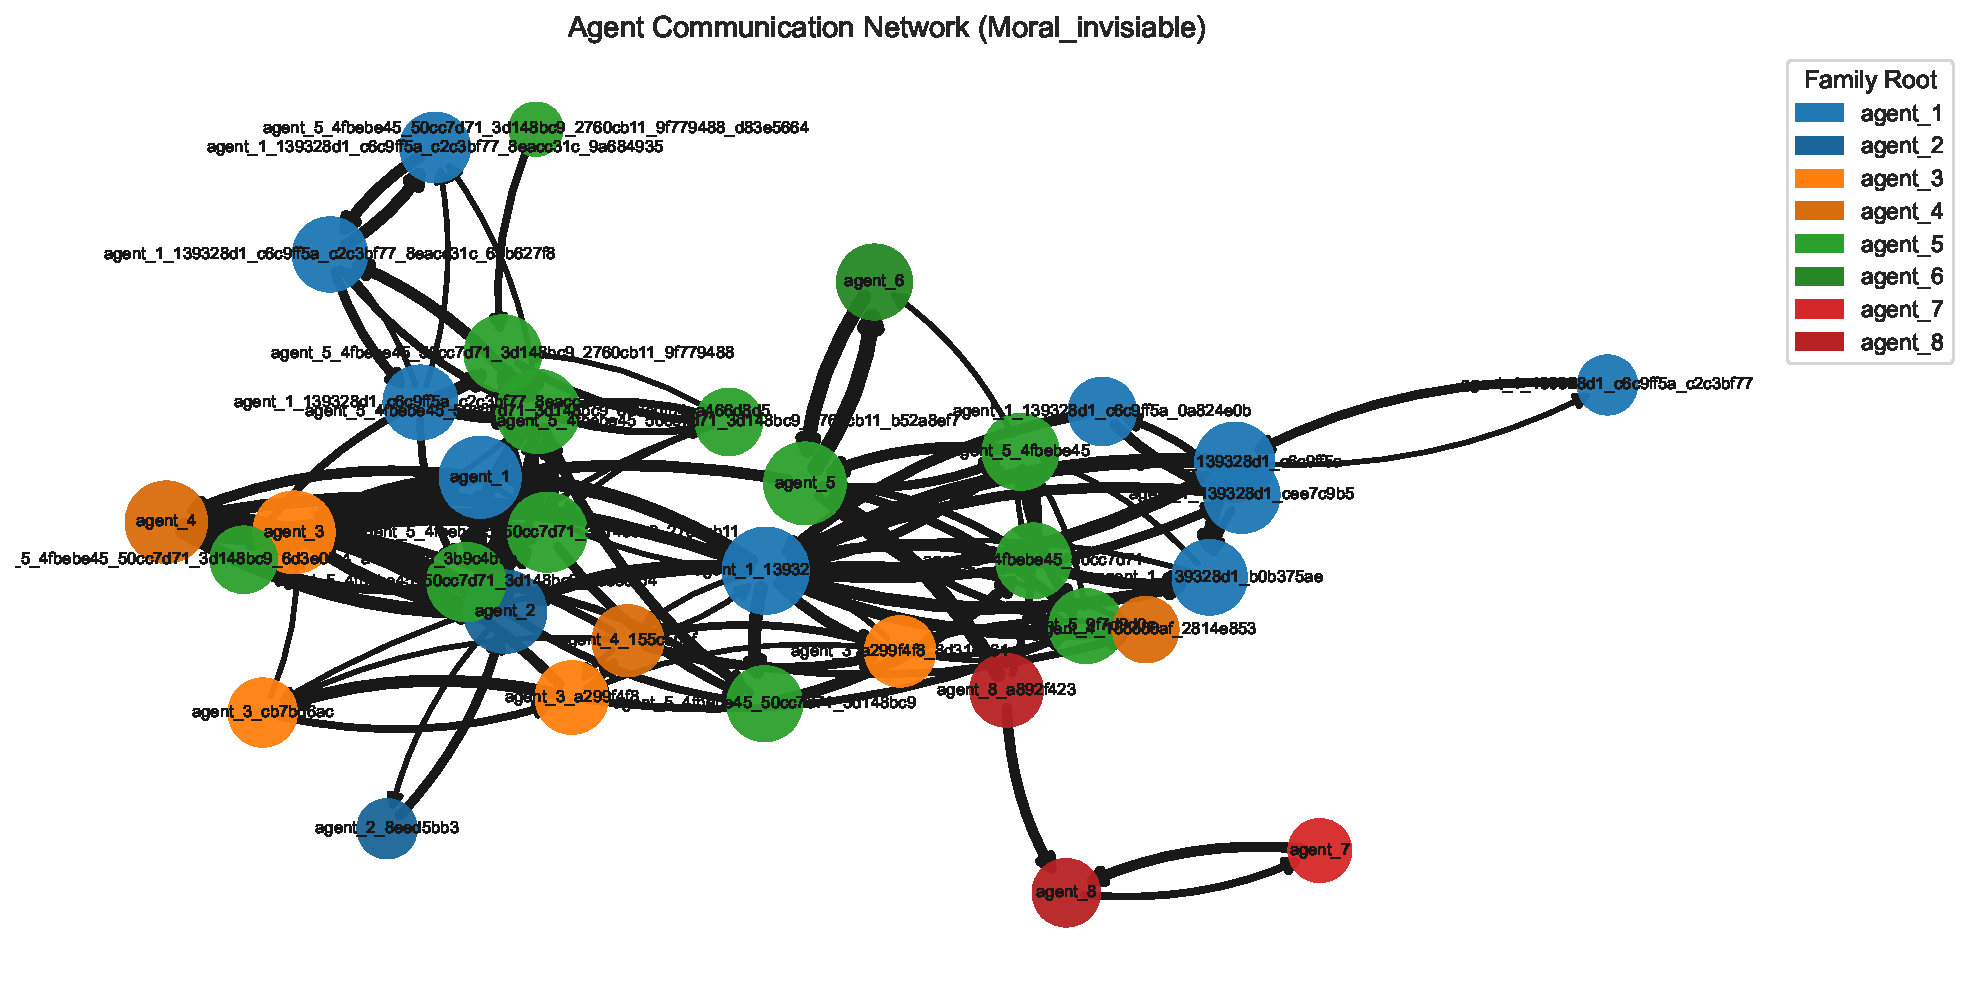
\includegraphics[width=\linewidth]{appendix_figures/networks/communication_network_Moral_invisiable.pdf}
    \caption{Communication network for Moral Invisible}
    \label{fig: com network moral invisible}
\end{figure}

\begin{figure}[H]
    \centering
        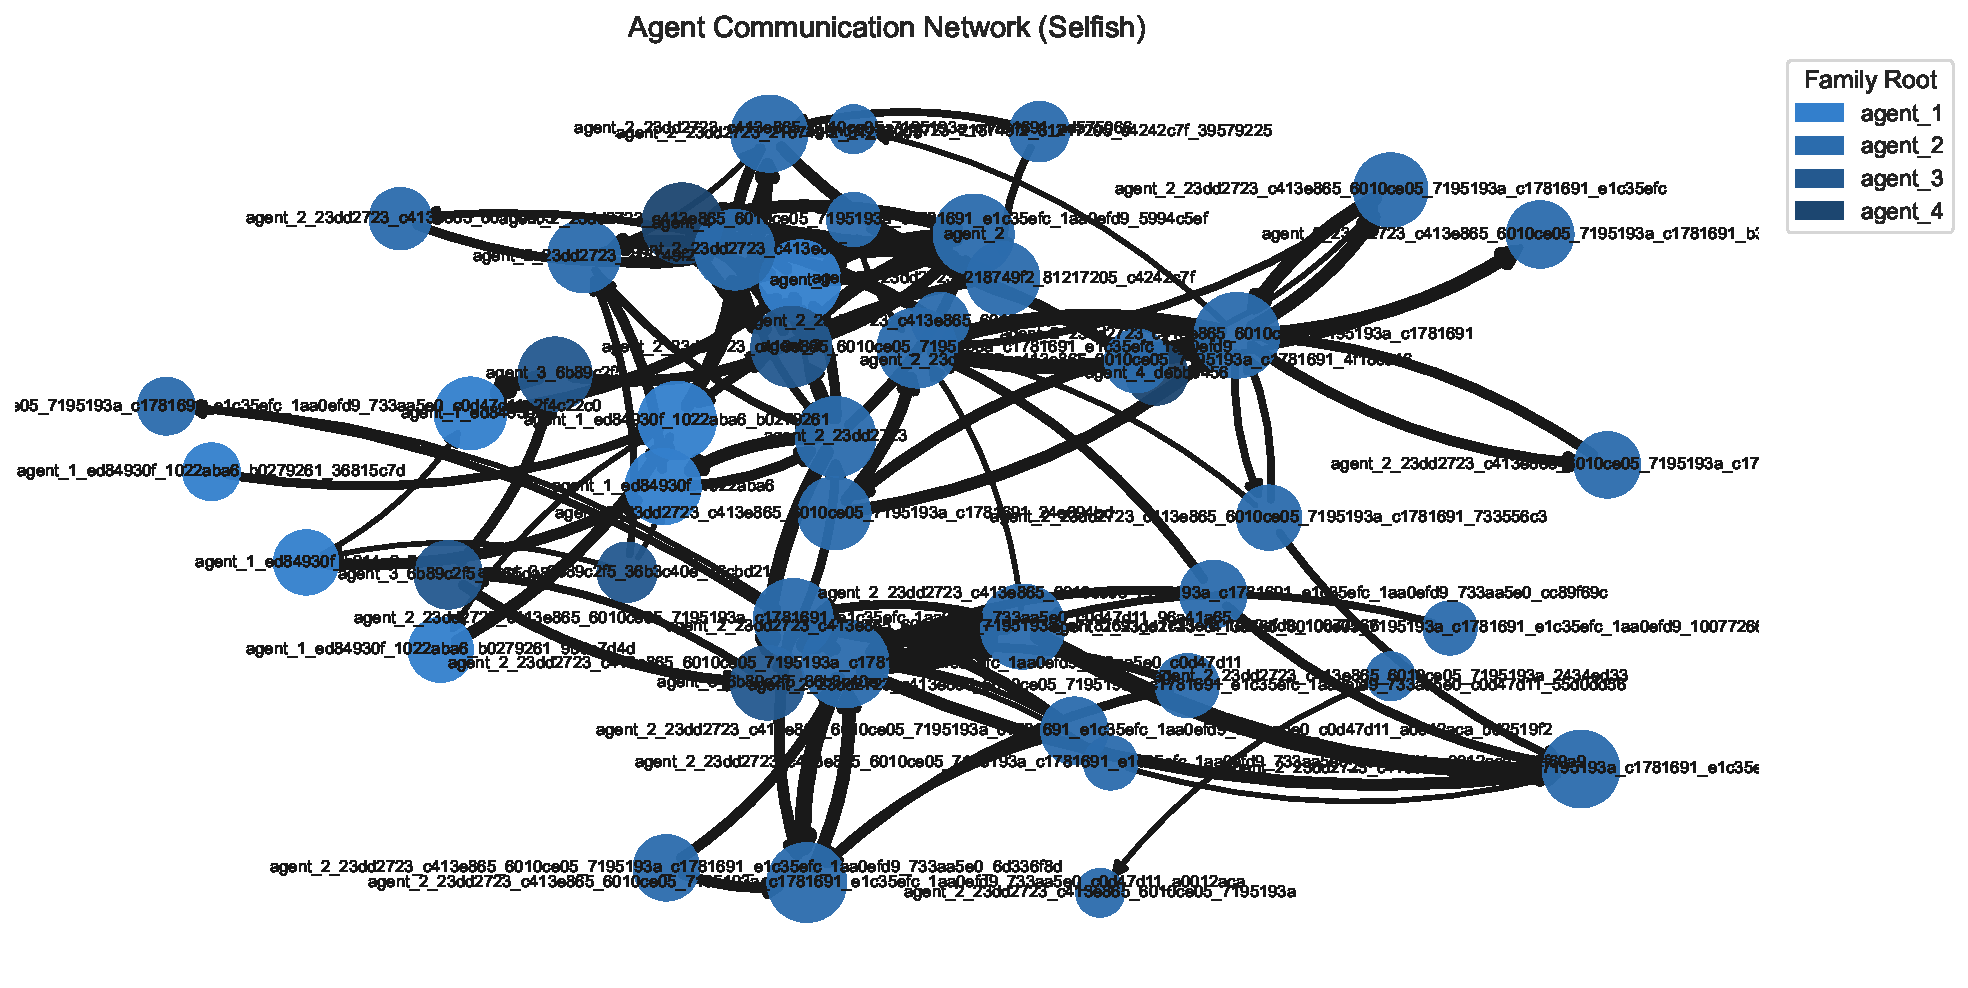
\includegraphics[width=\linewidth]{appendix_figures/networks/communication_network_Selfish.pdf}
    \caption{Communication network for Selfish}
    \label{fig: com network selfish}
\end{figure}
    
\begin{figure}[H]
    \centering
        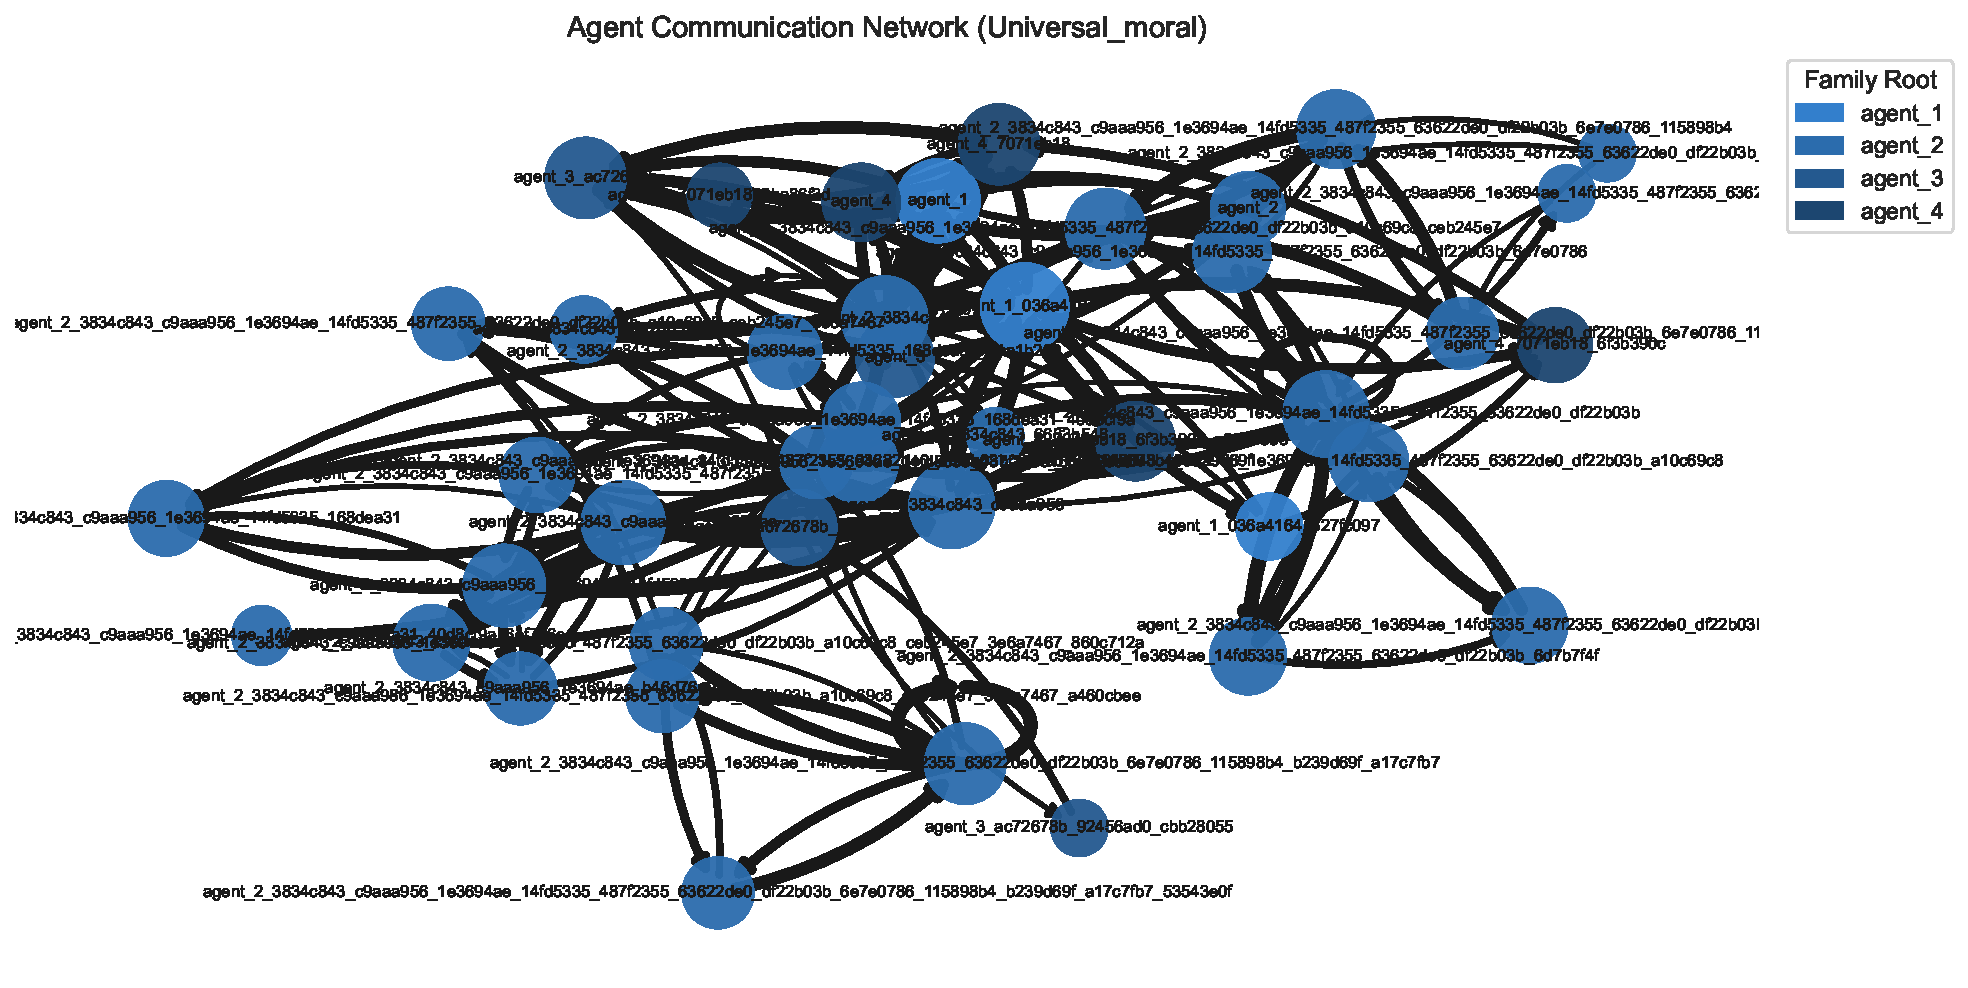
\includegraphics[width=\linewidth]{appendix_figures/networks/communication_network_Universal_moral.pdf}
    \caption{Communication network for Universal Moral}
    \label{fig: com network universal}
\end{figure}

\begin{figure}[H]
    \centering
        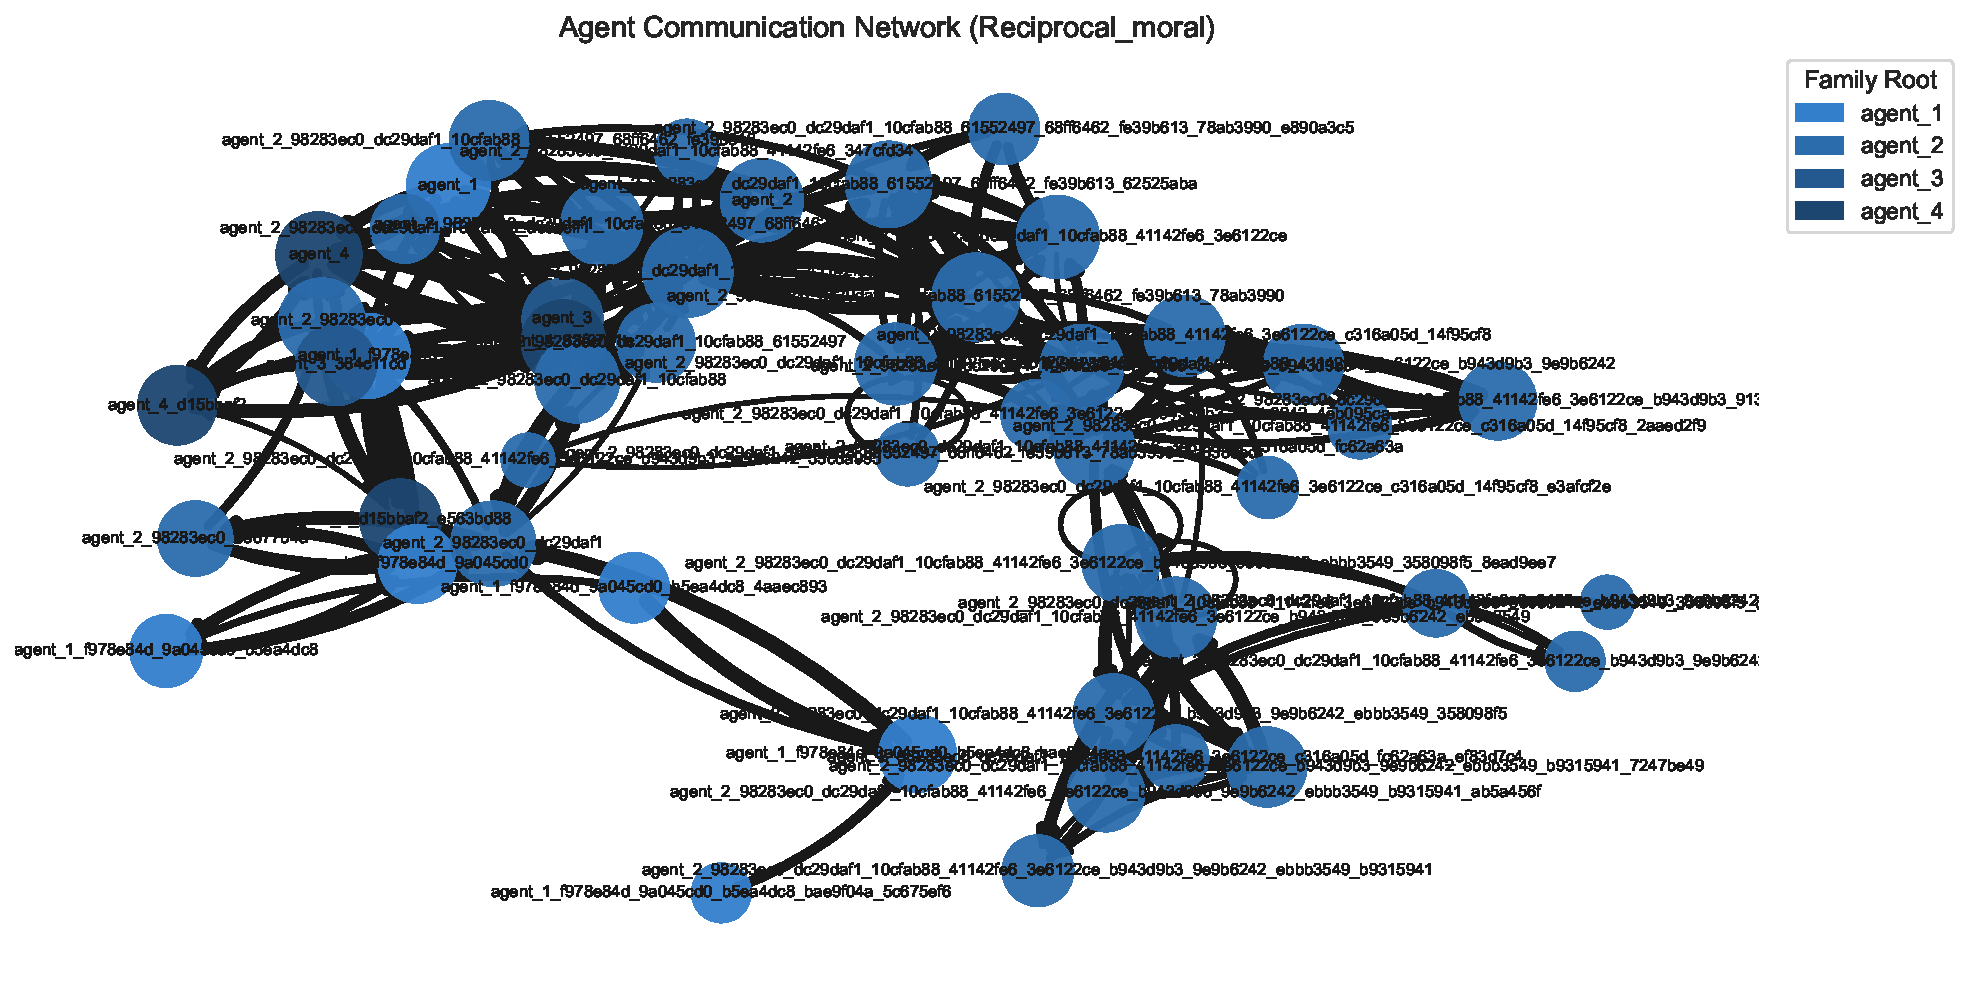
\includegraphics[width=\linewidth]{appendix_figures/networks/communication_network_Reciprocal_moral.pdf}
    \caption{Communication network for Reciprocal Moral}
    \label{fig: com network reciprocal}
\end{figure}
    
\begin{figure}[H]
    \centering
        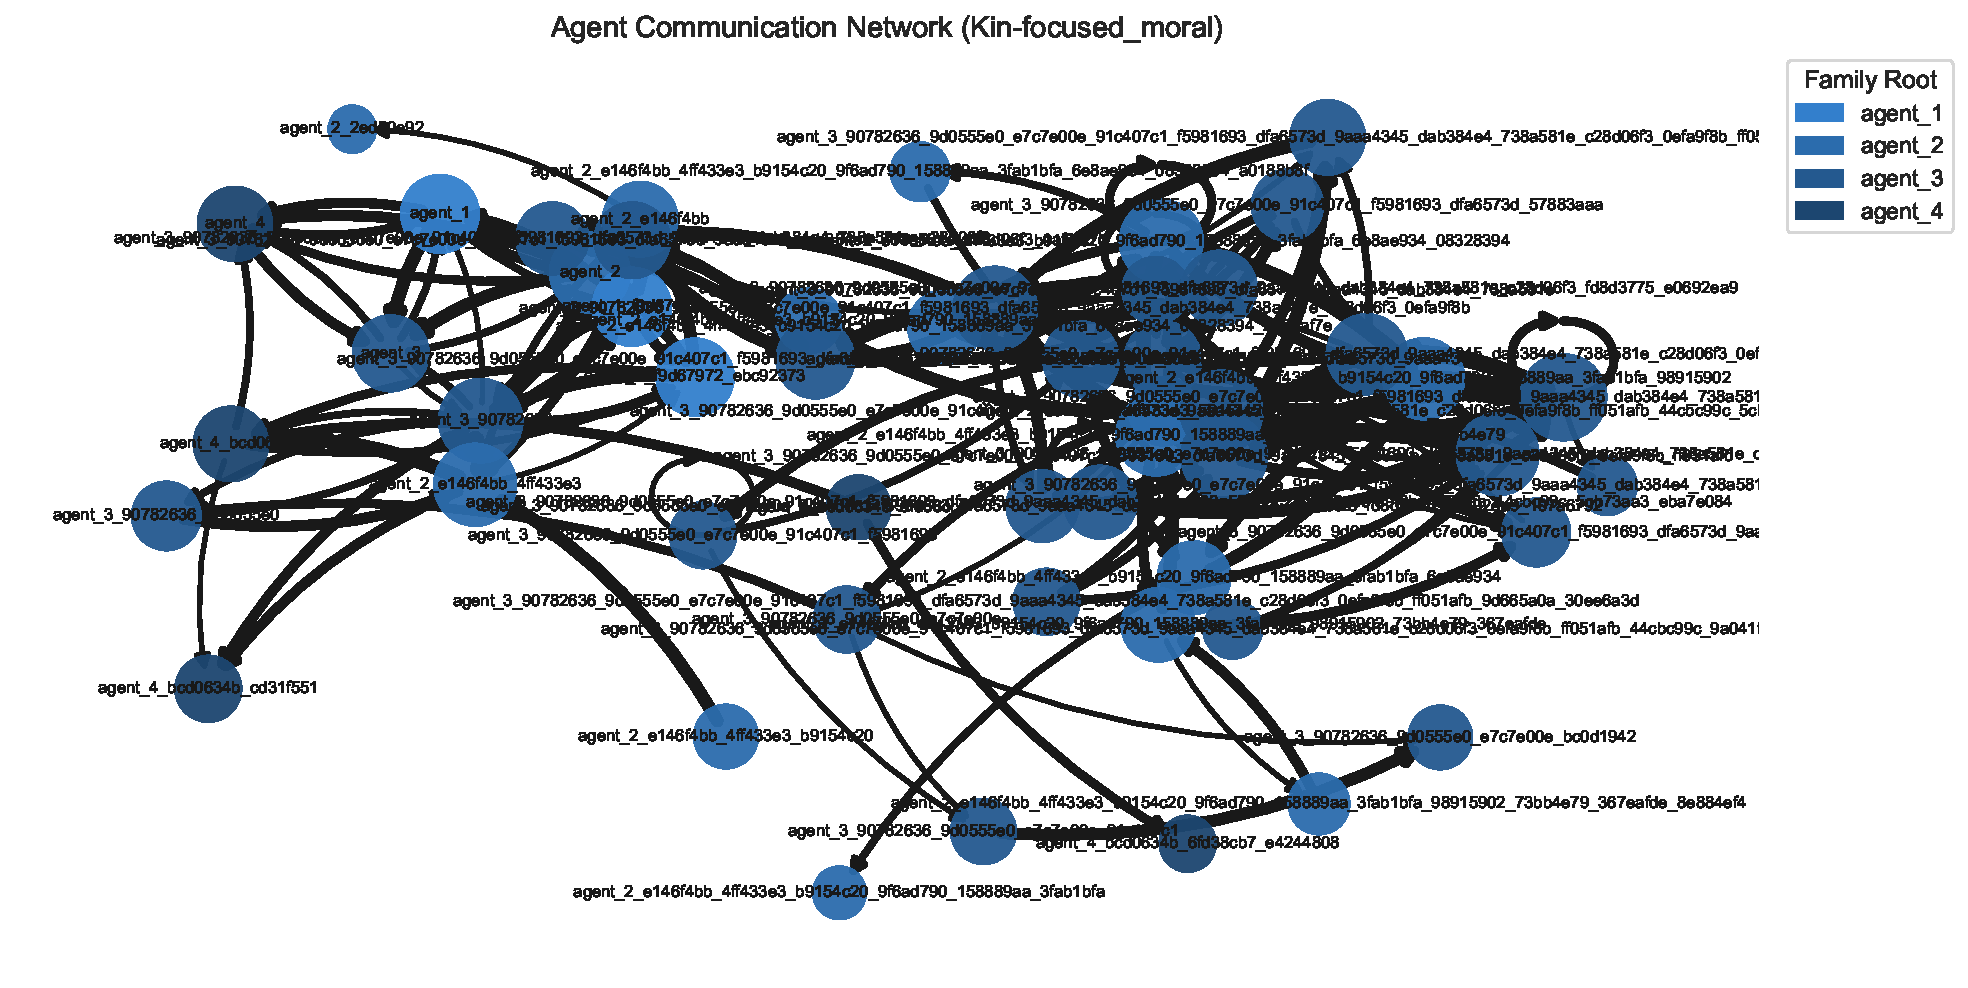
\includegraphics[width=\linewidth]{appendix_figures/networks/communication_network_Kin-focused_moral.pdf}
    \caption{Communication network for Kin-focused Moral}
    \label{fig: com network kin}
\end{figure}


\subsubsection{Selected hunt collaboration}

Figure~\ref{fig: hunt distribution main} illustrates the selected collaboration dynamics in the major baseline scenario. Each figure shows the distributions of the damages and HP allocation of a hunt. The x-axis represents the participant agents, while the y-axis represents the ratio of the damages that agents made, and the allocated HP from the killer agent.

From the figure, we noticed that in most scenarios, agents who kill the prey do not allocate the HP accordingly. In some cases, they did allocate based on their memory about their team instead of the real contribution.

\begin{figure}[H]
    \centering
    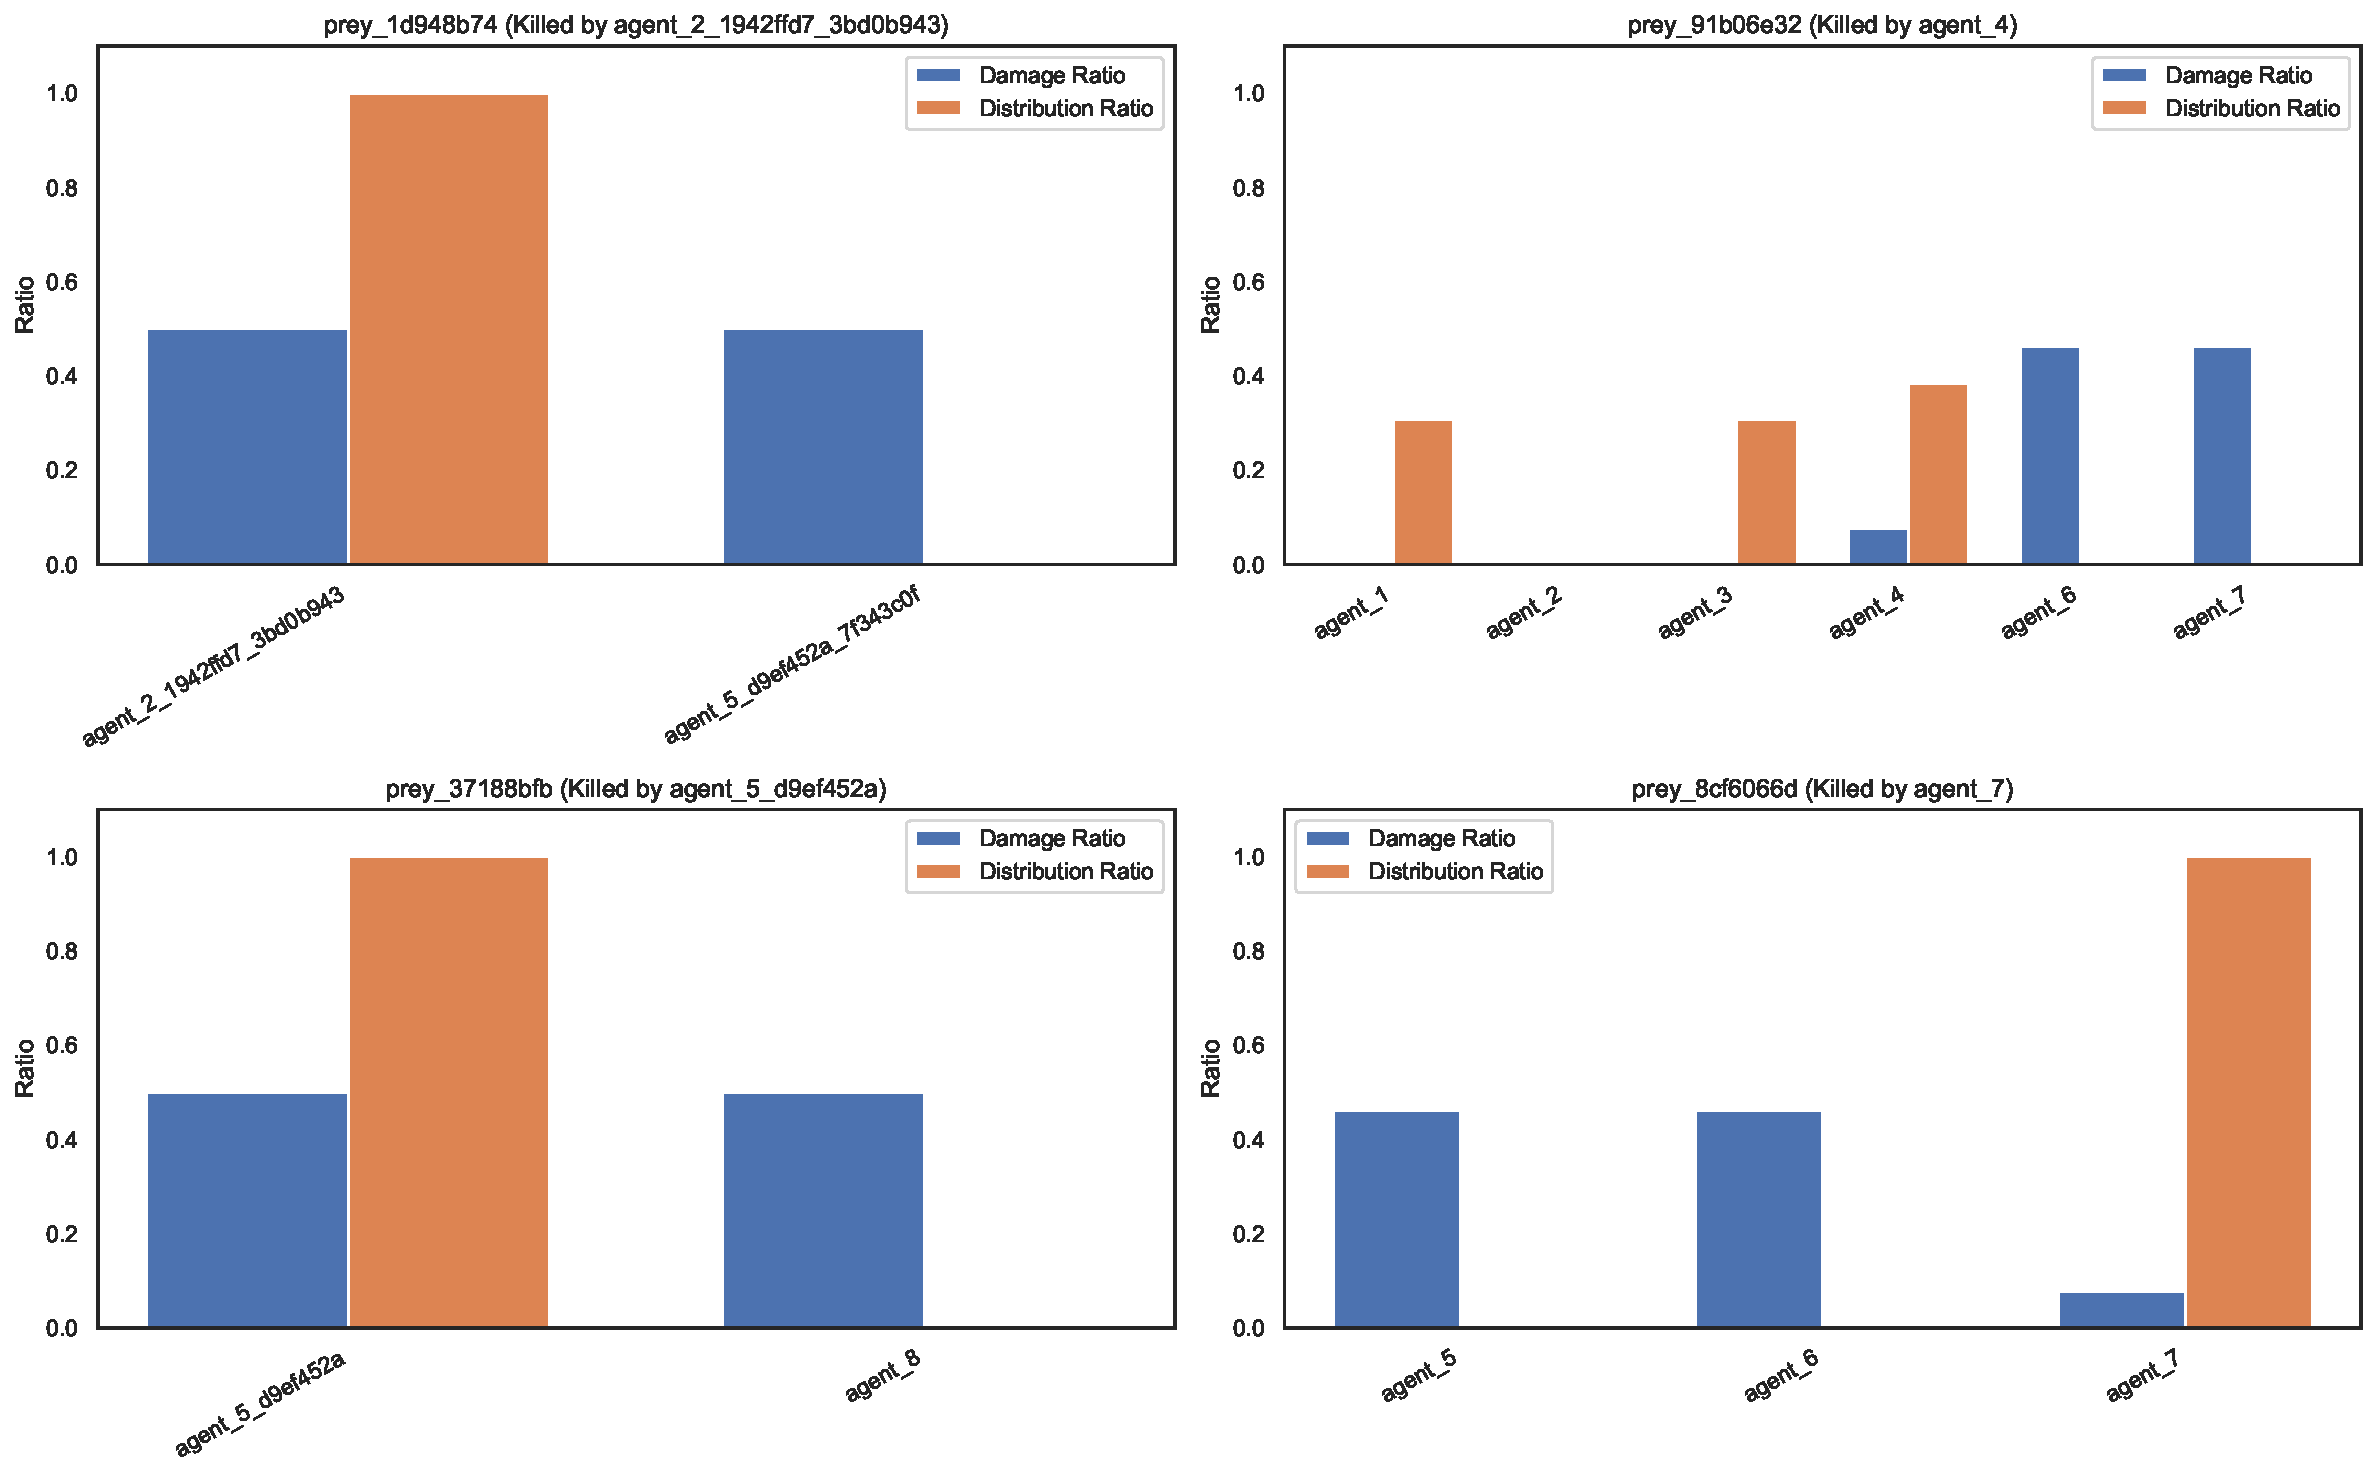
\includegraphics[width=\linewidth]{appendix_figures/prey_hunt_distribution_main.pdf}
    \caption{Selected prey hunt and HP distribution for major baseline}
    \label{fig: hunt distribution main}

\end{figure}

\subsection{Validation of Agent Behavior-Morality Alignment}

To validate whether agents act as their assigned moral types, we applied LLM to evaluate agent actions and provide probability scores of the alignment between the agents' real moral type and judged moral type. 
The confusion matrices presented in Figure~\ref{fig:confusion_matrix} illustrate the classification performance of moral types across various simulation settings. Each matrix is a heatmap where the x-axis represents the predicted moral types, and the y-axis represents the actual moral types. Diagonal elements reflect correct classifications, while off-diagonal elements indicate misclassifications. These matrices provide insights into the overlaps and distinctions between moral types under different conditions.

Overall, the results indicate that the agent performs as prompted. The confusion matrices in Figure~\ref{fig:confusion_matrix} (e), Figure~\ref{fig:confusion_matrix} (b), and (c) demonstrate high classification accuracy, with most predictions concentrated along the diagonal, in the major baseline scenario.
However, in Figure~\ref{fig:confusion_matrix} (a) and (d), there are some misclassifications, indicating overlaps between certain moral types, especially reciprocal moral and kin-focused moral agents.

\begin{figure}[H]
    \centering
    \begin{subfigure}[t]{0.32\textwidth}
        \centering
        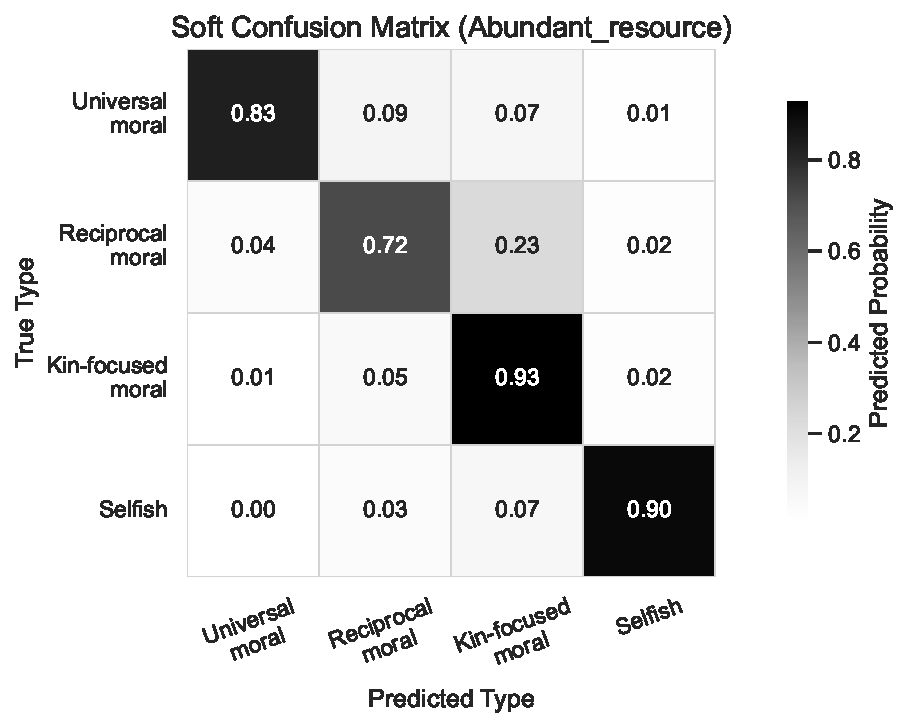
\includegraphics[width=\linewidth]{appendix_figures/matrix/Abundant_resource_soft_confusion_matrix.pdf}
        \caption{Case: abundant resource}
    \end{subfigure}
    \hfill
    \begin{subfigure}[t]{0.32\textwidth}
        \centering
        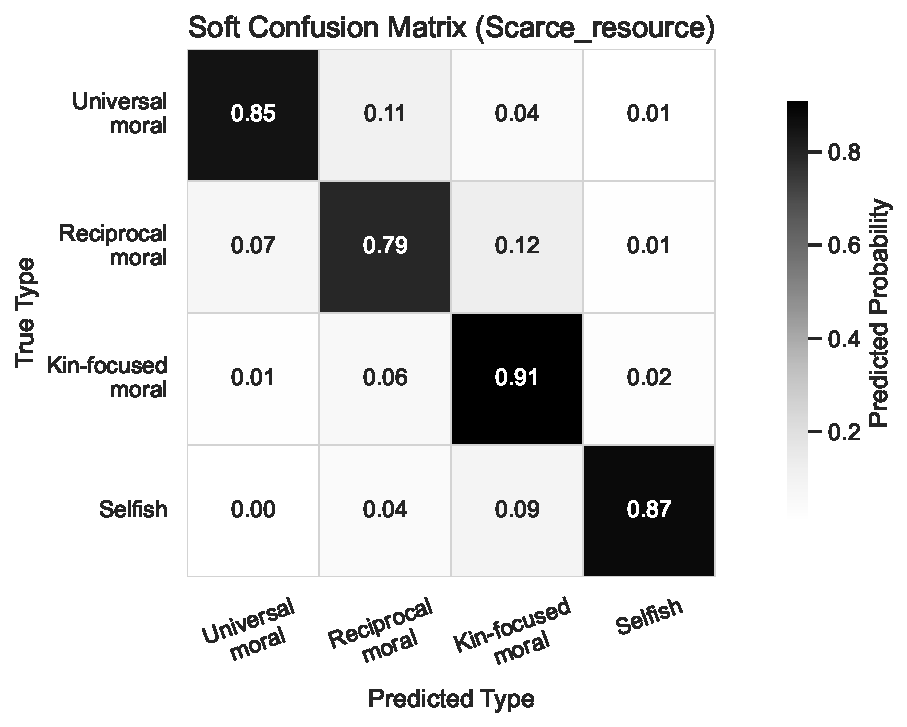
\includegraphics[width=\linewidth]{appendix_figures/matrix/Scarce_resource_soft_confusion_matrix.pdf}
        \caption{Case: scarce resource}
    \end{subfigure}
    \hfill
    \begin{subfigure}[t]{0.32\textwidth}
        \centering
        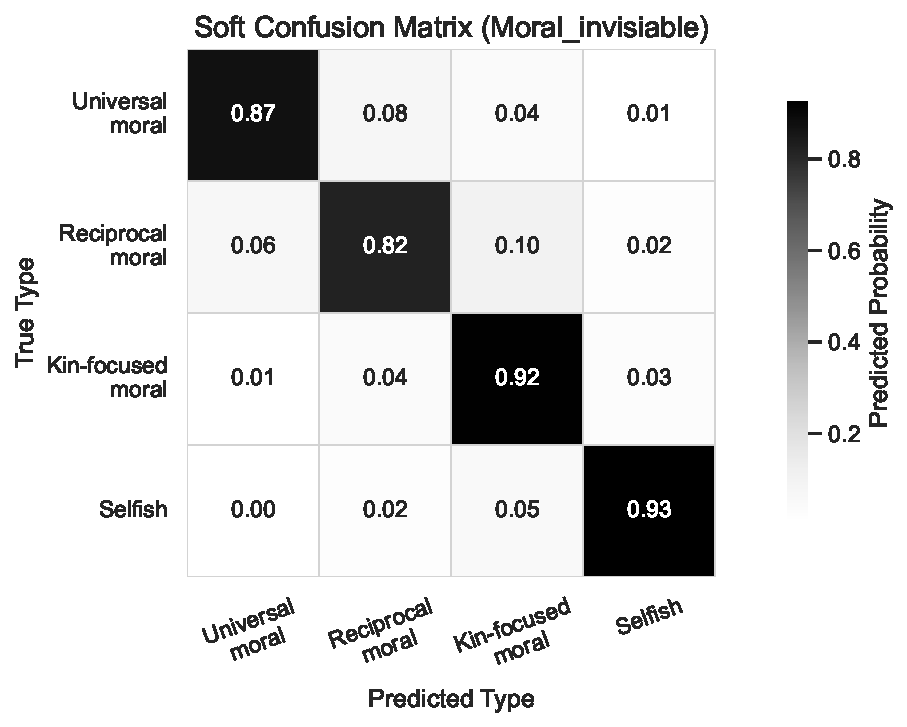
\includegraphics[width=\linewidth]{appendix_figures/matrix/Moral_invisiable_soft_confusion_matrix.pdf}
        \caption{Case: moral invisible}
    \end{subfigure}
    \hfill
    \begin{subfigure}[t]{0.32\textwidth}
        \centering
        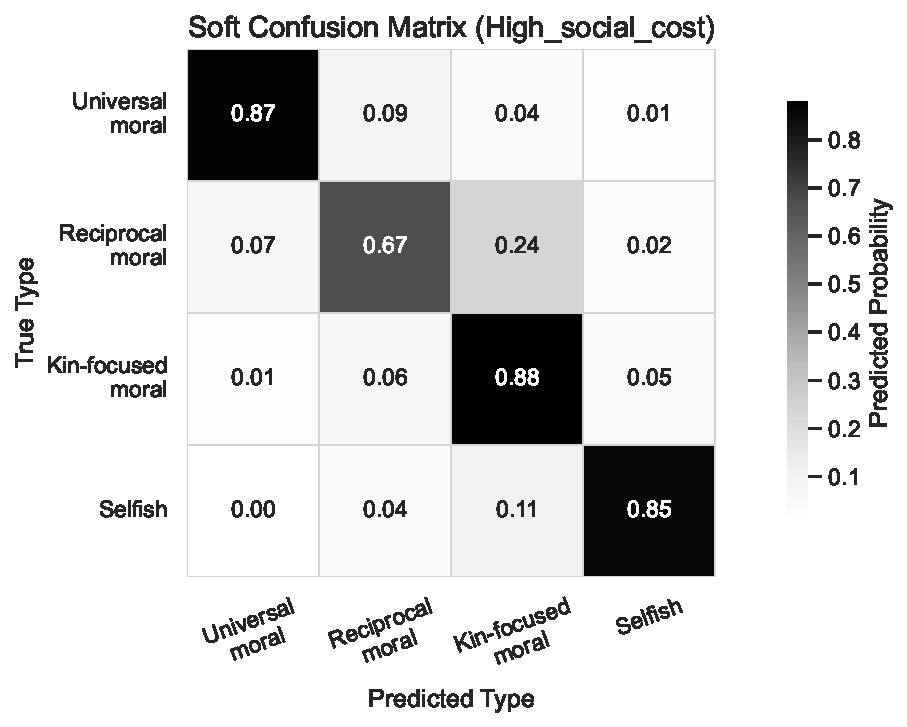
\includegraphics[width=\linewidth]{appendix_figures/matrix/High_social_cost_soft_confusion_matrix.pdf}
        \caption{Case: high social cost}
    \end{subfigure}
    \begin{subfigure}[t]{0.32\textwidth}
        \centering
        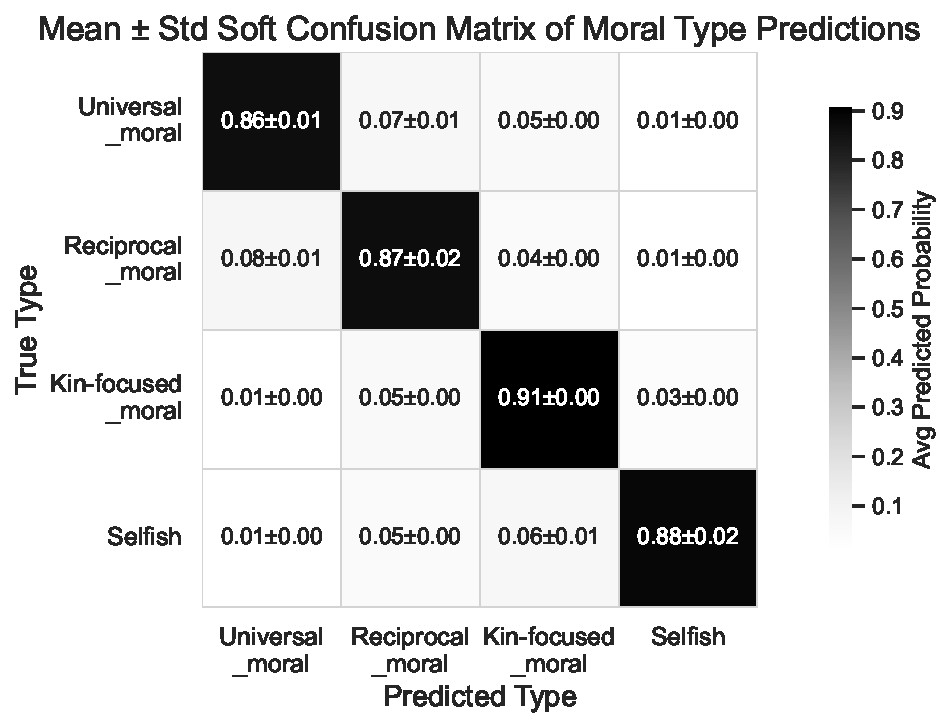
\includegraphics[width=\linewidth]{appendix_figures/matrix/Main_confusion_matrix.pdf}
        \caption{Confusion matrix for moral type test (Case: major baseline)}
    \end{subfigure}
    \caption{Confusion Matrices for moral type test in different simulation settings}
    \label{fig:confusion_matrix}
\end{figure}


\subsection{Additional Mini-Games}

\subsubsection{Game 1: Invitation Preference}


\begin{figure*}[ht]
  \centering
  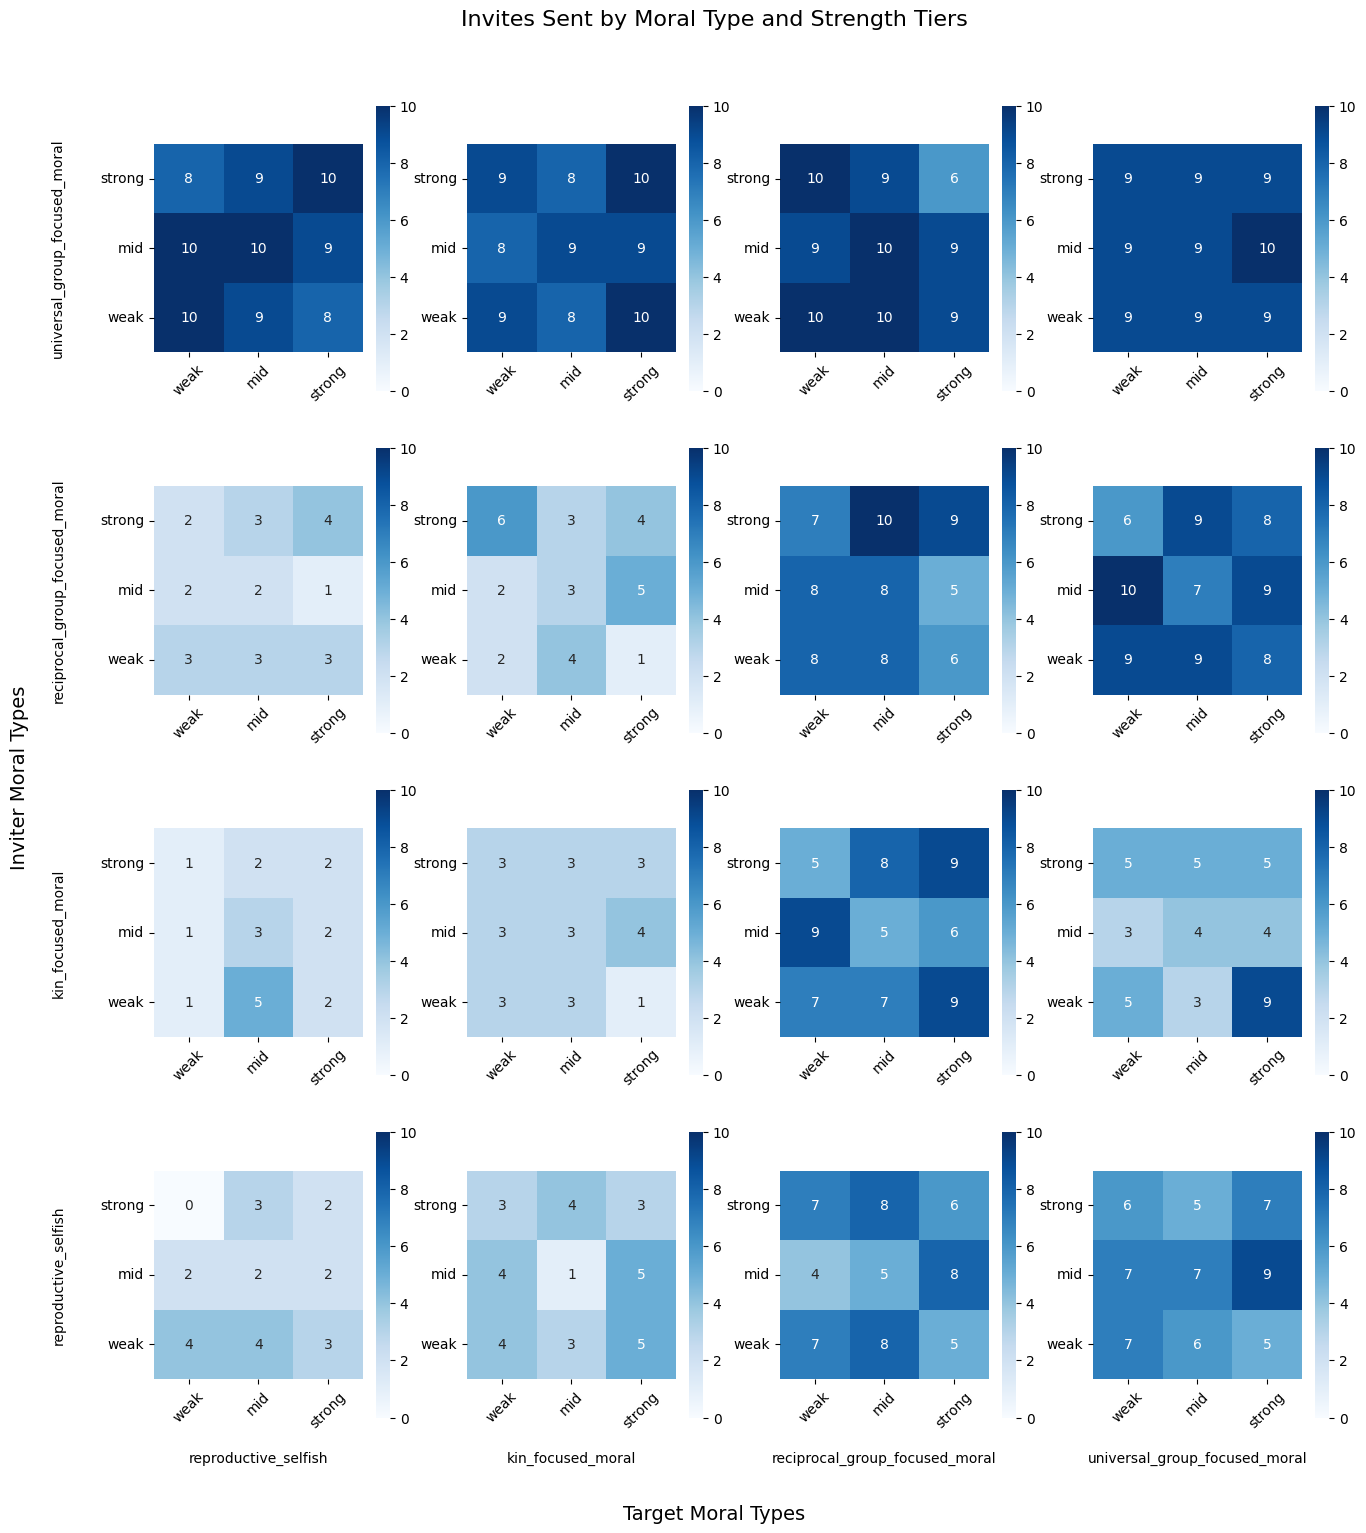
\includegraphics[width=\textwidth]{appendix_figures/mini_game_1.png}
  \caption{Invitation Distribution Among Agents. The columns represent the attributes of sender agents, while the rows correspond to those of receiver agents. Each cell in the matrix indicates the number of times (out of 10) that a sender agent issued an invitation to a receiver agent. Universal agents exhibit a consistent pattern of inviting across all types, reflecting their inclusive and group-oriented nature. In contrast, the other 3 agent types all extend significantly fewer invitations to selfish and kin-focused counterparts, showing the attraction in team forming of reciprocal and universal agents.}
  \label{fig:your-label}
\end{figure*}


What kind of partner does an agent like to invite as his/her partner? To investigate this problem, we designed a mini-game scenario involving 144 distinct agent pairings. Each agent is characterized by a combination of moral type—universal, reciprocal, kin-focused, or reproductive selfish—and physical ability—strong, mid, or weak—yielding 12 unique agent profiles. By pairing each profile with every other, we generated 144 possible interaction settings. Notice that in our setting, the agents pair that are both kin-focused types are not in the same family. 

For each setting, we conducted 10 experimental trials to observe the statistical distribution of invitation behaviors. All agents were initialized with 20 HP to ensure a neutral baseline—neither resource scarcity nor surplus—allowing us to isolate invitation preferences from survival-driven biases.

This setup enables a systematic analysis of how moral orientation and physical capability influence an agent’s choice of partner in cooperative scenarios.



\paragraph{Results}
Universal agents consistently extended invitations to all agents across different moral types and physical abilities, in line with their character, to maximize group gain and care for others. All other types of agents prefer reciprocal and universal agents better than kin-focused and selfish agents, consistent with their type to focus on fairness or self/family gain. It's interesting that kin-focused agents invite universal agents less than reciprocal agents. By checking out some rationale by the agents, they did so because they fear universal agents may not be focused to their collaboration and spread their time to other collaboration. Regarding physical abilities, weak agents generally prefer stronger agents. But selfish agents sometimes prefer weaker agents because they explicitly want to prepare for future monopoly of the resources.


% Summary of Key Patterns:
% * Moral Type Dominates Invitation Decisions: The moral type of an agent plays a more significant role than physical ability in determining invitations, with universal agents reaching out across all moral types, while reciprocal and selfish agents tend to focus more on their moral peers.
% * Physical Ability and Strategy: Stronger agents tend to invite those of similar or greater strength, though weak agents prefer stronger partners, possibly indicating strategic decision-making.
% * Moral Cooperation vs. Self-Interest: Universal and reciprocal agents tend to favor broader cooperation and fairness, while kin-focused and selfish agents are more inclined toward specific, high-value partnerships, reflecting their respective strategies of long-term collaboration versus immediate reproductive success.

% ⠀

% \subsection{
%     interesting findings:
%     1. Kin-focused agents consistently send fewer invitations to universal agents compared with reciprocal agents. This is because universal agents are sometimes perceived by kin-focused agents as ``too broad in focus" to be effective hunting partners, and may not allocate as many resources as reciprocal agents, who share a similar value of mutual aid, tightly-knit bonds, and direct alliances. This demonstrates the kin-focused agents' preference for partners with a similar focus on fairness and group success, which deviates from the universal agents' broad, inclusive approach. 
%     2. Selfish agents send fewer invitations overall compared with others, and sometimes invite weaker partners more often than stronger ones. This is because they prioritize individual gains and want to avoid resource sharing, which could reduce their own benefits. Inviting others also introduces the risk of dependence on others, as they would need to rely on partners for success, something selfish agents aim to avoid. Additionally, selfish agents seek to hoard resources to maximize their own survival, preferring to keep everything for themselves rather than splitting resources with others. These behaviors reflect an evolutionary strategy focused on self-preservation and minimizing cooperation to maintain control over resources.
% }

\subsubsection{Game 2: HP Sharing}


To understand how moral dispositions shape resource sharing within families, we studied intergenerational transfers between parents and children. Our experiment involved parent-child dyads from two distinct life stages: young parents with infants and elderly parents with adult children. We modeled four moral dispositions—reproductive selfishness, universal group-focus, reciprocal group-focus, and kin-focus—creating eight unique scenarios. For each, we generated a heatmap to visualize parental transfer behavior. In these maps, the x- and y-axes represent the parents' and child's health (HP), respectively, while the color indicates the amount of resources transferred. The results reveal that provisioning strategies are systematically driven by moral type, showing clear thresholds for initiating aid, different sensitivities to self versus offspring health, and complex interactions between moral orientation and age.

\begin{figure*}
    \centering
    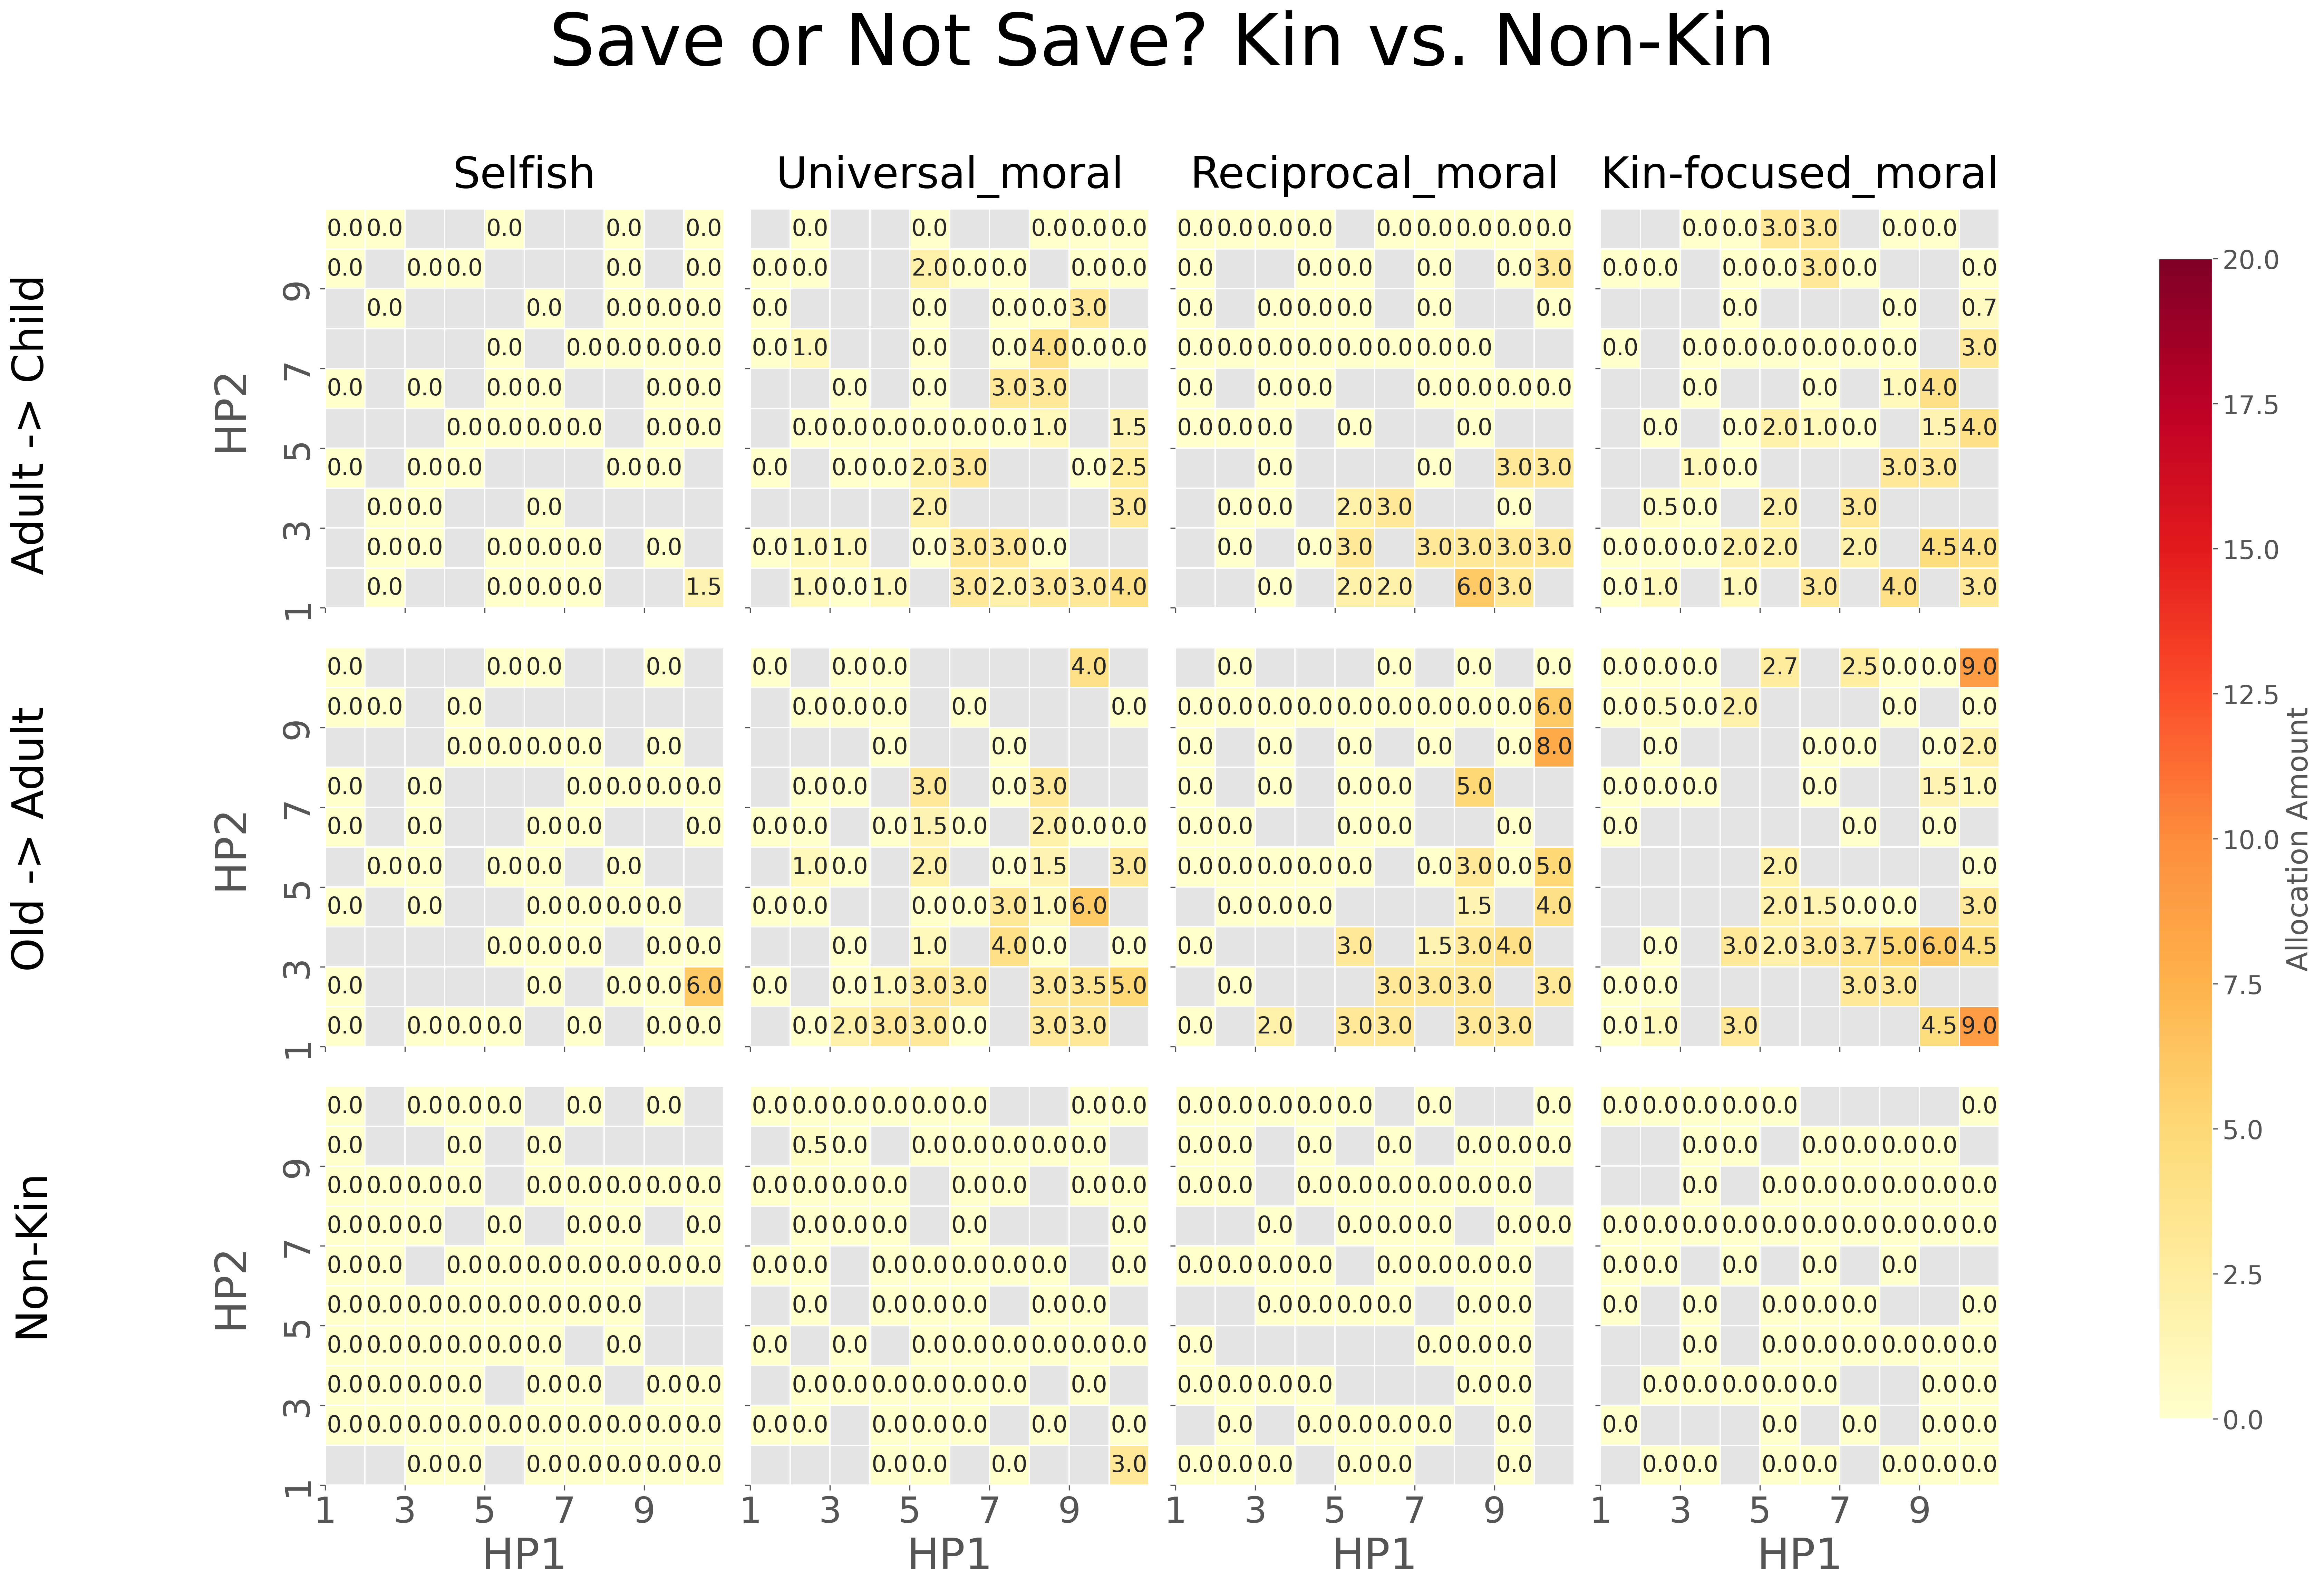
\includegraphics[width=0.8\linewidth]{figures/allocation_heatmaps_kin.png}
    \caption{Comparison of HP allocation to kin versus non-kin targets when an agent decides whether to distribute resources.}
    \label{fig:allocate_kin}
\end{figure*}
As shown in Figure~\ref{fig:allocate_kin}, we conducted additional experiments to complement the findings, specifically examining HP allocation under low HP conditions across different sender moral types. The results demonstrate that kin targets are significantly more likely to receive life-saving HP allocations than non-kin targets, even when the sender has universal moral principles.


\begin{figure*}
    \centering
    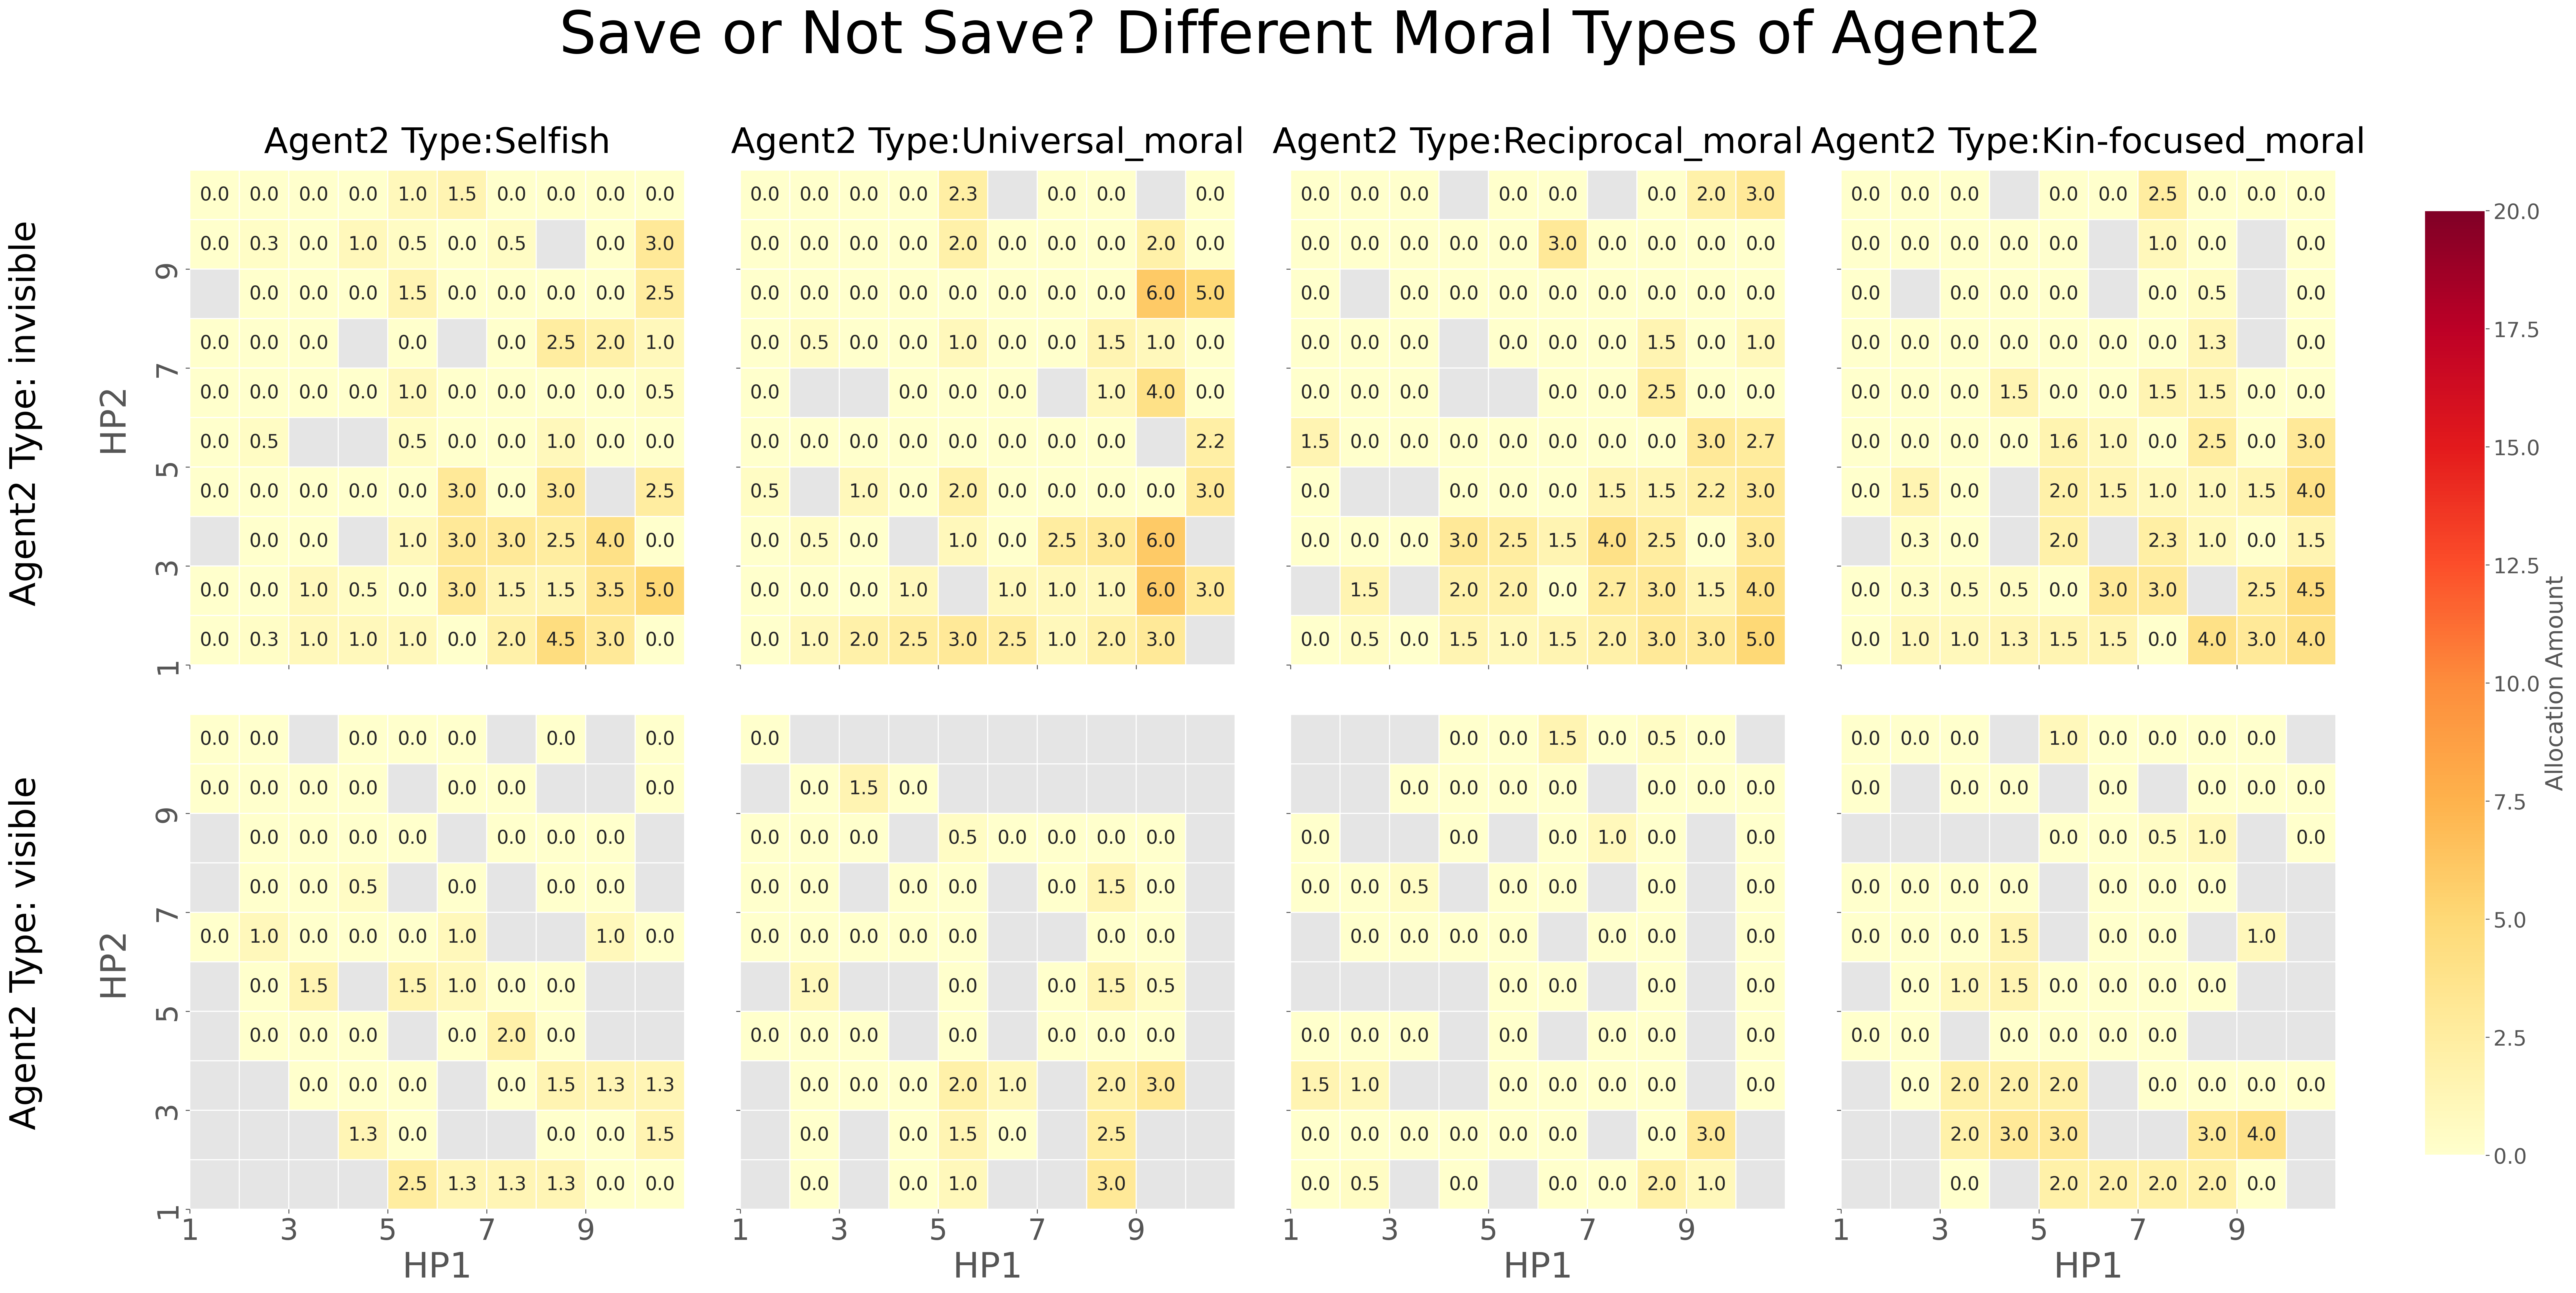
\includegraphics[width=0.8\linewidth]{figures/allocation_heatmaps_moraltype2.png}
    \caption{Comparison of HP allocation to different target moral types when an agent decides whether to distribute resources.}
    \label{fig:allocate_moraltype2}
\end{figure*}
As illustrated in Figure~\ref{fig:allocate_moraltype2}, we also investigated whether the moral type of target agents influences senders' decisions regarding life-saving HP allocation. The results indicate no significant differences in allocation behavior across target moral types.


% \begin{figure*}
%     \centering
%     
\includegraphics[width=0.8\linewidth]{figures/allocation_heatmaps_highlowhp.png}
%     \caption{Caption}
%     \label{fig:allocate_highlowhp}
% \end{figure*}